\documentclass[12pt]{article} % JASA and arxiv

\usepackage{etoolbox}

% Set this toggle true to compile a version for the arxiv, and
% false to compile for the currently configured conference.
%
% Note that if arxiv is true, then the supplement and main file
% are combined into a single pdf, but if it is false, then
% the supplement and main file are compiled separately.
\newbool{arxiv}

%\booltrue{arxiv}
\boolfalse{arxiv}


% Set whether the authors are anonymized
\newbool{blind}

\ifbool{arxiv}{
    % For arxiv
    \usepackage[style=authoryear,natbib=true]{biblatex}
    \addbibresource{references.bib}
    \usepackage{hyperref}

    \addtolength{\oddsidemargin}{-.5in}%
    \addtolength{\evensidemargin}{-1in}%
    \addtolength{\textwidth}{1in}%
    \addtolength{\textheight}{1.7in}%
    \addtolength{\topmargin}{-1in}%

} {

    % For JASA
    \usepackage[style=authoryear,natbib=true,maxbibnames=10]{biblatex}
    \addbibresource{references.bib}
    \usepackage[hidelinks=True]{hyperref}

    \def\spacingset#1{\renewcommand{\baselinestretch}%
    {#1}\small\normalsize} \spacingset{1.0}

    % DON'T change margins - should be 1 inch all around.
    \addtolength{\oddsidemargin}{-.5in}%
    \addtolength{\evensidemargin}{-1in}%
    \addtolength{\textwidth}{1in}%
    \addtolength{\textheight}{1.7in}%
    \addtolength{\topmargin}{-1in}%

    %\booltrue{blind}
    \boolfalse{blind}

}





\usepackage{microtype}
\usepackage{graphicx}
\usepackage{subfigure}
\usepackage{booktabs} % for professional tables
\usepackage{xcolor}
\usepackage{xargs}[2008/03/08]

\usepackage{enumitem} % For unseparated item bullets

% Documentation
% http://ftp.math.purdue.edu/mirrors/ctan.org/macros/latex/contrib/refstyle/refstyle.pdf
\usepackage{refstyle}
\usepackage{varioref} % Use refstyle instead of varioref directly.

\usepackage{amsmath}
\usepackage{amssymb}
\usepackage{amsfonts}
\usepackage{amsthm}
\usepackage{mathrsfs} % For mathscr
\usepackage{mathtools}
\usepackage{bm} % For bold math symbols
\usepackage{thmtools} % For QED after examples
\usepackage{accents} % For fancier accents to notate limiting values

% For algorithms
\usepackage{algorithm}
% http://tug.ctan.org/macros/latex/contrib/algorithmicx/algorithmicx.pdf
\usepackage{algpseudocode}
\usepackage{pdfpages}


\usepackage{setspace}
\renewcommand*{\bibfont}{\singlespacing} % single spaced bib

% Required for JASA to have separate main a supplement files with cross referencing
 \usepackage{xr}



% \setlength fixes todonotes; see section 1.6.5 of todonotes manual
% http://tug.ctan.org/macros/latex/contrib/todonotes/todonotes.pdf
%\setlength{\marginparwidth}{2cm}
% \usepackage[textsize=tiny]{todonotes}
%\usepackage[disable]{todonotes}


% Comment out to hide labels
%\usepackage[final]{showlabels}
%\renewcommand{\showlabelfont}{\small}
% \usepackage{rotating}
% \renewcommand{\showlabelsetlabel}[1]
% {\begin{turn}{90}\showlabelfont #1\end{turn}}


%%%%%%%%%%%%%%%%%%%%%%%%%
%       SHOW LABELS     %
%%%%%%%%%%%%%%%%%%%%%%%%%

\newbool{showlabels}

%\booltrue{showlabels}
\boolfalse{showlabels}


\ifbool{showlabels} {
    \usepackage[inline]{showlabels}
    \renewcommand{\showlabelsetlabel}[1] {
        { \tiny \showlabelfont #1 }
    }    
}

\ifbool{arxiv}{

    \newbool{largespacing}

    % Set true for editing
    %\toggletrue{largespacing}
    \boolfalse{largespacing}
    \ifbool{largespacing}{%
        \doublespacing
        \usepackage{showkeys}
    }
    % What about this one?
    %https://ctan.org/pkg/apxproof
}


%%%%%%%%%%%%%%%%%%%%%%%%%%%%%%%%%%%%%%%%%%
%%%%%%%%%%%%%%%%%%%%%%%%%%%%%%%%%%%%%%%%%%
%%%%%%%%%%%%%%%%%%%%%%%%%%%%%%%%%%%%%%%%%%


% This picks up the knitr boilerplate, allowing us to \input partial knitr
% documents.
\input{_knitr_header.tex}

% Paper-specific math macros.
\def\undernote#1#2{\underbrace{#1}_{\mathclap{\substack{#2}}}}
\def\overnote#1#2{\overbrace{#1}^{\mathclap{\substack{#2}}}}
\def\intertxt#1{\quad\textrm{#1}\quad}

% Operators
\def\ind#1{\mathbb{I}\left(#1\right)}
\def\abs#1{\left\vert #1\right\vert }
\def\norm#1{\left\Vert #1\right\Vert }
\def\evalat#1#2{\left.#1\right|_{#2}}
\def\fracat#1#2#3{\left.\frac{#1}{#2}\right\vert_{#3}}
\def\iid{\overset{iid}{\sim}}
\def\indep{\overset{indep}{\sim}}
\DeclareMathOperator*{\argmax}{\mathrm{argmax}}
\DeclareMathOperator*{\argsup}{\mathrm{argsup}}
\def\trans{\intercal}   % transpose
\def\diag#1{\mathrm{diag}\left(#1\right)}
\def\trace#1{\mathrm{tr}\left(#1\right)}

% Modes of convergence
\def\plim{\xrightarrow[N\rightarrow\infty]{prob}\,}
\def\dlim{\xrightarrow[N\rightarrow\infty]{dist}\,}


% Expectation and centering
\def\expect#1#2{\underset{#1}{\mathbb{E}}\left[#2\right]}
\def\cov#1#2{\underset{#1}{\mathrm{Cov}}\left(#2\right)}
\def\var#1#2{\underset{#1}{\mathrm{Var}}\left(#2\right)}
\def\covhat#1#2{\underset{#1}{\widehat{\mathrm{Cov}}}\left(#2\right)}

\def\p{\mathbb{P}}
\def\post{\p(\theta | \xvec)}
\def\postw{\p(\theta | \xvec; \wvec)}
\def\prob#1#2{\underset{#1}{\p}\left(#2\right)}

% MrP notation
\def\target{T}
\def\survey{S}

% Data distribution
\def\fdist{\mathbb{F}}
%\def\xfdist{\xvec\iid\fdist}
\def\xfdist{\fdist(\xvec)}

% Prior
\def\prior{\pi}
\def\logprior{\log\pi}
\def\logpriorgrad#1{\left(\logprior\right)_{(#1)}}

% Variants of the normal distribution
\def\normdist{\mathcal{N}}
\def\normhatarg#1{\hat{\mathcal{G}}(#1)}
\def\normresid#1#2{\mathcal{G}_{#1}^{#2}}
\def\normhat{\normhatarg{\tau}}
\def\normalizer{\hat{Z}}  % Normalizing constant for the Normal approximation
\def\normfourth{\hat{\mathcal{M}}} % Array of normal fourth moments


% Summation and product shortcuts
\def\sumn{\sum_{n=1}^N}
\def\summ{\sum_{m=1}^N}
\def\meann{\frac{1}{N}\sum_{n=1}^N}
\def\indexset{\mathcal{S}}
\def\means{\frac{1}{|\indexset|}\sum_{s \in \indexset}}

% Observations and functions of interest
\def\g{g}   % Function of interest
\def\y{y}   % Response variable
\def\x{x}   % A single IID datapoint
\def\xn{x_{*}}  % A generic datapoint for integrating out
\def\xvec{{\mathcal{X}}}    % All the data
\def\z{z}   % MrP regressor
\def\zn{z_{*}}   % MrP regressor
\def\yn{\y_{*}}   % Response variable
\def\t{t}   % Path variable for von Mises expansion
\def\onevec{1_N}    % Bootstrap weights all ones

% Domains and dimension
\def\thetadom{\Omega_\theta}
\def\rdom#1{\mathbb{R}^{#1}}
\def\thetaball#1{B_{#1}}
\def\ydim{D_{y}}   % Dim of sufficient statistics
\def\gdim{D_g}  % Dimension of g(\theta)
\def\thetadim{D_\theta}  % This is not used everywhere, TODO(use it everywhere)
\def\ng{\mathscr{N}_g}  % Observation indices in group g


\def\deltaulln{\delta_{LLN}}

% Information matrix stuff
\def\info{\mathcal{I}}
\def\infoev{\lambda_\mathcal{I}}
\def\infoevhat{\hat{\lambda}_\mathcal{I}}
\def\infohat{\hat{\mathcal{I}}}

% Optima and related features of the log likelihood
\def\scorecov{\Sigma}
\def\scorecovhat{\hat\Sigma}
% \def\thetatrue{\accentset{\infty}{\theta}}
% \def\gammatrue{\accentset{\infty}{\gamma}}
\def\thetatrue{\theta_{\infty}}
\def\gammatrue{\gamma_{\infty}}
\def\thetahat{\hat\theta}
\def\gammahat{\hat\gamma}
\def\thetatil{\tilde{\theta}}   % Taylor series intermediate value

\def\gammabar{\overline{\gamma}}


\def\ghat{\hat{\g}} % G centered at MAP

% BCLT residuals
\def\resid#1{\mathscr{R}^{#1}}

% Taylor series residual
\def\tresid#1#2{\mathscr{T}_{(#1)}\left(#2\right)}

% The regular event
\def\regevent{\mathfrak{R}}

% Covariances of g(\theta)
\def\gmeantrue{\mu^g}   % The true average posterior expectation
\def\gcovtrue{V^g}
\def\gcovmaphat{\hat{V}^{\mathrm{Sand}}}
\def\gcovhat{\hat{V}^{g}}
\def\gcovij{V^{\mathrm{IJ}}}
\def\gcovijhat{\hat{V}^{\mathrm{IJ}}}
\def\gcovboothat{\hat{V}^{\mathrm{Boot}}}
\def\gcovboot{V^{\mathrm{Boot}}}
\def\gcovbayeshat{\hat{V}^{\mathrm{Bayes}}}
\def\gcovbayes{V^{\mathrm{Bayes}}}

% Influence function)
\def\infl{\psi}
%\def\infltil{\accentset{\infty}{\psi}}
\def\infltil{\psi^{0}}
\def\inflalt#1{\psi^{#1}}
\def\inflhat{\hat{\psi}}

% Data weights
\def\w{w}
\def\wvec{\mathcal{W}}



% Taylor expansion and gradient notation
\def\ggrad#1{g_{(#1)}}
\def\psigrad#1{\psi_{(#1)}}
\def\ellgrad#1{\ell_{(#1)}}
\def\phigrad#1{\phi_{(#1)}}
\def\psigrad#1{\psi_{(#1)}}
\def\tgrad{\mathfrak{d}T}


% Order notation
\def\ord#1{O\left(#1\right)}
\def\ordlog#1{\tilde{O}\left(#1\right)}
\def\ordlogp#1{\tilde{O}_p\left(#1\right)}
\def\ordp#1{O_p\left(#1\right)}
\def\littleop#1{o_p\left(#1\right)}

% Log likelihood
\def\lik{\mathscr{L}}
\def\likf{\mathscr{L}_{\fdist}}
\def\likhat{\hat{\mathscr{L}}}
\def\likk#1{\mathscr{L}_{(#1)}}
\def\likhatk#1{\hat{\mathscr{L}}_{(#1)}}

% Higher order notation
% Overbar is posterior centering, underbar is frequentist centering
\def\gbar{\bar{\g}}

% Note that differentiation does not preserve posterior unbiasedness
\def\gbargrad#1{\bar{\g}_{(#1)}}
\def\gbargrad#1{\g_{(#1)}}

% Differentiation does not preserve centering at $\thetahat$
\def\ghatgrad#1{\hat{\g}_{(#1)}}
\def\ghatgrad#1{\g_{(#1)}}

\def\ellbar{\bar{\ell}}
\def\ellunderbar{\underline{\ell}}
\def\ellbarbar{\underline{\ellbar}}
\def\ellbargrad#1{\bar{\ell}_{(#1)}}
\def\ellunderbargrad#1{\ellunderbar_{(#1)}}
% Note that differentiation does not preserve posterior unbiasedness
%\def\ellbarbargrad#1{\ellbarbar_{(#1)}}
\def\ellbarbargrad#1{\ellunderbargrad{#1}}
\def\ellhatunderbar{\hat{\underline{\ell}}} % X-demeaned, centered at \thetahat
\def\ellhatunderbargrad#1{\ellhatunderbar_{(#1)}}

\def\phibar{\underline{\phi}}


% Experiments and MCMC notation
\def\seboot{\Xi^{\textrm{boot}}}
\def\seijfreq{\Xi^{\textrm{IJ:freq}}}
\def\seijmcmc{\Xi^{\textrm{IJ:mcmc}}}
\def\seij{\Xi^{\textrm{IJ}}}
\def\sebayes{\Xi^{\textrm{bayes}}}
\def\zdiff{Z}
\def\normdiffij{\Delta^{\mathrm{IJ}}}
\def\normdiffbayes{\Delta^{\mathrm{Bayes}}}


% Shortcuts for repeatedly used assumptions.
\newcommand{\seeproof}[1]{(Proof \proofpageref[vref]{#1}.)}


% https://ctan.math.illinois.edu/macros/latex/contrib/thmtools/doc/thmtools-manual.pdf
\declaretheoremstyle[
  qed=$\blacktriangleleft$,
  spaceabove=-\abovedisplayskip,
]{mythmstyle}
\declaretheorem[style=mythmstyle,name=Example]{ex}
\declaretheorem[style=mythmstyle,name=Definition]{defn}
\theoremstyle{definition}


% \newenvironment{proofsketch}[1]{\textit{Proof sketch} (full proof in #1):}{\hfill$\square$}
\newenvironment{proofsketch}[1]
    {\noindent\textit{Proof sketch (full proof in #1): }}
    {\hfill$\square$\break}


%%%%%%%%%%%%%%%%%%%%
% amsthm commands

\theoremstyle{plain}
\newtheorem{lem}{Lemma}
\newtheorem{thm}{Theorem}
\newtheorem{prop}{Proposition}
\newtheorem{cond}{Condition}
\newtheorem{assu}{Assumption}
\newtheorem{cor}{Corollary}
\newtheorem{conj}{Conjecture}


% \newtheorem{defn}{Definition}
% \newtheorem{ex}{Example}

%%%%%%%%%%%%%%%%%%%%
% refstyle commands

\newref{event}{
    name=Event~, %
    names=Events~, %
    Name=Event~,
    Names=Events~
    }

\newref{item}{
    name=Item~, %
    names=Items~, %
    Name=Item~
    Names=Items~
    }

\newref{fig}{
    name=Figure~, %
    Name=Figure~
    }

\newref{tab}{
    name=Table~, %
    Name=Table~
    }

\newref{sec}{
    name=Section~, %
    Name=Section~
    }

\newref{app}{
    name=Appendix~, %
    Name=Appendix~
    }

\newref{eq}{
    name=Eq.~, %
    Name=Eq.~,
    names=Eqs.~, %
    Names=Eqs.~
    }

\newref{fig}{
    name=Figure~, %
    Name=Figure~
    }

\newref{def}{
    name=Definition~, %
    Name=Definition~
    }

\newref{assu}{
    name=Assumption~, %
    Name=Assumption~,
    names=Assumptions~, %
    Names=Assumptions~,
    }

\newref{cond}{
    name=Condition~, %
    Name=Condition~,
    names=Conditions~, %
    Names=Conditions~
    }

\newref{prop}{
    name=Proposition~, %
    Name=Proposition~,
    names=Propositions~, %
    Names=Propositions~
    }

\newref{lem}{
    name=Lemma~, %
    Name=Lemma~,
    names=Lemmas~, %
    Names=Lemmas~
    }

\newref{ex}{
    name=Example~, %
    Name=Example~}

\newref{cor}{
    name=Corollary~, %
    Name=Corollary~
    }

\newref{thm}{
    name=Theorem~, %
    Name=Theorem~,
    names=Theorems~, %
    Names=Theorems~
    }

\newref{proof}{
    name=Proof~, %
    Name=Proof~
    }

\newref{conj}{
    name=Conjecture~, %
    Name=Conjecture~
    }

\newref{algr}{
    name=Algorithm~, %
    Name=Algorithm~,
    names=Algorithms~, %
    Names=Algorithms~,
    }


%% refstyle examples:
% \Secref[vref]{introduction} contains \secref{introduction}.
% \Secref[vref]{ack} does not contain \secref{introduction}.
%
% \begin{align}
%     x=y \eqlabel{myeq}
% \end{align}
%


%%%%%%%%%%%%%%%%%%%%%%%%%%%%%%%%%%%%%%
%%%%%%%%%%%%%%%%%%%%%%%%%%%%%%%%%%%%%%
% Do not edit the TeX file your work
% will be overwritten.  Edit the RnW
% file instead.
%%%%%%%%%%%%%%%%%%%%%%%%%%%%%%%%%%%%%%
%%%%%%%%%%%%%%%%%%%%%%%%%%%%%%%%%%%%%%






\begin{knitrout}
\definecolor{shadecolor}{rgb}{0.969, 0.969, 0.969}\color{fgcolor}\begin{kframe}


{\ttfamily\noindent\bfseries\color{errorcolor}{\#\# Error in readChar(con, 5L, useBytes = TRUE): cannot open the connection}}

{\ttfamily\noindent\bfseries\color{errorcolor}{\#\# Error in readChar(con, 5L, useBytes = TRUE): cannot open the connection}}

{\ttfamily\noindent\bfseries\color{errorcolor}{\#\# Error in readChar(con, 5L, useBytes = TRUE): cannot open the connection}}\end{kframe}
\end{knitrout}

\begin{kframe}


{\ttfamily\noindent\bfseries\color{errorcolor}{\#\# Error in eval(ei, envir): object 'arm\_env' not found}}

{\ttfamily\noindent\bfseries\color{errorcolor}{\#\# Error in eval(ei, envir): object 'simple\_sim\_env' not found}}

{\ttfamily\noindent\bfseries\color{errorcolor}{\#\# Error in eval(ei, envir): object 'mrp\_env' not found}}\end{kframe}


\def\ARMTable{
\begin{table}[h]
\begin{kframe}


{\ttfamily\noindent\bfseries\color{errorcolor}{\#\# Error in eval(ei, envir): object 'arm\_env' not found}}\end{kframe}
\caption{Models from \cite{gelman:2006:arm}\tablabel{arm_models}}
\end{table}
}


\def\ARMModelList{
\begin{kframe}


{\ttfamily\noindent\bfseries\color{errorcolor}{\#\# Error in eval(ei, envir): object 'arm\_env' not found}}\end{kframe}
}


\def\ARMGraphZ{
%

\begin{knitrout}
\definecolor{shadecolor}{rgb}{0.969, 0.969, 0.969}\color{fgcolor}\begin{kframe}


{\ttfamily\noindent\bfseries\color{errorcolor}{\#\# Error in eval(ei, envir): object 'arm\_env' not found}}\end{kframe}
\end{knitrout}
}


\def\ARMGraphDiff{
%

\begin{knitrout}
\definecolor{shadecolor}{rgb}{0.969, 0.969, 0.969}\color{fgcolor}\begin{kframe}


{\ttfamily\noindent\bfseries\color{errorcolor}{\#\# Error in eval(ei, envir): object 'arm\_env' not found}}\end{kframe}
\end{knitrout}
}



\def\ARMGraphPostDiff{
%

\begin{knitrout}
\definecolor{shadecolor}{rgb}{0.969, 0.969, 0.969}\color{fgcolor}\begin{kframe}


{\ttfamily\noindent\bfseries\color{errorcolor}{\#\# Error in eval(ei, envir): object 'arm\_env' not found}}\end{kframe}
\end{knitrout}
}



%%%%%%%%%%%%%%%%%%%%%%%%%%%%%%%%%%%%%%%%%%%%%%%%%%%%%%%%%%%%%%%%%%%%%%%%%
%%%%%%%%%%%%%%%%%%%%%%%%%%%%%%%%%%%%%%%%%%%%%%%%%%%%%%%%%%%%%%%%%%%%%%%%%
%%%%%%%%%%%%%%%%%%%%%%%%%%%%%%%%%%%%%%%%%%%%%%%%%%%%%%%%%%%%%%%%%%%%%%%%%

\def\SingularResultsGraph{

\begin{knitrout}
\definecolor{shadecolor}{rgb}{0.969, 0.969, 0.969}\color{fgcolor}\begin{kframe}


{\ttfamily\noindent\bfseries\color{errorcolor}{\#\# Error in PlotVar("{}x"{}): object 'simple\_sim\_env' not found}}\end{kframe}
\end{knitrout}
%
}



%%%%%%%%%%%%%%%%%%%%%%%%%%%%%%%%%%%%%%%%%%%%%%%%%%%%%%%%%%%%
%%%%%%%%%%%%%%%%%%%%%%%%%%%%%%%%%%%%%%%%%%%%%%%%%%%%%%%%%%%%%%%%%%%%%%%%%
%%%%%%%%%%%%%%%%%%%%%%%%%%%%%%%%%%%%%%%%%%%%%%%%%%%%%%%%%%%%%%%%%%%%%%%%%
%
% <<sim_ar_vars>>=
% sim_ar <- 1.
% sim_img_over_legend <- 2
% sim_r_width <- 2.7
% @

\newcommand{\MRPGraph}{

\begin{knitrout}
\definecolor{shadecolor}{rgb}{0.969, 0.969, 0.969}\color{fgcolor}\begin{kframe}


{\ttfamily\noindent\bfseries\color{errorcolor}{\#\# Error in eval(ei, envir): object 'mrp\_env' not found}}\end{kframe}
\end{knitrout}
}


\newcommand{\MRPMAPGraph}{

\begin{knitrout}
\definecolor{shadecolor}{rgb}{0.969, 0.969, 0.969}\color{fgcolor}\begin{kframe}


{\ttfamily\noindent\bfseries\color{errorcolor}{\#\# Error in eval(ei, envir): object 'mrp\_env' not found}}\end{kframe}
\end{knitrout}
}




\newcommand{\MRPLMERGraph}{

\begin{knitrout}
\definecolor{shadecolor}{rgb}{0.969, 0.969, 0.969}\color{fgcolor}\begin{kframe}


{\ttfamily\noindent\bfseries\color{errorcolor}{\#\# Error in eval(ei, envir): object 'mrp\_env' not found}}\end{kframe}
\end{knitrout}
}


\newcommand{\MRPLMERSdGraph}{

\begin{knitrout}
\definecolor{shadecolor}{rgb}{0.969, 0.969, 0.969}\color{fgcolor}\begin{kframe}


{\ttfamily\noindent\bfseries\color{errorcolor}{\#\# Error in eval(ei, envir): object 'mrp\_env' not found}}\end{kframe}
\end{knitrout}
}



% \usepackage{lineno}
% \linenumbers




\notbool{arxiv} {
    \externaldocument{supplement}
}


\author{\paperauthor}
\title{My Paper}

\begin{document}

\title{The Bayesian Infinitesimal Jackknife for Variance}

\author{
    \ifbool{blind} {
        (ANONYMIZED)
    } {
    Ryan Giordano \\ \texttt{rgiordano@berkeley.edu}
    \and
    Tamara Broderick \\ \texttt{tbroderick@mit.edu}
    }
}


\maketitle

\notbool{arxiv} {
    % JASA

    \begin{abstract}
    %
    The frequentist variability of Bayesian posterior expectations can provide
meaningful measures of uncertainty even when models are
misspecified. However, standard methods to approximate the frequentist
covariance of posterior expectations — namely, those using the MAP estimator or
the nonparametric bootstrap — can be practically inconvenient. In particular,
the MAP estimator may behave poorly in moderate dimensions, and the bootstrap
requires computing the posterior for many different bootstrap datasets.  We
develop another method, the infinitesimal jackknife (IJ), for
estimating the frequentist variability of posterior expectations.  The IJ is a
method for computing asymptotic frequentist covariances of smooth
functionals of exchangeable data using the ``influence function'' of
robust statistics.  We show that the influence function for posterior
expectations is given by a simple posterior covariance, and that the IJ
covariance estimate is easily computed from a single set of posterior
samples. Under conditions similar to those required for a Bayesian central limit
theorem, we prove that the IJ covariance estimate is
asymptotically equivalent to that given by the sandwich covariance and the
bootstrap, but avoids reliance on an accurate MAP estimate or on bootstrap
samples. We demonstrate the accuracy and computational benefits of the IJ
covariance estimates with simulated and real-world experiments.
    %
    \end{abstract}        
    
    % Only include keywords for the journal
    \noindent%
    {\it Keywords:}  Influence function, sandwich covariance,
        infinitesimal jackknife, Bernstein-von Mises theorem,
        Bayesian robustness
    \vfill    

    
    \newpage
    %\spacingset{1.9} % DON'T change the spacing!

    % It says don't change the spacing, but then the rendering
    % does not produce the maximum allowed 26 lines per page
    \spacingset{1.8} % DON'T change the spacing!
}


% What is the frequentist variance and why would you care.
% The Laplace approximation and bootstrap have shortcomings that the IJ
% does not.
\section{Introduction}\seclabel{introduction}

% We care about posterior expectations, and these expectations have a
% frequentist variance.
% Even Bayesians should care about frequentist variances as a robustness measure.
Suppose we want to use Bayesian methods to infer some parameter or quantity of
interest from exchangeable data. The Bayesian posterior is often summarized by a
point estimate and measure of subjective uncertainty, which we will respectively
take to be the posterior mean and posterior variance.  The computed posterior
mean is a function of the observed data, and so has a well-defined frequentist
variance under re-sampling of the exchangeable data.  The Bayesian posterior
variance of a quantity and the frequentist variance of its mean are conceptually
distinct: the posterior variance can be thought of as describing the
uncertainty of subjective beliefs under the assumption of correct model
specification, and the frequentist variance captures the sensitivity of the
Bayesian point estimate to re-sampling of the observed data.  In general,
both may be of interest.
Even a strict Bayesian can meaningfully interpret the
frequentist variance of the posterior mean as a \emph{sensitivity analysis},
quantifying how much the Bayesian point estimate would vary had we received
different but realistic data.  Such a sensitivity analysis is particularly
germane when the data is known to have come from a random sample from a real
population. 


% You might think the two notions are the same, but they are not when you
% have misspecification
In general, the frequentist and Bayesian variances are not only conceptually
distinct but can be numerically very different.  It is true that, with
independent and identically distributed (IID) data, some reasonable regularity
conditions, a correctly specified model, and a parameter vector of fixed
dimension, the frequentist and Bayesian variances coincide asymptotically as a
consequence of the Bernstein--von Mises theorem, a.k.a.\ the Bayesian central limit
theorem.  However, under \emph{model misspecification}, the equality between the
frequentist and Bayesian variances no longer holds in general, even
asymptotically \citep{kleijn:2012:bvm} --- and most models are misspecified.


% Standard tools are inadequate
When posterior means are estimated using Markov Chain Monte Carlo (MCMC), the
two standard tools for estimating the frequentist variability of Bayesian
posterior expectations --- the nonparametric bootstrap  (henceforth simply
``bootstrap'') and the Laplace approximation --- can be each be problematic,
though for different reasons.
%
% The bootstrap is inadequate
To compute a bootstrap estimate of
the frequentist variance of a posterior mean, one repeatedly draws ``bootstrap
datasets,'' with replacement from the original set of datapoints. For each
bootstrap dataset, one then computes the posterior mean for each set of
re-sampled data \citep{huggins:2022:bayesbag}.  Though straightforward to
implement and naively parallelizable, the bootstrap remains
computationally expensive, since a separate posterior estimate (e.g., a
run of MCMC) must be computed for each bootstrap dataset.
%
% The Laplace approximation is inadequate
Alternatively, it is straightforward to estimate frequentist variance of a
Laplace approximation to the posterior.   Specifically, one can do so by
computing the ``sandwich covariance'' estimate of the maximum \textit{a
posteriori} (MAP) estimate at which the Laplace approximation is centered
\citep{stefanski:2002:mestimation}.  This approach essentially uses the standard
consistent estimator of the limiting covariance derived by
\citet{kleijn:2012:bvm}.  However, this approach requires using a particular Laplace
approximation to the posterior rather than MCMC and, as we show below, the
Laplace approximation can be practically and conceptually problematic.  For
example, unlike true posterior draws, the Laplace approximation is not invariant
to reparameterization, and, for some parameterizations the Laplace approximation
can fail catastrophically, especially in hierarchical models.


% We solve these problems with the IJ covariance.
In the present paper, we provide an estimator of the frequentist variability of
posterior expectations that enjoys the model-agnostic properties of the
bootstrap, but can be computed from a single run of MCMC. Our
method is based on the \emph{infinitesimal jackknife} (IJ) variance estimator, a
classical frequentist variance estimator derived from the \emph{empirical
influence function} of a statistical functional.  We show that the Bayesian
empirical influence function is easily computable as a particular set of
posterior covariances, the variance of which is a consistent estimator of the
frequentist variance of a posterior expectation when a Bayesian central limit
theorem (BCLT) holds for all model parameters.

% We potentially solve other problems.
Finally, though our present concern is frequentist variance estimates, the
empirical influence function is a powerful statistical tool, with applications
in robustness, cross validation, and bias estimation. Consequently, our results
for the influence function of Bayesian posteriors and a BCLT for expectations of
data-dependent functions are of broader interest.  We leave off exploring these
topics for future work.


\section{Setup and Motivation}\seclabel{basics}

%\subsection{Formal problem statement}
% Data and likelihood notation.
Suppose we observe $N$ data points, $\xvec = (\x_1, \ldots \x_N)$.  We will
assume that the entries of $\xvec$ are independently and identically distributed
(IID) according to a distribution $\fdist$.  In a slight abuse of notation, we
will write $\xfdist$ for $\prod_{n=1}^N \fdist(\x_n)$.  Throughout, the
distribution $\fdist$ will be taken as fixed but unknown.  A Bayesian typically
models the distribution of $\xvec$ by an IID parametric model
given on some parameters $\theta \in \thetadom \subseteq \rdom{\thetadim}$:
%
$$
\p(\xvec \vert \theta) = \prod_{n=1}^N \p(\x_n \vert \theta) = 
    \exp\left(\sumn \ell(\x_n \vert \theta) \right)
\intertxt{where}
\ell(\x_n \vert \theta) := \log \p(\x_n \vert \theta).
$$
%
In the present work, we admit that the model may be misspecified, i.e., there may be no $\theta
\in \thetadom$ such that $\p(\x_n \vert \theta)$ is the same distribution as
$\fdist$.  

We will additionally posit a prior over the parameters
$\theta$, and assume this prior can be expressed as
a density $\prior(\cdot)$ with respect to the Lebesgue measure on $\rdom{\thetadim}$.  Then
we can compute the posterior expectation of a vector-valued quantity $g(\theta)
\in \rdom{\gdim}$ using Bayes' rule:
%
\begin{align}
%
\expect{\post}{\g(\theta)} =
    \frac{
    \int_{\thetadom} g(\theta)
        \exp\left(N \meann \ell(\x_n \vert \theta) \right) \prior(\theta)
                        d\theta}
         {\int_{\thetadom}
         \exp\left(N \meann \ell(\x_n \vert \theta) \right) \prior(\theta)
         d\theta}.
         \eqlabel{g_post}
%
\end{align}

The quantity $\expect{\post}{\g(\theta)}$ is a function of the data $\xvec$,
through its dependence on the random function $\theta \mapsto \meann \ell(\x_n
\vert \theta)$.  We will be primarily concerned with the problem of how to
estimate the variability of $\expect{\post}{\g(\theta)}$ under sampling from
$\xfdist$, when $N$ is large, using Markov Chain Monte Carlo (MCMC)
samples from the posterior $\post$, in the presence of possible
misspecification.
%
% Using an estimate of its variability, one can use classical frequentist tests to
% estimate how much the posterior mean might be expected to have varied were we to
% have drawn a different sample $\xvec$.
Specifically, let $\plim$ and $\dlim$ respectively denote convergence in
probability and distribution under sampling from $\xfdist$. We will
articulate conditions under which
% The mean and covariance (if they exist) of $\expect{\post}{\g(\theta)}$ under
% sampling from $\xfdist$ can be written respectively as
%
\begin{align}\eqlabel{gtrue}
%
\expect{\post}{\g(\theta)} \plim \gmeantrue < \infty
\quad\textrm{and}\quad
\sqrt{N}\left(\expect{\post}{\g(\theta)} - \gmeantrue \right)
\dlim
\normdist\left(\cdot \vert 0, \gcovtrue\right)
% \gcovtrue_{FS} := \cov{\xfdist}{\expect{\post}{\g(\theta)}}.
%
\end{align}
for some constants $\gmeantrue$ and $\gcovtrue$.  Under these conditions, our
contribution is to form a consistent estimator of $\gcovtrue$ that can be
computed from a single set of draws from $\post$, and so approximated from a
single run of MCMC.  We emphasize that our objective of establishing
\eqref{gtrue} is weaker than estimating the limiting variance of $\sqrt{N}
\expect{\post}{\g(\theta)}$, which may not even exist, but which would coincide
with $\gcovtrue$ under an additional assumption of uniform integrability (see,
e.g., Theorem 10.3.6 of \citet{dudley:2018:realanalysis}).




%%%%%%%%%%%%%%%%%%%%%%%%%%%%%%%%%%%%%
%%%%%%%%%%%%%%%%%%%%%%%%%%%%%%%%%%%%%

% Outline of the rest of the paper.




\subsection{Notation}\seclabel{notation}
We will begin by defining some notation. Given a distribution $\p(t)$ and an
integrable function $\phi(t)$, we will use the expectation operator as a formal
shorthand for the integral
%
%\begin{align*}
$\expect{\p(t)}{\phi(t)} = \int \phi(t) \p(dt)$.
%\end{align*}
%
Any quantities not explicitly part of the distribution beneath the expectation
operator should be thought of as fixed. Covariances and variances are treated
similarly, i.e.\,
%
%\begin{align*}
%
$\cov{\p(t)}{\phi(t), \psi(t)} =
    \expect{\p(t)}{\phi(t) \psi(t)^T} -
        \expect{\p(t)}{\phi(t)} \expect{\p(t)}{\psi(t)}^T$.
%
%\end{align*}
%
We will denote sample covariances over an index $n \in \{1,
\ldots, N \} = [N]$ as $\covhat{n \in [N]}{\cdot, \cdot}$.
% %
% \begin{align*}
% %
% \covhat{n \in [N]}{s_n, t_n} :={}& \frac{1}{N}
%     \sumn s_n t_n - \left( \meann s_n \right) \left( \meann t_n \right)^T.
% %
% \end{align*}

We denote partial derivatives with respect to $\theta$ with bracketed
subscripts.  For example, for a function $\psi(\theta)$ taking values in
$\rdom{D_\psi}$, let $\psigrad{k}(\theta)$ denote the array of $k$-th order
partial derivatives with respect to $\theta$, i.e.,
%
%\begin{align*}
%
$
\psigrad{k}(\theta) :=
    \fracat{\partial^k \psi(\theta)}{\partial\theta^k}{\theta}.
$
%
%\end{align*}
%
If $\psi$ depends on any variables other than $\theta$, those variables will be
taken as fixed in the partial differentiation.
%
In general, $\psigrad{k}(\theta)$ is an array with $D_\psi \thetadim^k$ entries, and we
will introduce special notation as needed when summing over the array's entries.
But we will mostly be able to avoid such special notation by interpreting the
following special cases in standard matrix notation:
%
% \begin{itemize}
% %
% \item When $D_\psi = 1$ and $k = 1$, $\psigrad{1}(\theta)$ is taken to be a
% $\thetadim$-column vector.
% %
% \item When $D_\psi > 1$ and $k = 1$, $\psigrad{1}(\theta)$ is taken to be a
% $D_\psi \times \thetadim$ matrix.
% %
% \item When $D_\psi = 1$ and $k=2$, $\psigrad{2}(\theta)$ is taken to be a $\thetadim
% \times \thetadim$ matrix.
% %
% \item When $k = 0$, $\psigrad{0}(\theta)$ is just $\psi(\theta)$.
% %
% \end{itemize}
%
when $D_\psi = 1$ and $k = 1$, $\psigrad{1}(\theta)$ is taken to be a
$\thetadim$-column vector; when $D_\psi > 1$ and $k = 1$, $\psigrad{1}(\theta)$
is taken to be a $D_\psi \times \thetadim$ matrix; when $D_\psi = 1$ and $k=2$,
$\psigrad{2}(\theta)$ is taken to be a $\thetadim \times \thetadim$ matrix; and
when $k = 0$, $\psigrad{0}(\theta)$ is just $\psi(\theta)$.


% Define likelihood and related quantities
Our proposal and existing methods for estimating $\gcovtrue$ will depend on some key
quantities to which we give symbols in \defref{loglik_def}.  In the left hand
column of \defref{loglik_def} we have finite-sample quantities, and on the right
hand side we have the corresponding population quantities. In \secref{bayes_clt}
below we will state precise conditions under which all the quantities of
\defref{loglik_def} are well-defined.  We will use $\xn$ to denote a generic
single datapoint, in contrast to specific observed datapoints, $\x_n$.
%
\begin{defn}\deflabel{loglik_def}
\setlength{\abovedisplayskip}{0pt}
\setlength{\abovedisplayshortskip}{0pt}
\begin{align*}
&\textrm{Finite-sample quantity} && \textrm{Population quantity}\\
%
\likhat(\theta) :={}&
   \frac{1}{N} \sumn \ell(\x_n \vert \theta) +
   \frac{1}{N} \logprior(\theta)
&
\quad \lik(\theta) :={}& \expect{\fdist(\xn)}{\ell(\xn \vert \theta)}
\\
\thetahat :={}& \argmax_{\theta \in \thetadom} \likhat(\theta)
&
\thetatrue :={}& \argmax_{\theta \in \thetadom} \lik(\theta)
\\
\scorecovhat :={}&
   \frac{1}{N} \sumn \ellgrad{1}(\x_n \vert \thetahat)
                     \ellgrad{1}(\x_n \vert \thetahat)^T
&
\scorecov :={}&
    \cov{\fdist(\xn)}{\ellgrad{1}(\xn \vert \thetatrue)}
\\
% \infohat :={}& -\fracat{\partial^2 \likhat(\theta)}
%                      {\partial\theta \partial\theta^T}{\thetahat}
\infohat :={}& -\likhatk{2}(\thetahat)
&
\info :={}& - \expect{\fdist(\xn)}{\ellgrad{2}(\xn \vert \thetatrue)} \qedhere
%
\end{align*}
\end{defn}
%

% We are studying fixed frequentist properties.
We will take the population quantities in the right column of
\defref{loglik_def} to be fixed (though, in general, unknown) and study the
sampling behavior of quantities in the left column. That is, we will study the
asymptotic behavior of formal Bayesian posterior quantities as a function of a
fixed data generating process, following much of the literature on the
frequentist behavior of Bayesian estimators (e.g., \citet{van:2000:asymptotic}).
% Note that the numeric vector $\thetatrue$ is
% conceptually distinct from the random variable $\theta$ of the Bayesian
% posterior, despite also existing in $\thetadom$.
%
Our notation for stochastic convergence reflects these assumptions.  In
particular, order notation $O(\cdot)$ applies as $N \rightarrow \infty$, and
probabilistic order notation $O_p(\cdot)$ denotes order in probability over
$\fdist(\xn)$.  Tilde order notation $\ordlogp{\cdot}$ neglects factors that are
sub-polynomial in $N$.

Let $\norm{\cdot}_1$, $\norm{\cdot}_2$, and $\norm{\cdot}_\infty$ denote the
usual vector norms.  When applied to an array of derivatives, the norms refer to
the vector norm applied to the vectorized version of the array.



% The notation
% $\normdist(\theta | \mu, \Sigma)$ will denote a normal distribution on the
% random variable $\theta$ with mean $\mu$ and covariance $\Sigma$.


\subsection{Three methods for estimating $\gcovtrue$}\seclabel{three_methods}

%%%%%%%%%%%%%%%%%%%%%%%%%%%%%%%%%%%%%%%%%%%%%%%%%%%%%%%%%%%%%%%%%%%%%%%%%%%
%%%%%%%%%%%%%%%%%%%%%%%%%%%%%%%%%%%%%%%%%%%%%%%%%%%%%%%%%%%%%%%%%%%%%%%%%%%
%%%%%%%%%%%%%%%%%%%%%%%%%%%%%%%%%%%%%%%%%%%%%%%%%%%%%%%%%%%%%%%%%%%%%%%%%%%

\begin{figure}
    % \begin{minipage}[t]{1.0\textwidth}
    
    %%%%%%%%%%%%%%%%%%%%%%%%%%%%%%%%%%%%%
    %%%%%%%%%%%%%%%%%%%%%%%%%%%%%%%%%%%%%
    
    \begin{algorithm}[H]
        \caption{Sandwich covariance}\algrlabel{sandwich}
        \textbf{Requires: } Differentiable $\theta \mapsto \likhat(\theta)$
        % \textbf{Inputs (global variables):}\\
        % $\theta \mapsto g(\theta)$ \\ %\Comment{Target function}\\
        % $\theta \mapsto \likhat(\theta)$ \\ %\Comment{Log joint distribution}\\
        \begin{algorithmic}
        %
        \State $\thetahat \gets \argmax_{\theta \in \thetadom} \likhat(\theta)$
    %        \Comment{(MAP estimate)}
        \State $\hat{\Sigma}_\theta \gets \infohat^{-1} \scorecovhat \infohat^{-1}$
     %       \Comment{(sandwich estimate of $\cov{\xfdist}{\sqrt{N} \thetahat}$)}
        \State \Return $\gcovmaphat \gets \ggrad{1}(\thetahat)
            \hat{\Sigma}_\theta \ggrad{1}(\thetahat)^\trans$
      %      \Comment{(delta method estimate of
       %         $\cov{\xfdist}{\sqrt{N} \g(\thetahat)}$)}
        % \State \Return $\gcovmaphat$
        %
        \end{algorithmic}
    \end{algorithm}
    %
    % \end{minipage}
    %
    % \hfill\vline\hfill
    %
    % \begin{minipage}[t]{0.33\textwidth}
    %%%%%%%%%%%%%%%%%%%%%%%%%%%%%%%%%%%%%
    %%%%%%%%%%%%%%%%%%%%%%%%%%%%%%%%%%%%%
    
    \begin{algorithm}[H]
        \caption{Bootstrap covariance}\algrlabel{boot}
        % \textbf{Inputs (global variables):}\\
        % $\xvec = (\x_1, \ldots, \x_N)$ \Comment{Data}\\
        % $\theta \mapsto g(\theta)$ \Comment{Target function}\\
        % $M$ \Comment{Number of MCMC samples}\\
        % $B$ \Comment{Number of bootstrap samples}
        \textbf{Requires: } Posterior sampler $\xvec^* \mapsto \theta^1,\ldots,\theta^M \sim \p(\theta | \xvec^*)$
        (e.g. MCMC)
        \begin{algorithmic}
        %
        \For{$b=1,\ldots,B$}
            \State $\xvec^* \gets$ Sample with replacement from the rows of $\xvec$
            \State Sample
                $\theta^1,\ldots,\theta^M \sim \p(\theta | \xvec^*)$
            % \Comment{Note that $\theta^m \in \rdom{D}$.}
            \State $\mathscr{G}^b \gets
                \frac{1}{M} \sum_{m=1}^M g(\theta^m)$
            % \Comment{$\mathscr{G}^b \approx \expect{p(\theta | \xvec^*)}{\g(\theta)}$.
                % Note that $\mathscr{G}^b \in \rdom{\gdim}$.}
        \EndFor
        \State \Return $\gcovboothat \gets \covhat{b \in [B]}{\sqrt{N} \mathscr{G}^b}$
        % \Comment{(Bootstrap estimate of $\cov{\xfdist}{\sqrt{N} \expect{p(\theta | \xvec)}{\g(\theta)}}$)}
        % \State \Return $\gcovboothat$
        %
        \end{algorithmic}
    \end{algorithm}
    %
    %%%%%%%%%%%%%%%%%%%%%%%%%%%%%%%%%%%%%
    %%%%%%%%%%%%%%%%%%%%%%%%%%%%%%%%%%%%%
    
    \begin{algorithm}[H]
        \caption{IJ covariance (our proposal)}\algrlabel{ijalg}
        \textbf{Requires: } Log likelihood $\theta, \x_n \mapsto \ell(\x_n \vert \theta)$,
        posterior samples $\theta^1,\ldots,\theta^M \sim \p(\theta | \xvec)$
        % \textbf{Inputs (global variables):}\\
        % $\xvec = (\x_1, \ldots, \x_N)$ \Comment{Data}\\
        % $\theta^1, \ldots, \theta^M$
        %     \Comment{MCMC samples from $\p(\theta \vert \xvec)$}\\
        % $\theta \mapsto g(\theta)$ \Comment{Target function}\\
        % $x_n, \theta \mapsto \ell(\x_n | \theta)$ \Comment{Log likelihood function}\\
        
        \begin{algorithmic}
        % \algrlabel{IJ Covariance From MCMC}
        %
        \For{$n=1,\ldots,N$}
            \State $\hat{\infl}_n \gets N
                \covhat{m \in [M]}{\ell(\x_n \vert \theta^m), \g(\theta^m)}$
            % \Comment{Approximate posterior covariance}
        \EndFor
        \State \Return $\gcovijhat \gets \covhat{n\in [N]}{\hat{\infl}_n}$
            % \Comment{Approximate covariance across datapoints}
        % \State \Return $\gcovijhat$
        %
        \end{algorithmic}
    \end{algorithm}
    %
        
    %%%%%%%%%%%%%%%%%%%%%%%%%%%%%%%%%%%%%
    %%%%%%%%%%%%%%%%%%%%%%%%%%%%%%%%%%%%%
    % \end{minipage}
    
    \caption{Three algorithms for estimating $\gcovtrue$.}\figlabel{algorithm}
    \end{figure}

There are two well-known classical methods for estimating $\gcovtrue$: the
sandwich covariance and the bootstrap.  The sandwich covariance
requires computation of the maximum a posteriori (MAP) estimate, and is
not available from MCMC samples.  The bootstrap requires running many MCMC
chains with slightly different data sets, which can be computationally
expensive. We describe a third method, the infinitesimal jackknife (IJ)
covariance estimate, which is also classical, but which has not been previously
applied to MCMC estimates of posterior means.  All three
are succinctly summarized in \figref{algorithm}.

% How would you use the Laplace approximation to estimate \gcovtrue?
The sandwich covariance approach to estimating $\gcovtrue$ is given in
\algrref{sandwich}. To compute the sandwich covariance estimate, one first forms
the MAP estimate, $\thetahat$.  Then one estimates the sampling variability of
$\thetahat$ using an asymptotic approximation to the sampling distribution of
M--estimators under misspecification.  From the sampling variability of
$\thetahat$, one then uses the delta method to estimate the sampling variability
of $\g(\thetahat)$ (\citet{stefanski:2002:mestimation}, Chapter 7 of
\citet{van:2000:asymptotic}).\footnote{It would arguably be more standard to
describe the covariance estimator for $\thetahat$ as the ``sandwich covariance''
and the covariance estimator of $\g(\thetahat)$ as the ``delta method covariance.''  But
the IJ covariance estimate is sometimes described as the ``functional delta method''
(\citet{van:2000:asymptotic} Chapter 20), so the authors believe that our
nomenclature is the least ambiguous option.}
% Under the assumption that
% the MAP estimate is able to approximate to the desired posterior expectation,
% $\expect{\post}{\g(\theta)} \approx \g(\thetahat)$, the sampling variability
% of $\g(\thetahat)$ approximates the sampling variability of $\expect{\post}{\g(\theta)}$.
%
When a sufficiently strong BCLT applies, it is known that
$g(\thetahat)$ consistently estimates $\expect{\post}{g(\theta)}$ and so the
sandwich covariance estimate consistently estimates $\gcovtrue$ 
(more details will follow in \secref{finite_dim_clts} below).  However, the MAP
approximation is not parameterization--invariant, and can behave pathologically
in particular datasets, even when there exists a parameterization in which a
BCLT applies.

When the MAP and sandwich covariance are unreliable, one typically turns to MCMC
estimates.  To estimate $\gcovtrue$ from MCMC samples, a classical method is the
bootstrap \citep{efron:1994:bootstrap,huggins:2022:bayesbag}.  The bootstrap is
shown in \algrref{boot}.  The primary difficulty with the bootstrap is that it
requires $B$ different MCMC chains, which can be computationally expensive;
often, in practice, even a single run of MCMC requires considerable computing
resources. When the MCMC noise can be made arbitrarily small, the bootstrap is a
consistent estimator of $\gcovtrue$ in the fixed-dimension case under conditions
given by \citet{huggins:2022:bayesbag}.


% Define the population IJ estimator
We propose an estimator of $\gcovtrue$ that can be
computed from a single MCMC run using only the tractable $\ell(\x_n \vert \z,
\theta)$.  We call our estimator the {\em infinitesimal jackknife (IJ)
covariance estimator}, and denote it as $\gcovij$.  The IJ covariance estimator
is given by the sample variance of a set of simple posterior covariances, as
given in \eqref{ij_terms}.
%
%%%%%%%%%%%%%%%%%%%%%%%%%%%%%%%%%%%%%
%%%%%%%%%%%%%%%%%%%%%%%%%%%%%%%%%%%%%
%\begin{defn}\deflabel{ij_terms}
    %
    % Define the Bayesian empirical influence function and IJ covariance estimate as
    % follows.
    %
    \begin{align}\eqlabel{ij_terms}
        \infl_n := N \cov{\post}{g(\theta), \ell(\x_n \vert \theta)}
        \textrm{ (Influence score)}
        \quad\quad
        \gcovij := \covhat{n \in [N]}{\infl_n}.
        % \textrm{(IJ covariance estimate)}
        % \gcovij &:= \meann(\infl(\x_n) \infl(\x_n)^T - \bar\infl \, \bar\infl^T)
        % &\textrm{(IJ covariance estimate)}\\
        % &\textrm{where }
        % \bar\infl := \meann \infl(\x_n).
    \end{align}
    %
%\end{defn}
%%%%%%%%%%%%%%%%%%%%%%%%%%%%%%%%%%%%%
%%%%%%%%%%%%%%%%%%%%%%%%%%%%%%%%%%%%%
    
% Define the MCMC IJ estimator
In practice, the posterior covariances of \eqref{ij_terms} typically need to be
estimated with MCMC.  We denote  by $\gcovijhat$ the corresponding estimate of $\gcovij$
(see \algrref{ijalg} for a precise statement).
For any fixed $N$, the output $\gcovijhat$ of \algrref{ijalg} approaches
$\gcovij$ under a well-mixing MCMC chain as the number of MCMC samples $M
\rightarrow \infty$. We will theoretically analyze $\gcovij$, though our
experiments will all employ $\gcovijhat$. Importantly, \algrref{ijalg} requires
only a single run of MCMC without relying on accuracy of the MAP, as required by
the sandwich estimator, or running $B$ different MCMC samplers, as required by
the bootstrap estimator. Our key result, given in \thmref{ij_consistent} below,
states general conditions under which $\gcovij \plim \gcovtrue$.



%%%%%%%%%%%%%%%%%%%%%%%%%%%%%%%%%%%%%%%%%%%%%%%%%%%
%
\section{Theoretical results}
\seclabel{finite_dim}

\seclabel{bayes_clt}
Before we state our formal results in \secref{finite_dim_clts}, we will present
some high-level intuition to motivate the IJ covariance estimate, as well as our
data-dependent Bayesian central limit theorem of \secref{finite_dim_clts}.
%   Additionally, we
% will now motivate why the $O_p$-style bounds of existing Bayesian central limit
% theorems are insufficient to prove the consistency of the IJ covariance
% estimate.

For simplicity let us for the moment take the quantity of interest,
$g(\theta)$, to simply be $\g(\theta) = \theta$.
% Our
% formal results will be stated for generic $\g(\theta)$ and will follow
% from this
% the delta method for general differentiable $g(\theta)$.
%
% Classical CLT results, and the target variance.
Following \citet{kleijn:2012:bvm}, for example, we might informally expect the
following central limit theorem results to hold:
%
\begin{align}
%
N \cov{\post}{\theta} =&{} \info^{-1} + O_p(N^{-1})
    &\textrm{Bayesian CLT (BCLT)} \nonumber \\
% \sqrt{N}\left(\expect{\post}{\theta} - \thetahat \right) \plim& 0
%     &\textrm{(Bayesian CLT)}\\
\expect{\post}{\theta} =&{} \thetahat + O_p(N^{-1}).
    &\textrm{Bayesian CLT (BCLT)} \nonumber \\
\sqrt{N}\left(\thetahat - \thetatrue\right) \dlim&{}
    \normdist\left(\cdot | 0, \info^{-1} \scorecov \info^{-1} \right).
    &\textrm{Frequentist CLT (FCLT)}
    \eqlabel{fclt_bclt}
%
\end{align}
%
Here and throughout the paper, we somewhat loosely use the term ``Bayesian CLT''
(BCLT) to refer to results concerning the asymptotic properties of the posterior
measure, and ``Frequentist CLT'' (FCLT) for results concerning properties under
the data sampling measure.  Both BCLT and FCLT results are typically proven
using frequentist tools.

Given the work of \citet{kleijn:2012:bvm}, we know that the limiting covariance we
are trying to estimate is the sandwich covariance matrix, $\gcovtrue =
\info^{-1} \scorecov \info^{-1}$. Since $N \cov{\post}{\theta}$ converges to
$\info^{-1}$, but $\info^{-1} \ne \info^{-1} \scorecov \info^{-1}$
in general unless the model is correctly specified, $\gcovtrue$ cannot,
in general, be accurately approximated by the Bayesian posterior covariance.
%
% We could just use the plug-in estimator if it were available.
A natural estimator of the sandwich covariance is the plug-in estimator $\gcovhat
:= \infohat^{-1} \scorecovhat \infohat^{-1}$, which consistently estimates
$\gcovtrue$.  However, computing $\gcovhat$ requires the MAP $\thetahat$, which is not
typically computable directly from MCMC samples.

% The IJ covariance
% estimator is motivated by circumstances when it is not easy or desirable to
% compute $\thetahat$, but when one can compute or approximate the posterior
% expectations required to compute the IJ covariance estimator $\gcovij$.

% Taylor expanding is the trick
The reason that $\gcovij$ might be expected to approximate $\gcovtrue$
asymptotically can be seen by applying the delta method and the
CLT results of \eqref{fclt_bclt} to the
influence score $\infl_n$ defined in \eqref{ij_terms}.  Specifically,
for any particular $n$, we expect that
%
\begin{align}\eqlabel{infl_heuristic}
    \infl_n = N \cov{\post}{\theta, \ell(\x_n \vert \theta)} =
    \infohat^{-1} \ellgrad{1}(\x_n \vert \thetahat) + O_p(N^{-1}).
\end{align}
%
% (See \appref{bclt_uses} for a more detailed derivation.)
If \eqref{infl_heuristic} holds sufficiently uniformly in $n$
(in a sense that we analyze precisely below), then \eqref{infl_heuristic}
implies the asymptotic equivalence of $\gcovij$ and $\gcovtrue$:
%
\begin{align}
%
% \bar{\infl} \approx{}& \info^{-1} \meann \ellgrad{1}(\x_n \vert \thetahat) = 0
% \quad\quad \textrm{and} \nonumber\\
\infl(\x_n) \approx{}& \infohat^{-1} \ellgrad{1}(\x_n \vert \thetahat)
\quad\Rightarrow\quad
\gcovij ={} \meann \infl_n \infl_n^T - \bar{\infl} \, \bar{\infl}^T
% \nonumber\\
% \approx{}&
%     \infohat^{-1} \left( \meann
%         \ellgrad{1}(\x_n \vert \thetahat)
%         \ellgrad{1}(\x_n \vert \thetahat)^T \right)
%     \infohat^{-1}
% \nonumber\\
\approx{} \infohat^{-1} \scorecovhat \infohat^{-1}, \eqlabel{ij_heuristic}
% = \gcovhat \plim \gcovtrue.
%
\end{align}
%
and we know that $\infohat^{-1} \scorecovhat \infohat^{-1} = \gcovhat \plim
\gcovtrue$.


However, in general, the $\ordp{N^{-1}}$ term in \eqref{infl_heuristic}
depends on $\x_n$, and the IJ covariance depends on {\em every} $\infl(\x_n): n \in
[N]$, some of which may be pathologically behaved, especially under
misspecification.
%
A rigorous analysis of the IJ covariance requires
understanding whether the approximation in \eqref{infl_heuristic} holds
sufficiently strongly for us to apply the reasoning of \eqref{ij_heuristic}.
In particular, we must establish that we can safely sum the squares of the $\ordp{N^{-1}}$
terms of \eqref{infl_heuristic}.  It is to this technical task that we
now turn.

% Furthermore, it is not reasonable to assume that
% the BCLT residual is uniformly small for all datapoints $\x_n$. After all, the
% most extreme datapoints in a growing dataset might be quite extreme indeed.


%%%%%%%%%%%%%%%%%%%%%%%%%%%%%%%%%%%%%%%%%%%%%%%%%%%%


\subsection{Consistency theorem}
\seclabel{finite_dim_clts}

To prove the consistency of the IJ covariance,
we assume the following conditions on the model
and data generating process.

%%%%%%%%%%%%%%%%%%%%%%%%%%%%%%%%%%%%%%%%%
%%%%%%%%%%%%%%%%%%%%%%%%%%%%%%%%%%%%%%%%%
\begin{assu}\assulabel{bayes_clt}

%For the model and data generating process,
For $\delta > 0$, denote the $\delta$--neighborhood of
$\thetatrue$ as $\thetaball{\delta} :={}
\left\{\theta: \norm{\theta - \thetatrue}_2 \le \delta \right\}$.
Assume there exists a $\delta > 0$ such that:

%
\begin{enumerate}
%
\item \itemlabel{finite_dim} The dimension of $\theta$ stays fixed as $N$ changes.
%
\item \itemlabel{prior_smooth} The prior density $\prior(\theta)$ is non-zero
and bounded for all $\theta \in \thetadom$, and four times continuously
differentiable in $\thetaball{\delta}$.
%
\item \itemlabel{prior_proper}
The prior is proper.%
%
\item \itemlabel{loglik_smooth} The functions $\lik(\theta)$ and $\theta \mapsto
\ell(\xn \vert \theta)$ are four times continuously differentiable in
$\thetaball{\delta}$, and the interchange of partial differentiation
with respect to $\theta$ and expectations with respect to $\xfdist$ is
justified.
%
\item \itemlabel{loglik_ulln} There exists a function $M(\xn)$ such that
%$\deltaulln > 0$ such that
%
\begin{align*}
%
\sup_{\theta \in \thetaball{\delta}}
\norm{
\ellgrad{4}(\xn \vert \theta)
}_2 \le M(\xn)
\quad\textrm{and}\quad
\expect{\fdist(\xn)}{M(\xn)^2} < \infty.
%
\end{align*}
%
\item \itemlabel{strict_opt}
The log likelihood has a strict optimum in the following sense:
    %
    \begin{itemize}
    \item
    A unique maximum
    $\thetatrue = \mathrm{argmax}_{\theta \in \thetadom} \lik(\theta)$
    exists.
    %
    \item The matrix $\info$ is positive definite.
    %
    % \item For any $\delta > 0$, with probability approaching one as $N
    \item There exists an $\varepsilon > 0$ such that, with probability
    approaching one as $N \rightarrow \infty$,
    %
    %
    % This formulation is not obviously enough to guarantee that
    % \thetahat \in \thetaball{\delta} ... but it's required
    % for R3, since if the prior goes to zero, the likelihood
    % can blow up outside the delta ball and still have the MAP
    % be well-behaved.
    \begin{align*}
    \sup_{\theta: \thetadom \setminus \thetaball{\delta}}
    \left( \meann \ell(\x_n \vert \thetatrue) -
           \meann \ell(\x_n \vert \theta)
    \right) > \varepsilon.
    \end{align*}
    %
    % $\sup_{\theta: \thetadom \setminus \thetaball{\delta}}
    % \left( \likhat(\thetatrue) - \likhat(\theta)
    % \right) > \varepsilon$.
    %
    \end{itemize}
%
\end{enumerate}

\end{assu}
%%%%%%%%%%%%%%%%%%%%

% Under \assuref{bayes_clt} \itemref{loglik_ulln}, a ULLN will apply to
% $\ellgrad{k}(\x_n \vert \theta)$ for $k \in \{0, 1, 2, 3\}$ (see a proof in
% \lemref{ulln} of \appref{lemmas}).

Under \assuref{bayes_clt}, a BCLT will apply in total variation distance by
classical results (\citet{van:2000:asymptotic} Chapter 10), but we require an
expansion of posterior moments to analyze \eqref{ij_heuristic}.  Series
expansions of posterior moments are studied by
\citet{kass:1990:posteriorexpansions} (under stricter differentiability
conditions than ours), but with no control over the data dependence in the error
when the expectation depends on the data.

We now state conditions on functions $\phi(\theta)$ and $\phi(\theta, \x_n)$
sufficient to form a controllable series expansion of their posterior
expectations.

\begin{defn}\deflabel{bclt_okay}
%
A vector--valued function $\phi(\theta, \xn)$, possibly depending on a single
datapoint, is ``$K$-th order BCLT-okay'' if
%
\begin{enumerate}
%
\item\itemlabel{bclt_okay_as}
    $\theta \mapsto \phi(\theta, \xn)$
    is $K$ times continuously differentiable $\fdist$--almost surely.
%
\item\itemlabel{prior_op1}
    $\meann \expect{\prior(\theta)}{\norm{\phi(\theta, \x_n)}^2_2} = O_p(1)$.
%
\item\itemlabel{grad_op1}
For some $\delta > 0$, and for each $k = 1, \ldots, K$,
$\sup_{\theta \in \thetaball{\delta}}
    \meann \norm{\phigrad{k}(\theta, \x_n)}^2_2 = O_p(1)$.
%
\end{enumerate}
%
When the function $\phi(\theta, \x_n) = \phi(\theta)$ does not depend on the
data (e.g., $\phi(\theta, \x_n) = \g(\theta)$), then \itemref{grad_op1}
is vacuous, and \itemref{prior_op1} simply becomes
$\expect{\prior(\theta)}{\norm{\phi(\theta)}^2_2} < \infty$.
%
\end{defn}


%%%%%%%%%%%%%%%%%%%%%%%%%%%%%%%%%%%%%%%%%
%%%%%%%%%%%%%%%%%%%%%%%%%%%%%%%%%%%%%%%%%
%%%%%%%%%%%%%%%%%%%%%%%%%%%%%%%%%%%%%%%%%
%
\begin{thm}\thmlabel{bayes_clt_main}(See proof in \appref{bayes_clt_proof}.)
%
Let \assuref{bayes_clt} hold, and assume that $\phi(\theta, \x_n)$ is
third-order BCLT-okay.  Let $\normfourth$ denote the
$\thetadim\times\thetadim\times\thetadim\times\thetadim$ array of fourth moments
of the Gaussian distribution $\normdist(0, \infohat^{-1})$. With
$\fdist$-probability approaching one, for each $n$,
%
\begin{align}
%
\expect{\post}{\phi(\theta, \x_n)} - \phi(\thetahat, \x_n)
={}&
N^{-1} \left(
    \frac{1}{2} \phigrad{2}(\thetahat, \x_n) \infohat^{-1} +
    \frac{1}{6} \phigrad{1}(\thetahat, \x_n) \likhatk{3}(\thetahat) \normfourth
\right) +
\nonumber\\&
\ordlog{N^{-2}} 1_{\phi} \resid{\phi}(\x_n),
\textrm{ where }\meann \resid{\phi}(\x_n)^2 = O_p(1).
\eqlabel{bclt_expansion}
%
\end{align}
%
% where $\meann \resid{\phi}(\x_n)^2 = O_p(1)$.

In \eqref{bclt_expansion}, $\resid{\phi}(\x_n)$ is a scalar,
$1_{\phi}$ is a vector of ones with the same dimension as $\phi(\theta, \x_n)$, and
derivatives with
respect to $\theta$ are summed against the indices of the Gaussian
arrays.\footnote{Although a slight abuse of notation, these simple conventions
avoid a tedious thicket of indicial sums. Concretely, we mean that
%
\begin{align*}
% $\expect{\normdist(\tau \vert 0, \infohat^{-1})}{\tau_a \tau_b}$
\phigrad{2}(\thetahat, \x_n) \infohat^{-1} ={}&
    \sum_{a,b=1}^{\thetadim}
    \fracat{\partial^2 \phi(\theta, \x_n)}
           {\partial\theta_a \partial\theta_b}{\thetahat}
   (\infohat^{-1})_{ab}
\\
\phigrad{1}(\thetahat, \x_n) \likhatk{3}(\thetahat) \normfourth
={}&
\sum_{a,b,c,d=1}^{\thetadim}
\fracat{\partial \phi(\theta, \x_n)}{\partial\theta_a }{\thetahat}
\fracat{\partial^3 \lik(\theta)}
       {\partial\theta_b \partial\theta_c \partial \theta_d }{\thetahat}
       \normfourth_{abcd}
%
\end{align*}
%
each of which is a vector expression of the same length as $\phi(\theta,
\x_n)$.
}
%
\end{thm}
%
% \begin{proofsketch}{\appref{bayes_clt_proof}}
% %
% Our proof of \thmref{bayes_clt_main} follows other classical proofs of the BCLT
% (e.g. \cite[Theorem 1.4.2]{ghosh:2003:bayesian}) by dividing $\thetadom$ into
% three regions, only one of which --- a shrinking ball centered at $\thetahat$ ---
% contributes leading order terms to the posterior expectation. Within this
% dominant shrinking ball, we can Taylor expand the posterior integrals and
% collect terms to give the desired result.
% %
% Our distinct contribution is to track the data dependence in the residual terms
% $\resid{\phi}(\x_n)$ such that, when $\phi(\theta, \x_n)$ is third-order
% BCLT-okay, the residual is square summable with $\fdist$-probability approaching
% one.

% Specifically \thmref{bayes_clt_main} follows from \lemref{bayes_clt}, which
% establishes the expansion above with an explicit, non-stochastic  expression for
% the residual $\resid{\phi}(\x_n)$, and \lemref{resid_op1}, which shows that
% $\resid{\phi}(\x_n)$ is square-summable.
% %
% \end{proofsketch}



%%%%%%%%%%%%%%%%%%%%%%%%%%%%%%%%%%%%%%%%%
%%%%%%%%%%%%%%%%%%%%%%%%%%%%%%%%%%%%%%%%%
%%%%%%%%%%%%%%%%%%%%%%%%%%%%%%%%%%%%%%%%%




% First a classical FCLT
To connect \thmref{bayes_clt_main} to the IJ covariance, we first show that
\assuref{bayes_clt} is sufficient (indeed, stronger than necessary) to prove the
(known) results of \eqref{fclt_bclt} for third--order BCLT-okay functions. For completeness,
we state and prove these known results under  our stated assumptions.


\begin{assu}\assulabel{bclt_okay}
    The functions $\g(\theta)$, $\ell(\xn \vert \theta)$, and
    $\g(\theta) \ell(\xn \vert \theta)$ are all third-order BCLT-okay.
\end{assu}


%%%%%%%%%%%%%%%%%%%%%
%%%%%%%%%%%%%%%%%%%%%
\begin{prop}\proplabel{freq_clt}(See proof in \appref{freq_clt_proof},
    as well as \cite[Chapter 7]{van:2000:asymptotic})
%
Let \assuref{bayes_clt,bclt_okay} hold.
Then $\thetahat \plim \thetatrue$, and
%
\begin{align*}
\sqrt{N}\left(g(\thetahat) - g(\thetatrue)\right)
\dlim
\normdist\left(0, \gcovtrue \right)
\quad\textrm{where}\quad
\gcovtrue =
    \ggrad{1}(\thetatrue)
    \info^{-1} \scorecov \info^{-1} \ggrad{1}(\thetatrue)^\trans.
\end{align*}
%
\end{prop}
%
% \begin{proofsketch}{\appref{freq_clt_proof}}
% %
% \Propref{freq_clt} is only a minor variation of the classical proof of
% asymptotic normality of the maximum likelihood estimator, accounting for the
% possibility that, under misspecification, we may have $\info^{-1} \ne
% \scorecov$. \propref{freq_clt} is proven under weaker conditions than ours in,
% for example, \cite[Chapter 7]{van:2000:asymptotic}.  In \appref{freq_clt_proof}
% we include our own proof under our stated conditions for completeness.
% % conditions in the corollary to Theorem 3 of \citet{huber:1967:nonstandard}.
% %
% \end{proofsketch}%


% The limiting frequentist distribution of $\expect{\post}{g(\theta)}$ under
% misspecification, proven under weaker conditions than ours in \cite[Theorem
% 10.8]{van:2000:asymptotic}, follows from \thmref{bayes_clt_main}.  We state and
% prove the result here, since it establishes the estimand which the IJ covariance
% is targeting.

The next result shows that
% it follows from \thmref{bayes_clt_main} and
% \propref{freq_clt} that
our target variance is $\gcovtrue$.

%%%%%%%%%%%%%%%%%%%%%%%%%%%%%%%%%%%%%%%%%
%%%%%%%%%%%%%%%%%%%%%%%%%%%%%%%%%%%%%%%%%
\begin{cor}\corlabel{bayes_expectation_dist}(\cite[Theorem 10.8]{van:2000:asymptotic})
%
Under \assuref{bayes_clt,bclt_okay},
%
\begin{align*}
%
\sqrt{N} \left( \expect{\post}{g(\theta)} - g(\thetatrue) \right)
    \dlim \normdist\left(0, \gcovtrue\right).
%
\end{align*}
%
% where
% %
% \begin{align*}
% \gcovtrue := \ggrad{1}(\thetatrue) \info^{-1} \scorecov
%             \info^{-1} \ggrad{1}(\thetatrue)^T.
% \end{align*}
%
\begin{proof}
%
Under \assuref{bayes_clt,bclt_okay}, \lemref{regular_event} in \appref{bayes_clt_proof}
yields that
$\ggrad{1}(\thetahat)$, $\infohat$, and $\likhatk{3}(\thetahat)$ are all
$O_p(1)$.
%
By \thmref{bayes_clt_main} we thus have,
%
\begin{align*}
%
\sqrt{N} \left( \expect{\post}{g(\theta)} - g(\thetatrue) \right) =&
\sqrt{N} \left( g(\thetahat) - g(\thetatrue) \right) + O_p(N^{-1/2}),
%
\end{align*}
%
The distributional limit then follows from \propref{freq_clt} and Slutsky's
theorem.
%
\end{proof}
\end{cor}
%%%%%%%%%%%%%%%%%%%%%%%%%%%%%%%%%%%%%%%%%

Finally, our main result, the consistency of $\gcovij$, follows from
\thmref{bayes_clt_main} and \corref{bayes_expectation_dist}.

%%%%%%%%%%%%%%%%%%%%%%%%%%%%%%%%%%%%%
%%%%%%%%%%%%%%%%%%%%%%%%%%%%%%%%%%%%%
\begin{thm}\thmlabel{ij_consistent}(See proof in \appref{ij_consistent}.)
%
Under \assuref{bayes_clt,bclt_okay} the infinitesimal jackknife
variance estimate is consistent.  Specifically,
%
\begin{align*}
    \gcovij ={}&
        \ggrad{1}(\thetahat) \infohat^{-1}
            \scorecovhat \infohat^{-1} \ggrad{1}(\thetahat)^\trans +
        \ordlogp{N^{-1}}
        \plim \gcovtrue.
\end{align*}
%
\end{thm}
%%%%%%%%%%%%%%%%%%%%%%%%%%%%%%%%%%%%%


\subsection{Discussion of the proof and results}
\seclabel{theory_discussion}
Our proof approach closely follows classical proofs of the parametric BCLT, with
the key difference that we keep track of the data dependence in the residuals
(Chapter 10 of \citet{van:2000:asymptotic}, Theorem 1.4.2 of
\citet{ghosh:2003:bayesian}, and \citet{lehman:1983:pointestimation}). A
schematic of the proof setup is shown in \figref{proof_technique}, in which three
key regions, $R_1$, $R_2$ and $R_3$ are illustrated;
these regions are formally defined in \defref{region_division}
of \appref{bayes_clt_proof}.
As $N$ increases, we choose
the ball diameter $\delta$ small enough that three things happen:
%
\begin{itemize}[nosep]
\item $\likhat(\theta) \rightarrow \lik(\theta)$ uniformly within
$\thetaball{\delta}$ (primarily thanks to \assuref{bayes_clt}
\itemref{loglik_ulln});
\item $\likhat(\theta)$ remains strictly bounded away from $\likhat(\thetatrue)$ outside
$\thetaball{\delta}$ (primarily thanks to \assuref{bayes_clt} \itemref{strict_opt}); and
\item The posterior, which is proportional to $\exp(N \likhat(\theta))$, concentrates
in a region $R_1$ that shrinks at a rate slightly slower than $1/\sqrt{N}$.
\end{itemize}

\begin{figure}[h!]
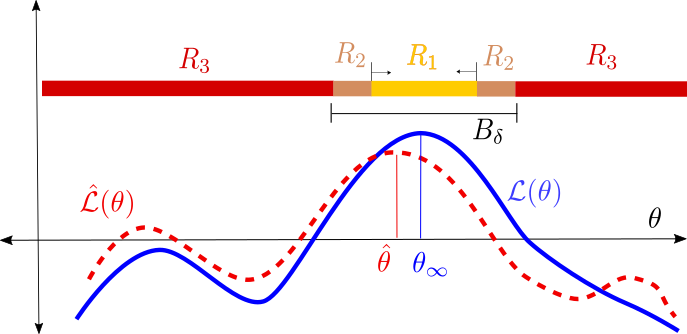
\includegraphics[width=\textwidth]{static_figures/BCLT_illustration.png}
\caption{Visual illustration of the proof technique.  As $N$ increases,
$\likhat(\theta) \rightarrow \lik(\theta)$
uniformly within $\thetaball{\delta}$, $\likhat(\theta)$ remains
bounded away from $\likhat(\thetatrue)$ outside of $\thetaball{\delta}$,
and the region $R_1$ that matters for the posterior shrinks at
a rate slightly slower than $1/\sqrt{N}$.}
\figlabel{proof_technique}
\end{figure}



Taking as given that the posterior concentrates in the shrinking region $R_1$,
we can fully characterize the posterior using Taylor series expansions within
the region $R_1$.  Our ability to form these Taylor series is guaranteed by the
differentiability conditions of \assuref{bayes_clt} \itemref{loglik_smooth} and
\defref{bclt_okay} \itemref{bclt_okay_as}.  Our ability to control the terms in
the Taylor series is guaranteed by uniform laws of large numbers (Chapter 19 of
\citet{van:2000:asymptotic}), which hold via \assuref{bayes_clt}
\itemref{loglik_ulln} and \defref{bclt_okay} \itemref{grad_op1}.

Finally, establishing that the posterior concentrates in $R_1$ requires separate
treatment of the region $R_2$, which is compact but adjacent to the region of
posterior concentration, and $R_3$, which encompasses the entire domain outside
of $\thetaball{\delta}$.  Thanks to uniform convergence within
$\thetaball{\delta}$, the region $R_2$ can be dealt with via Taylor expansions
and carefully choosing the shrinking rate of $R_1$.  However, the region $R_3$
requires a suite of additional assumptions to guarantee that the posterior does
not behave pathologically in the tails: namely, that $\likhat(\theta)$ remains
strictly bounded away from $\likhat(\thetatrue)$ (\assuref{bayes_clt}
\itemref{strict_opt}), that the prior is proper and bounded (\assuref{bayes_clt}
\itemref{prior_smooth,prior_proper}), and that average prior expectations of the
function of interest exist (\defref{bclt_okay} \itemref{prior_op1}).

We note that most of our assumptions about the prior (boundedness, propriety,
that certain prior expectations are bounded) serve only to establish that the
unbounded region $R_3$ does not contribute meaningfully to the posterior.
Inspection of the proof will reveal that weaker assumptions could also suffice,
at the cost of increased technical or notational complexity. For example, since
our analysis is asymptotic, one could assume only that the \emph{posterior}
satisfies \assuref{bayes_clt} \itemref{prior_smooth,prior_proper} and
\defref{bclt_okay} \itemref{prior_op1} with probability one after some finite
number of observations.  This posterior could then play the role of the prior in
the rest of the proof without modification.

In \appref{normal_example}, we verify our assumptions and prove the consistency
of the IJ covariance in the simple closed form example of inferring a univariate
normal mean with a misspecified variance.  This example, though simple, provides
intuition as well as a template for more complex settings.





\subsection{Data weights and the influence function}
\seclabel{data_weights}
In this section, we briefly connect the IJ covariance to some related
literature on local sensitivity, outlier detection, and
the von Mises calculus.  The connections are illuminated by the following
``weighted posterior expectation''
%
\begin{align}
    %
    \expect{\postw}{\g(\theta)} =
        \frac{
        \int_{\thetadom} g(\theta)
            \exp\left(N \meann \w_n \ell(\x_n \vert \theta) \right) \prior(\theta)
                            d\theta}
             {\int_{\thetadom}
             \exp\left(N \meann \w_n \ell(\x_n \vert \theta) \right) \prior(\theta)
             d\theta},
             \eqlabel{weighted_post}
    %
\end{align}
%
where $\wvec = (\w_1, \ldots, \w_N) \in \rdom{N}$ is a length--$N$ vector
of scalar--valued weights, one for each datapoint.  Comparing
\eqref{g_post} with \eqref{weighted_post}, we see that
$\expect{\postw}{\g(\theta)} = \expect{\post}{\g(\theta)}$ when
$\wvec = \onevec$, where $\onevec$ is the length--$N$ vector containing
all ones.  When we can apply the dominated convergence theorem to
exchange posterior integration and differentiation
(see, e.g., Theorem 1 of \citet{giordano:2018:covariances}), it follows that
%
\begin{align}
    \fracat{\partial \expect{\postw}{\g(\theta)}}{\partial \w_n}{\wvec = \onevec} =
    \cov{\post}{\g(\theta), \ell(\x_n \vert \theta)} = \frac{1}{N} \infl_n.
    \eqlabel{infl_deriv}
\end{align}
%
Our ``influence scores'' are thus the values of the
``empirical influence function'' of the statistical functional $\expect{\post}{\g(\theta)}$,
and our $\gcovij$ the classical IJ covariance estimator
(see, e.g., \citet{mises:1947:asymptotic,reeds:1976:thesis,efron:1982:jackknife,hampel:2011:robustbook}, or
\citet{serfling:1980:approximation} for a textbook treatment).  Equivalently,
the empirical influence function can be understood as an instance of
``local sensitivity analysis'' to perturbations of data weights
\citep{gustafson:1996:localposterior,giordano:2018:covariances}, which
motivates application of the empirical influence function
to a wider variety of problems than variance estimation.
The related literature is too large to survey here, but
some examples are cross--validation
\citep{koh:2017:blackboxinfluence,giordano:2019:swiss}, identification
of outliers \citep{pregibon:1981:logistic,mcculloch:1989:localbayesianmodelinfluence,belsley:1980:regression},
identification of influential subsets \citep{giordano:2026:amip1,giordano:2026:amip2},
and interpretation of Bayesian posteriors
\citep{thomas:2018:reconcilingcurvatureandis,iba:2023:wkernel}.  The
present work rigorously connects Bayesian posterior expectations to this
large literature, and we anticipate applications beyond variance estimation.

However, the interpretation of $\infl_n$ as a local approximation, together
with the form of \eqref{weighted_post}, provides a cautionary warning
in the Bayesian context.  Though our experiments of \secref{experiments}
motivate the IJ covariance estimator as a way to avoid pathologies associated
with MAP estimation, the most common use of MCMC is to integrate out
high--dimensional posterior parameters that do not obey a BCLT.  The following
simple argument suggests that the IJ covariance may not work in such a case,
even for parameters that do obey a BCLT marginally.

Suppose, for example, that $\theta$ is the concatenation of two sets of
parameters: a finite--dimensional set of ``global'' parameters $\gamma$, and a
high--dimensional set of ``local'' parameters, $\lambda$.  A common such example
is where $\gamma$ are ``fixed effects'' and $\lambda$ ``random effects'' in a
panel data setting, and the full parameter set is the concatenation $\theta =
(\gamma, \lambda)$ (see, e.g.~\citet[Chapter 7]{davidson:2004:econometric},
though in a Bayesian context the distinction between fixed and random effects is
not always meaningful \citep[Chapter 11]{gelman:2006:arm}).  Suppose that
$\cov{\post}{\gamma} = \ordlogp{N^{-1}}$ but $\cov{\post}{\lambda}$ remains
bounded away from zero.  Take $\g(\theta) = \gamma$. Differentiating
\eqref{infl_deriv} again with respect to $\w_n$ and applying the tower property
and delta method gives:
%
\begin{align}
    \fracat{\partial^2 \expect{\postw}{\gamma}}{\partial \w_n^2}{\wvec = \onevec} =
    % \expect{\post}{
    %     \gammabar \ellbar(\x_n \vert \gamma, \lambda)^2
    %     }
    % =
    \cov{\p(\gamma \vert \xvec)}{
        \gamma,
        \cov{\p(\lambda \vert \gamma, \xvec)}{\ell_n(\gamma, \lambda)}
    } + \ordlogp{N^{-2}}
    \eqlabel{resid_term}
\end{align}
%
% where for compactness we have written $\gammabar = \gamma - \expect{\post}{\gamma}$
% and $\ellbar(\x_n \vert \theta) = \ell(\x_n \vert \theta) - \expect{\post}{\ell(\x_n \vert \theta)}$
%
where the $\ordlogp{N^{-2}}$ term assumes that third--order posterior cumulants
of $\p(\gamma \vert \xvec)$ are $\ordlogp{N^{-2}}$, as they would typically be
for a posterior which concentrates at root $N^{-1/2}$. By the tower property,
the first derivative is also a posterior covariance with respect to  $\p(\gamma
\vert \xvec)$:
%
\begin{align}
    \fracat{\partial \expect{\postw}{\gamma}}{\partial \w_n}{\wvec = \onevec} =
    \cov{\p(\gamma \vert \xvec)}{
        \gamma,
        \expect{\p(\lambda \vert \xvec, \gamma)}{\ell(\x_n \vert \gamma, \lambda)}
    }.
    \eqlabel{global_local_first_order}
\end{align}
%
See \appref{weights_higher_order} for details on the derivation of
\eqref{resid_term,global_local_first_order}.


If the function $\gamma \mapsto \cov{\p(\lambda \vert \gamma,
\xvec)}{\ell_n(\gamma, \lambda)}$ does not vanish as $N \rightarrow \infty$, it
follows from \eqref{resid_term,global_local_first_order} that both the first and
second derivatives are posterior covariances of non--vanishing functions of
$\gamma$, and so of the same order as $N \rightarrow \infty$.  Since the second
derivative is of the same order as the first derivative, the empirical influence
function's linear approximation to provide a poor approximation even to the
effect of leaving out a single datapoint.

Note that this counterexample
does not contradict our results from \thmref{ij_consistent}: if a BCLT applies
to $\lambda$ as well as to $\gamma$, then $\cov{\p(\lambda \vert \xvec,
\gamma)}{\ell(\x_n \vert \gamma, \lambda)} = \ordlogp{N^{-1}}$ inside the
covariance of \eqref{resid_term}, and the second derivative is
$\ordlogp{N^{-2}}$, as suggested by \thmref{bayes_clt_main}.
%
This intuition is rigorously developed and supported using von Mises expansions
in \citet{giordano:2024:oldbayesij}, which at the time of writing is still in
progress.
In light of this example, and of the analysis of
\citet{giordano:2024:oldbayesij} for the high--dimensional regime, we recommend
caution when employing the IJ covariance estimator --- or any method depending
on the empirical influence function ---  in settings where a BCLT may not apply
to the full posterior $\post$.




\subsection{Related Work}\seclabel{related_work}
Several other papers have studied the estimation of frequentist variability of
posterior expectations.  \citet{efron:2015:frequentist} provides results similar
to ours, but is limited to the special case of exponential families. The
frequentist sampling variability of Bayesian posterior expectations under
misspecification is studied in \citet{kleijn:2012:bvm} from a theoretical point
of view, motivating the form of the sandwich covariance.
\Citet{huggins:2024:bayesbagparameter} derive a BCLT for the ``BayesBag''
posterior which combines both posterior and bootstrap uncertainty; we conjecture
that a minor modification of their proof would prove the consistency of the
bootstrap alone as an estimator of the limiting frequentist variance of a
posterior mean. See also \citet{huggins:2022:bayesbag} for a closely related
BCLT result in the context of model selection, as well as the same authors'
earlier work on arxiv, \citet{huggins:2020:bayesbag}.  Although the IJ
covariance does not provide bootstrap samples for use in BayesBag posteriors
directly, the IJ covariance could be used to estimate the bootstrap covariance
term that appears in the law of total covariance decomposition of the BayesBag
covariance (see the final, unnumbered equation in Section 2.3 of
\citet{huggins:2024:bayesbagparameter}). Both \citet{vehtari:2024:psis} and
\citet{lee:2017:frequentistbayesse} consider importance sampling estimates to
the effect of dropping datapoints, with \citet{lee:2017:frequentistbayesse}
explicitly considering estimation of frequentist variability of the posterior
under an assumption of correct specification. However, importance sampling
estimates of frequentist variability can be expected to have very low sampling
efficiency even in moderate dimensional problems, since frequentist re--sampling
is expected to produce changes of the posterior mean on the same order as the
posterior standard deviation (see Example 9.2 of \citet{owen:2014:mcbook}).
Furthermore, misspecification can result in frequentist sampling variances that
are different than the posterior variance, which can further degrade importance
sampling efficiency as a function of dimension (see Example 9.3 of
\citet{owen:2014:mcbook}).

Our key result, \thmref{bayes_clt_main} is distinguished from previous BCLT
results primarily by tracking the data dependence in the residual of the series
expansion, though we also differ from some classical work by admitting
misspecification.  Our method of proof hews closely to the classical BCLT proofs
found in  Chapter 10 of \citet{van:2000:asymptotic}, Theorem 1.4.2 of
\citet{ghosh:2003:bayesian}, and \citet{lehman:1983:pointestimation}, all of
which study the asymptotic regime for a single posterior quantity under the
assumption of correct specification.  A series expansion for posterior
expectations similar to \thmref{bayes_clt_main} is established by
\citet{kass:1990:posteriorexpansions}, under stricter differentiability
conditions than ours, and only for a single posterior quantity of interest,
which is (implicitly) assumed not to depend on the dataset. A number of recent
papers have, like us, studied the asymptotic behavior of finite--dimensional
Bayesian posteriors under misspecification, though without explicitly
controlling data dependence
\citep{kleijn:2006:misspecification,miller:2021:bclt,kasprzak:2022:laplace}.

Our work is an application of the classical IJ estimator, which has been
extensively studied in the frequentist literature, but which to the best of the
authors' knowledge has not been applied to Bayesian posterior expectations (see,
e.g., \citet{jaeckel:1972:infinitesimal}, \citet{efron:1982:jackknife},
\citet{shao:2012:jackknife}, \citet{efron:2014:estimation},
\citet{wager:2014:confidence},
\citet{peng:2021:biasconsistencyalternativeperspectives},
\citet{ghosal:2022:infinitesimaljackknifecombinationsmodels}).
As we discuss more explicitly in \secref{data_weights}, the IJ covariance can be
viewed as the first term in a von Mises expansion of the Bayesian posterior
(\citet{mises:1947:asymptotic}, \citet{reeds:1976:thesis},
\citet{serfling:1980:approximation}), though we prove consistency directly
rather than via a functional series expansion.
\Citet{giordano:2024:oldbayesij} prove consistency of the IJ for posterior
expectations using von Mises expansions directly under stronger theoretical
assumptions, using results from the present paper.

As we discuss in the introduction, IJ estimation can be thought of as a
particular measure of local data robustness --- specifically, robustness to
random resampling of the data. We make this connection even more explicit in
\secref{data_weights} below. Viewing IJ estimators as local data robustness
connects our work to a large literature on ``local case influence,'' which
refers to a broad class of techniques that using derivatives to approximate the
effect of a datapoint or datapoints on a statistic of interest.  Local case
influence is an idea with a long history in frequentist and Bayesian statistics.
The literature is too vast to review systematically here, but some notable
references include
\citet{belsley:1980:regression,cook:1977:detectionofinfluential,
cook:1982:residualsandinfluenceinregression, cook:1986:assessment,
kempthorne:1986:decision,kass:1989:approximatebayesiansensitivity,
carlin:1991:expectedutilityinfluence,
zhu:2007:perturbation,koh:2017:blackboxinfluence,
thomas:2018:reconcilingcurvatureandis}.
The relationship between posterior covariances and derivatives has been noted
numerous times in the Bayesian robustness literature (e.g.
\citet{diaconis:1986:bayesconsistency}, \citet{gustafson:1996:localposterior},
\citet{basu:1996:local}, \citet{efron:2015:frequentist},
\citet{giordano:2018:covariances}). As we note in \secref{bayes_clt},
consistency of the IJ requires a kind of uniform guarantee over a large number
of local approximations, but most of the local case influence work focuses on a
datapoint or a small set of datapoints. Notable exceptions include
\citet{giordano:2019:swiss} in the frequentist literature and
\citet{zhu:2012:bayesiancaseinfluence} in the Bayesian literature, though we
note that Theorem 2 of \citet{zhu:2012:bayesiancaseinfluence} is stated in terms
of a fixed set of dropped datapoints.

Following the posting of the present work on the arXiv, a number of interesting
subsequent papers have proposed extensions and variants and applications of the
Bayesian IJ. \Citet{nguyen:2024:sensitivitymcmcbasedanalysessmalldata} applies
the IJ to the adversarial data--dropping work of
\citet{giordano:2026:amip1,giordano:2026:amip2} in MCMC settings.
\Citet{iba:2023:wkernel} connects the IJ covariance to kernel methods, and
\citet{iba:2023:posteriorweighted} apply ideas closely related to the Bayesian
IJ covariance to information criteria and model selection.  Two papers,
\textcite{ji:2025:ValidStandardErrors2025,luo:2026:RobustStandardErrors2026},
have systematically evaluated the Bayesian IJ covariance for use in the social
sciences in the presence of model misspecification. We hope that our approach
continues to motivate and inform connections between the frequentist and
Bayesian case influence literature.






%%%%%%%%%%%%%%%%%%%%%%%%%%%%%%%%%%%%%%%%%%%%%%%%%%%

\section{Experiments}
\seclabel{experiments}
We present two experimental analyses of the IJ covariance.  The first is a
simulated random effects model under misspecification.  We designed the
simulation to have a degenerate MAP approximation but well-behaved MCMC
posterior expectation, and show that the IJ covariance is able to accurately
estimate the true sampling variance over new draws of the data. The second
experiment is an application of the IJ covariance to a large number of linear
and generalized linear models and datasets taken from \citet{gelman:2006:arm}.
On these real-world datasets a simulated ground truth is unavailable, so we
compare the IJ covariances to the much more computationally expensive bootstrap
estimated variance.

Additional experimental results can be found in
\appref{simple_examples_appendix}, including a number of closed--form examples,
as well as an additional application to a real-world ``multilevel regression and
post--stratification'' analysis from the surveys literature
\citep{park:2004:mrp}.


\subsection{A degenerate joint MAP approximation with simulated data}
\applabel{singular_example}
As we describe in \secref{three_methods}, the IJ covariance is particularly
well-motivated in settings when the MAP $\thetahat$ is either unavailable or
unreliable, and one must turn to MCMC to integrate out a large number of
nuisance parameters.  In this section we present a simple simulated example of
such a case.
% A similar example on a real dataset can be found in PUT IN PILOTS
% can be found in REF APPENDIX.

Consider the following simple random effects model with responses. For the data,
we assume we have responses $y_n \in \rdom{}$, regressors $r_n \in \rdom{}$, and
group indicator vectors $z_n \in \{0, 1\}^K$, for $n=1,\ldots,N$ and some fixed
number of groups $K$.  We assume that all three are conditionally IID, so $\x_n
= (y_n, r_n, z_n)$, and draw according to the model
%
\begin{align}
\varepsilon_n \indep \normdist(\cdot \vert 0, 1)
\quad\quad
r_n \indep \normdist(\cdot \vert 0, 1)
\quad\quad
y_n = r_n + r_n^2 \varepsilon_n.\eqlabel{simple_sim_dgp}
\end{align}
%
In our experiments we used $K = \simNumRe$ and $N = \simNumObs$.

Suppose we now form a misspecified model of this data. Define the regression
parameter $\beta \in \rdom{}$, random effect vector $\mu \in \rdom{K}$, and
variances $\sigma_y^2$ and $\sigma_\mu^2$.  We will take the priors on $\mu_k$
to be independent given $\sigma_\mu$, and the priors on $\beta$, $\sigma_\y$ and
$\sigma_\mu$ to be diffuse; we will shortly be using the default diffuse priors
provided by \texttt{rstanarm}. Then we can model
%
\begin{align}\eqlabel{simple_sim_model}
%
y_n | z_n, r_n, \beta, \mu, \sigma_y^2 \indep&
    \normdist(\cdot | \beta r_n + z_n^T \mu, \sigma_y^2)
    \quad\textrm{ and }\quad
\mu_k | \sigma_\mu \indep
    \normdist(\cdot | 0, \sigma_\mu^2).
%
\end{align}
%
The model in \eqref{simple_sim_model} is misspecified because it does not model the
heteroskedasticity induced by $r_n^2 \varepsilon_n$ in \eqref{simple_sim_dgp}.
Note also that the group indicators $\z_n$ have no effect on the real data
generating process, and so estimates of very small $\sigma_\mu$ should be
supported by the data --- and the log likelihood should be degenerate at the
point $\sigma_\mu$, as we describe in detail below.

How good is the MAP estimate for this model?  The answer depends on which
variables are marginalized in the definition of $\theta$.  Suppose, for example,
we form the ``global'' MAP, optimizing over all the parameters,
including the random effects:
%
\def\badmap{\textrm{glob}}
\begin{align*}
%
\hat\beta^{\badmap}, \hat\sigma_y^{\badmap},
\hat\sigma_\mu^{\badmap}, \hat\mu^{\badmap} :=
    \argmax \ell(\xvec | \beta, \sigma_y, \sigma_\mu, \mu) +
            \log \pi(\mu | \sigma_\mu) +
            \log \pi(\beta, \sigma_y, \sigma_\mu).
%
\end{align*}
%
Optimizing over all parameters including the random effects is prone to
under-estimate the variance $\sigma_y$, particularly when $K$ is large relative
to $N$.  A simplified version of this phenomenon is the known as the
Neyman-Scott paradox \citep{freedman:2005:neymanscott}.  For this reason, one
does not typically optimize over $\mu$ for such a model.  Rather, one optimizes
the marginal posterior (or an approximation thereof):
%
\begin{align}\eqlabel{singular_map}
%
\hat\beta, \hat\sigma_y, \hat\sigma_\mu :=
    \argmax & \log \int p(\xvec | \beta, \sigma_y, \sigma_\mu, \mu)
        \pi(\mu | \sigma_\mu) d\mu  +
       \log \pi(\beta, \sigma_y, \sigma_\mu)
      \nonumber\\
= \argmax & \sum_{k=1}^K \ell(\xvec_k | \beta, \sigma_y, \sigma_\mu) +
\log \pi(\beta, \sigma_y, \sigma_\mu),
%
\end{align}
%
where $\xvec_k$ denotes $\{\x_n: z_{nk} = 1\}$, the observations in group $k$.
For Gaussian models such as this one, the needed integral in
\eqref{singular_map} can be computed in closed form. In the general case, there
exist non-MCMC methods such as marginal maximum likelihood estimation (MMLE) use
the Laplace approximation to approximate the integral
\citep{bates:2015:fitting}. However, it is possible to generate data $\xvec$ so
that even the MAP of \eqref{singular_map} estimates $\hat\sigma_\mu = 0$ for
sufficiently non-informative priors
\citep{chung:2012:avoiding,eager:2017:mixedterrible}.

In this case, we have designed the model and data generating process so that the
MMLE package \texttt{lme4} results in a numerically singular fit
($\hat\sigma_\mu = 0$) approximately half the time. When $\hat\sigma_\mu = 0$,
the second derivative of the log posterior is degenerate at the optimum, and
classical methods for approximating frequentist variances cannot be directly
applied.  In a random effects model for which even MMLE methods fail, MCMC is a
natural recourse. If an estimate of the frequentist variability of the posterior
mean is required, the IJ covariance is then a natural choice.


% Further, the heteroskedasticity in the residual
% variance, together with the modeling assumption of homoskedasticity, means that
% the Bayesian and frequentist covariances are expected to be different.


% In short, if we take $g(\theta) = \theta := \beta$ in this problem, then
% \eqref{nonsingular_map} gives us reason to believe that $\thetahat \approx
% \expect{\post}{\theta}$ and that both are approximately normally distributed,
% due to the concentration of the marginal log likelihood $\sumn \ell(\x_n |
% \theta)$.  However, we cannot easily compute the objective function or its
% derivatives, since $\ell(\x_n | \theta)$ involves an intractable integral.
% Nevertheless, we can run MCMC on all the parameters and use the IJ to
% approximate the frequentist variance of the limiting distribution of
% $\expect{\post}{\theta}$.  It is in precisely such cases that the IJ covariance
% is most useful.

\SingularResultsGraph{}

We simulated a single dataset for which the \texttt{lme4} fit happened to be
singular, and computed $\simNumMCMCDraws$ MCMC draws from the model of
\eqref{simple_sim_model} using \texttt{rstanarm}.  With these samples, we
computed the Bayesian posterior covariance and the IJ covariance.  We then
simulated $\simNumSims$ different datasets, ran the same MCMC procedure for
each, computed the posterior mean for each simulation, and computed the
covariance of the posterior means over the simulations.  Ideally, we expect the
IJ covariance to provide a good approximation to the simulation-based covariance
estimate.

The results are shown in \figref{simple_sim_result}.  As shown in the left plot,
the posterior variances of $\log \sigma_y$ and of $\beta$ are dramatically
less than the frequentist variances of $\expect{\post}{\log \sigma_y}$ and
$\expect{\post}{\beta}$.  The posterior of the log random effect variance, $\log
\sigma_\mu$, is extremely non-normal, and the IJ may not expected to perform
well, theoretically.  Nevertheless, we show that the IJ covariance is correct
despite the posterior variance being extremely inflated.

\subsection{Applied regression modeling examples}
\seclabel{arm_experiments}

We will now evaluate the performance of the IJ covariance on a number of
real-world models and datasets taken from \citet{gelman:2006:arm}.  We limited
our analysis to models for which data was available in the Stan examples
repository \citep{stan-examples:2017}, and for which \texttt{rstanarm}
\citep{rstanarm} was able to run in a reasonable amount of time. Since these are
real-world datasets, the ground truth sampling distribution is not available
from simulations, so, as an imperfect proxy, we compare the IJ covariance to the
(computationally expensive) bootstrap variance instead.

% What are our parameters of interest?
All models we considered from \citet{gelman:2006:arm} were instances of
generalized linear models, including both ordinary and logistic regression as
well as models with only fixed effects and models that include random effects.
Model details, including the number of estimated quantites of each type, are
given in \tabref{arm_models} of \appref{experiment_arm_appendix}.  For
parameters of interest, $g(\theta)$, we took all fixed-effect regression
parameters, the log of the residual variance (when applicable), and the log of
the random effect variance (when applicable). We did not examine random effects,
nor the random effect covariances for the few models with multiple random
effects, out of concern that a BCLT might not be expected to hold for these
parameters.  Below, when we refer to a ``parameter,'' we refer to a scalar
parameter of interest in a particular model for a particular dataset; there were
a total of $\armNumCovsEstimated$ such parameters.

For each model and dataset, we fix a number of MCMC samples, $M =
\armNumMCMCSamples$ to draw for each posterior sample, and a number of
bootstraps samples to draw, $B = \armNumBootstraps$. The total computation time
summed across all models for the initial MCMC and IJ computation was
$\armTotalMCMCTimeMins$ minutes, and the total bootstrap compute time summed
across all models and bootstrap samples was $\armTotalBootTimeHours$
hours.\footnote{Naively, one would expect the total bootstrap compute time to be
roughly $B = \armNumBootstraps$ times the compute time of the single MCMC run,
but the total bootstrap time was in fact longer than this. We conjecture that
the bootstrap time scaled super-linearly due to the fact that some bootstrap
samples led to posteriors that were less well-conditioned than the original
datasets, and so incurred more rejections during the MCMC procedure.}
%
For each parameter of interest, we use a single run of MCMC
to compute the IJ covariance estimate, $\gcovijhat$.  Using \algrref{boot}, we
draw $B$ different bootstrap samples, compute $M$ MCMC samples for each, and
finally compute the bootstrap variance estimate, $\gcovboothat$.

All together, this procedure produces comparisons between $\armNumCovsEstimated$
distinct covariance estimates from $\armNumModels$ different models using
$\armNumDatasets$ distinct datasets. The median number of observations amongst
the models was $\armMedianNumObs$, and the range was from $\armMinNumObs$ to
$\armMaxNumObs$ exchangeable observations.  Since we fit our models in
\texttt{rstanarm}, we were able to use the function \texttt{rstanarm::log\_lik}
to compute $\ell(\x_n \vert \theta)$, so $\gcovijhat$ required essentially no
additional coding.  We used the default priors provided by \texttt{rstanarm}.




\ARMGraphDiff{}


\ARMGraphZ{}


% Why do we need summary metrics
With $\armNumCovsEstimated$ covariances to report, we must summarize our results
into a few model--agnostic high-level accuracy summaries.  To this end, for each
parameter $j$ in each model $i$, we computed the following measure of both the
``practical significance'' and ``statistical significance'' of the IJ covariance
covariance as a proxy for the bootstrap variance:
%
\begin{align}
%
\normdiffij_{ij} :=
     \frac{\gcovijhat_{ij} - \gcovboothat_{ij}}
     {\left| \gcovboothat_{ij} \right| + \seboot_{ij}}
\quad\textrm{and}\quad
\zdiff_{ij} :=
\frac{\gcovijhat_{ij} - \gcovboothat_{ij}}
     {\sqrt{(\seij_{ij})^2 + (\seboot_{ij})^2}}.
\eqlabel{arm_metrics}
%
\end{align}
%
In \eqref{arm_metrics}, the quantities $\seij$ and $\seboot$ are measures of
the Monte Carlo error in the corresponding covariance estimates
(see \appref{experiments_sampling_error} for details).

The metric $\normdiffij_{ij}$ is a (noisy) measure of the proportional
difference between $\gcovijhat_{ij}$ and $\gcovboothat_{ij}$. The term
$\seboot_{ij}$ is included to retain a meaningful notion of scale when
$\gcovboothat_{ij}$ is nearly zero due to chance alone.
%
The metric $\zdiff_{ij}$ is the z-statistic which we would compute to test
equality between $\gcovijhat_{ij}$ and $\gcovboot_{ij}$ using our estimates of
the sampling error.  Despite this interpretation, the z-statistics for different
parameters within a given model are based on the same MCMC samples and so are
not independent, and we should be cautious in interpreting the collection of
$\zdiff_{ij}$ as the basis of any kind of formal hypothesis test. Rather, we
recommend thinking of $\zdiff_{ij}$ as heuristics whose marginal distributions
summarize the error $\gcovijhat - \gcovboot$ relative to Monte Carlo error.


% \footnote{Note that the relative errors $\normdiffij$ and
% $\normdiffbayes$ do not attempt to remove or account for Monte Carlo error.  One
% might imagine computing the relative error after deconvolving the Monte Carlo
% error and covariance estimates using, say, nonparametric empirical Bayes.  We
% investigated such an approach, but the resulting procedure was complicated and
% the results qualitatively similar to \figref{normerr_graph} below, so we will
% report only the relatively simple metrics $\normdiffij$ and $\normdiffbayes$.}
%
The distributions of $\normdiffij_{ij}$ and $\zdiff_{ij}$ across models,
datasets, and parameters are shown in \figref{normerr_graph,relerr_graph}
respectively.
%
For models with more data, the IJ provides a reasonable approximation to the
much more computationally expensive bootstrap, with roughly half of the IJ
covariance estimates falling well within 50\% of the bootstrap covariance
estimates, and rejecting the hypothesis test of equivalence at roughly the
nominal rate.  For models with less data, IJ estimates do not appear to
systematically deviate from the bootstrap estimates, but are more variable.
Recall that we expect, theoretically, only that the IJ and bootstrap variances
coincide as $N \rightarrow \infty$.

The distribution of $\zdiff_{ij}$ suggests that the apparent differences between
the IJ and bootstrap can be accounted for by Monte Carlo error alone in the
large models but not necessarily the small ones.  Recalling that both the
bootstrap and the IJ covariances are distinct approximations of the same
quantity which are close to one another only asymptotically, we conjecture that
the needed asymptotics have not yet kicked in for models with fewer datapoints.

% In \appref{experiment_arm_appendix}, we show that the Bayesian posterior
% covariance is a poor approximation for the bootstrap in larger datasets,
% particularly for covariances involving at least one scale parameter. We
% conjecture that the gap between the IJ covariance and the posterior covariance
% for log scale parameters may be driven by misspecification, though a more
% careful investigation is beyond the scope of the present work.



%%%%%%%%%%%%%%%%%%%%%%%%%%%%%%%%%%%%%%%%%%%%%%%%%%%

\section{Conclusion}
We define and analyze the IJ covariance estimate of the frequentist variance of
Bayesian posterior expectations.  The IJ covariance is computationally
appealing, since it can be computed easily from only a single set of MCMC draws,
in contrast to the bootstrap, which, in general, requires many distinct MCMC
chains.  In finite dimensional problems obeying a central limit theorem, we show
that the IJ covariance is consistent, since it consistently estimates the
sandwich covariance.  Our work rigorously connects Bayesian posterior inference
with a large and growing literature on applications of the empirical influence
function.

We caution that our proofs are asymptotic, based on finite-dimensional
posteriors, and unfortunately come with no accompanying guarantees for any
particular dataset.  Based on our experience, we are confident recommending the
IJ covariance as a rough but computationally efficient check for worryingly high
levels of frequentist sampling variance. However, in applications where precise
frequentist coverage is crucial, we recommend supplementing the IJ covariance
with more computationally expensive procedures such as the bootstrap or
conformal intervals \citep{huggins:2022:bayesbag,fong:2021:conformal}.
Furthermore, as we discuss in \secref{data_weights} above, a simple argument
suggests that the IJ covariance will be inaccurate in high-dimensional
posteriors, and the IJ should be used with extreme caution in such cases.
Forming diagnostics to alert the user when IJ covariance may be inaccurate is an
exciting and important avenue for future work.

\notbool{blind} { 
    \section{Acknowledgements}
    We are grateful for conversations with Jeffrey Miller, Jonathan Huggins, Tin
Nguyen, Peter Bickel, Wesley Johnson, and Miko\l{}aj Kasprzak, as well as to the
anonymous reviewers for their valuable comments and suggestions.  This research
was supported in part by an ONR Early Career Grant and an NSF CAREER Award.
}

\section{Data Availability Statement}


A complete copy of the code and data needed to reproduce our
experiments can be found in the github repository
\ifbool{blind} {
    \texttt{(ANONYMIZED)}
} {
    \url{https://github.com/rgiordan/BayesIJPaper}
}
and in the paper's supplementary material,


\printbibliography{}

%%%%%%%%%%%%%%%%%%%%%%%%%%%%%%%%%%%%%%%%%%%%%%%%%%%

\ifbool{arxiv} {
    \newpage
    \section*{The Bayesian Infinitesimal Jackknife for Variance: Supplemental information and proofs}
    


%%%%%%%%%%%%%%%%%%%%%%%%%%%%%%%%%%%%%%%%%%%%%%%%%%%
%%%%%%%%%%%%%%%%%%%%%%%%%%%%%%%%%%%%%%%%%%%%%%%%%%%
% Appendices
%%%%%%%%%%%%%%%%%%%%%%%%%%%%%%%%%%%%%%%%%%%%%%%%%%%
%%%%%%%%%%%%%%%%%%%%%%%%%%%%%%%%%%%%%%%%%%%%%%%%%%%


\section*{The Bayesian Infinitesimal Jackknife for Variance: Supplemental information and proofs}
\appendix

\section{A simple closed-form example}
\applabel{normal_example}
\def\thetagen{\theta_{\mathrm{True}}}
\def\xbar{\tilde{\x}}

In this section, we illustrate verification of our assumptions and the
consistency of the IJ covariance with a simple closed form example, that of
inferring a univariate normal mean with a misspecified variance. More elaborate
examples can be found in \appref{simple_examples_appendix}, including a Poisson
model in the presence of overdispersed data and multilinear regression in the
presence of heteroskedasticity.

For some fixed $\thetagen \in \rdom{}$ and $\sigma^2 \ne 1$, let us
consider the following data generating process and model:
%
\begin{align*}
%
\textrm{Data generating process:}\quad&&
x_n &\iid \normdist(\cdot | \thetagen, \sigma^2) \\
\textrm{Model:}\quad&&
x_n \vert \theta &\iid \normdist(\cdot | \theta, 1) &
\theta &\sim \normdist(\cdot | 0, 1).
%
\end{align*}
%
We will take $\theta$ to be our quantity of interest, so $\g(\theta) = \theta$.
Since $\sigma^2 \ne 1$ the model is misspecified, and so we expect the posterior
variance $\cov{\post}{\theta}$ to differ from $\gcovtrue$, even asymptotically.

For this simple model, the posterior is available in closed form:
%
\begin{align*}
    \post = \normdist\left( \theta \vert \xbar, (N + 1)^{-1} \right)
    \quad\textrm{where}\quad
    \xbar :={} \frac{1}{N+1} \sumn \x_n.
\end{align*}
%
From this, we can see that $\thetatrue = \lim_{N \rightarrow \infty}
\expect{\post}{\theta} = \thetagen$, It happens in this simple example that
$\thetatrue$ is ``consistent'' for the true mean $\expect{\fdist(\xn)}{\xn}$,
though in general this need not be the case.  For example, the model's trivial
``estimate'' of $\var{\fdist(\xn)}{\xn}$ is $1$, which is never equal to the
true value of $\sigma^2$.

One can readily verify that \assuref{bayes_clt,bclt_okay} are satisfied for this
model and this particular value of $\thetatrue$. Arguably the most challenging
condition is the final part of \assuref{bayes_clt} \itemref{strict_opt}, which
one can show via strong convexity of the log likelihood, together with
convergence of $\frac{1}{N} \sumn \ellgrad{1}(\x_n \vert \thetatrue) \plim 0$ by
the ordinary law of large numbers.  Using special structure of a particular
problem (like strong convexity) to establish a condition like
\assuref{bayes_clt} \itemref{strict_opt} is common in the literature --- see,
for example, textbook proofs of the consistency of M-estimators on unbounded
domains (e.g.~Theorem 9.11 of \citet{keener:2010:theoretical} or Chapter 6.2 of
\citep{huber:2011:robust}).

We begin by establishing \corref{bayes_expectation_dist} and identifying our target,
$\gcovtrue$. By the ordinary CLT applied to our closed-form expression for
$\expect{\post}{\theta}$, we have that
$$
\sqrt{N}\left(\expect{\post}{\theta} - \thetatrue\right) \dlim
\normdist\left(\cdot \vert 0, \sigma^2 \right),
$$
from which we see that $\gcovtrue = \sigma^2$.  It happens, in this case, that
the variance of the limiting distribution is also the limit of the variance,
since
$$
N \var{\xfdist}{\expect{\post}{\theta}} =
    \frac{N^2}{(N+1)^2}\sigma^2 \rightarrow \sigma^2 \gcovtrue.
$$
The asymptotic equivalence between the variance of the limit and the limit of
the variance occurs in this case because $\var{\xfdist}{\expect{\post}{\theta}}$
is uniformly integrable as a sequence in $N$ (Theorem 10.3.6 of
\citet{dudley:2018:realanalysis}).  We emphasize, however, that our theorems do
not assume uniform integrability, and we aim to estimate the variance of the
limiting normal distribution, not the limiting value of the variance, as
discussed in the text surrounding \eqref{gtrue}.

To complete \corref{bayes_expectation_dist}, we need to show that the expression
for $\gcovtrue$ is correct. In this case, $\ggrad{1}(\theta) = 1$, and the
remaining quantities are (up to constants not depending on
$\theta$):
\begin{align}
%
\likhat(\x \vert \theta) ={}&
    -\frac{1}{2N} \sumn \left(x_n^2 - 2x_n \theta + \theta^2\right) + \textrm{Constant}
\quad\textrm{and}\quad
% \nonumber\\
\log \pi(\theta) ={}& -\frac{1}{2}\theta^2 + \textrm{Constant} \Rightarrow \nonumber \\
\thetahat ={}& \xbar
\quad\textrm{,}\quad
\ellgrad{1}(\x \vert \theta) ={} x_n - \theta
\quad\textrm{and}\quad
\likhatk{2}(\x \vert \theta) ={} -1 \Rightarrow \nonumber \\
\scorecovhat ={}& \meann \left(x_n - \xbar\right)^2
\quad\textrm{,}\quad
\infohat ={} 1
\quad\textrm{and}\quad
\gcovhat ={} \infohat^{-1} \scorecovhat \infohat^{-1} = \scorecovhat.
\eqlabel{normal_gcovhat}
%
\end{align}
%
It is readily verified that $\scorecovhat \plim \sigma^2 = \gcovtrue$,
so we have verified the conclusion of \corref{bayes_expectation_dist}.

Finally, we manually verify \thmref{ij_consistent}. The influence score is given by:
%
\begin{align*}
%
\infl_n ={}& N \cov{\post}{
    \theta, -\frac{1}{2} \left(\x_n^2 - 2\x_n \theta + \theta^2 \right)} \\
={}&
 -\frac{1}{2}  N \cov{\post}{\theta, 1} \x_n^2 +
 N \cov{\post}{\theta, \theta} \x_n  + N  \cov{\post}{\theta, \theta^2}
={} \frac{N}{N+1} \x_n + \textrm{Constant},
%
\end{align*}
%
where the constant in the final line is the same for all $\x_n$.  Since the IJ covariance
depends only on the difference $\infl_n - \bar{\infl}$, quantities that are the
same for each $n$ can be neglected in the IJ covariance computation. Therefore
the IJ covariance estimate is given by
%
\begin{align*}
%
\gcovij ={}& \meann \left(\infl_n - \bar{\infl} \right)^2
={} \frac{N^2}{(N + 1)^2} \scorecovhat \plim \sigma^2 = \gcovtrue.
%
\end{align*}
%
Thus $\gcovij$ differs from the $\gcovhat$ given in \eqref{normal_gcovhat} by a
factor that vanishes asymptotically.  So, like $\gcovhat$, $\gcovij$ is a
consistent estimator of the asymptotic variance $\gcovtrue$.


%%%%%%%%%%%%%%%%%%%%%%%%%%%%%%%%%%%%%%

\section{Notation key}
For ease of reference, we provide here a table of key quantities
defined and used through the course of our proofs.

\begin{table}[!h]
\begin{tabular}{|c|c|c|}
\hline
Symbol & Description & Definition \\
\hline
$\infl_n$ & Influence score of the $n$--th observation & \eqref{ij_terms}\\
\hline
$\indexset$ & A set of sets of data indices & \defref{index_sets} \\
\hline
$\xvec_s$ & The observations corresponding to $s \in \indexset$ & \defref{index_sets} \\
\hline
$\phi(\theta, \xvec_s)$ &
    A function of interest depending on $\theta$ and a set of datapoints &
    \defref{bclt_okay_index} \\
\hline
$\thetaball{\delta}$ & A $\delta$-ball around $\thetatrue$ & \assuref{bayes_clt} \\
\hline
$\tresid{k}{\phi, \thetahat, \theta}$ & The $k$--th order Taylor series residual term for $\phi$ &
    \defref{taylor_residual} \\
\hline
$\normhatarg{\tau}$ & Gaussian density with covariance $\infohat^{-1}$  & \defref{gaussian_defs} \\
\hline
$\normresid{\lambda}{S}(\tau)$ &
    Isotropic Gaussian density with precision $\lambda$ truncated to set $S$ &
    \defref{gaussian_defs} \\
\hline
$\normalizer$ & Normalizing constant for $\normhatarg{\tau}$& \defref{gaussian_defs} \\
\hline
$\infoev,\infoevhat$ & Minimum eigenvalues of $\info$, $\infohat$ & \defref{loglik_details_def} \\
\hline
$\tau$ & Centered and scaled parameter $\sqrt{N}(\theta - \thetahat)$ & \eqref{tau_defn} \\
\hline
$R_1,R_2,R_3$ & Inner, middle, and outer regions of integration & \defref{region_division} \\
\hline
$\delta_1$ & Scale of boundary between $R_1$ and $R_2$ & \defref{region_division} \\
\hline
$\delta_2$ & Scale of boundary between $R_2$ and $R_3$ & \defref{region_division} \\
\hline
$I(\phi)$ & The integration functional of $\phi$ & \eqref{integral_funcational} \\
\hline
$I_k(\phi)$ & Integration functional restricted to region $R_k$ &
    \eqref{region_integration_functional} \\
\hline
$\regevent$ & The event that the problem is ``regular'' & \lemref{regular_event} \\
\hline
$\epsilon_U$ & Arbitrarily small accuracy parameter for the regular event & \lemref{regular_event} \\
\hline
$\epsilon_L$ & Log likelihood lower bound in regular event & \lemref{regular_event} \\
\hline
$\resid{\phi}(\xvec_s)$ & The BCLT residual for $\expect{\post}{\phi(\theta, \xvec_s)}$ &
    \defref{bclt_resid} \\
\hline
$\resid{k}(\xvec_s)$ & The $k$--th component of the BCLT residual & \defref{bclt_resid} \\
\hline
\end{tabular}
\caption{Notation key}\label{tab:notation_key}
\end{table}


\section{Setup and Preliminaries}

\subsubsection{Derivative arrays}


Throughout our proofs, we will be forming and manipulating higher-order
Taylor expansions of functions of $\theta$.  The arrays of derivatives
in these expressions will always be summed against a direction, typically
$\tau = \sqrt{N}(\theta - \thetahat)$.  In order to avoid cumbersome
summation notation for all such terms, we will implicitly sum derivative arrays
against $\tau$ or $\theta$.  or example, for
a function $\psi(\theta, \x_n) \in \rdom{D_\psi}$, we will write
%
\begin{align*}
\psigrad{3}(\thetahat, \x_n)\tau^3 =
\sum_{a=1}^D \sum_{b=1}^D \sum_{c=1}^D
    \fracat{\partial^3 \psi(\theta, \x_n)}
           {\partial\theta_{a} \partial\theta_{b} \partial\theta_{c}}
           {\thetahat} \tau_{a} \tau_{b} \tau_{c}.
\end{align*}
%
Occasionally we will need to sum several derivative arrays against $\tau$,
particularly in \secref{region_r1}.  Since the directions $\tau$ will always be
the same, we will combine the $\tau$ in such expressions with no ambiguity. For
example, for the term involving $\likhatk{3}(\thetahat)$ in the statement of
\thmref{bayes_clt_main}, we will write
%
\begin{align*}
%
\psigrad{1}(\thetahat, \x) \likhatk{3}(\thetahat) \tau^4 =
\sum_{a=1}^{D} \sum_{b=1}^{D} \sum_{c=1}^{D} \sum_{d=1}^{D}
    \psigrad{1:a}(\thetahat, \x) \likhatk{3:b,c,d}(\thetahat)
    \tau_a \tau_b \tau_c \tau_d.
%
\end{align*}
%

When necessary, higher
derivatives will be indexed in the parentheses.  For example,
$\psigrad{2:i,j}(\theta, \x_n)$ will denote the length--$D_\psi$ vector
%
\begin{align*}
%
\fracat{\partial^2 \psi(\theta, \x_n)}
    {\partial\theta_i \partial\theta_j}{\theta, \x_n}.
%
\end{align*}
%
%\end{defn}

We denote by $\ind{A}$ the indicator function taking value $1$ when the
event $A$ occurs and $0$ otherwise.

% Order notation
We will use order notation to describe the behavior of quantities as $N
\rightarrow \infty$.  For example, we will use $z = O(\phi(N))$ to mean there
exists an $N^*$ and an $A > 0$ such that $N > N^* \Rightarrow z < A \phi(N)$. In
our notation, $A$ and $N^*$ in this definition will never depend on the data,
$\xvec$, though they may depend on unobserved population quantities.
%
Dependence on the data $\xvec$ in order notation will always be represented with
$O_p$ notation.  For example, $z = O_p(\phi(N))$ will mean that there exists an
$A > 0$ such that for any $\epsilon > 0$, there is a corresponding $N^*$ and
such that
%
\begin{align*}
%
N > N^* \quad\Rightarrow\quad
    \expect{\xfdist}{\ind{z < A \phi(N)}} > 1 - \epsilon.
%
\end{align*}
%
Here, $A$ does not depend on $\epsilon$.  The meaning is that the event $z =
O(\phi(N))$ occurs with arbitrarily high probability as $N$ goes to infinity.
The notation $\tilde{O}$ and $\tilde{O}_p$ will have the same meaning as $O$ and
$O_p$ notation respectively, but with factors of $\log N$ possibly ignored.


\subsubsection{General index sets}\seclabel{index_sets}

%%%%%%%%%%%%%%%%%%%%%%%%%%%%%%%%%%%%%%%%%%%%%%%%%%%%%
% Index sets

To succinctly state our theorems for double sums, it will be convenient to
introduce a more general index notation.

\begin{defn}\deflabel{index_sets}
    %
    Let $\indexset$ denote a set of sets of data indices, where each member $s \in
    \indexset$ has the same cardinality, and for $s \in \indexset$, let $\xvec_s$
    denote the set of corresponding datapoints.  We write $\phi(\xvec_s)$ for a
    function that depends on $|s|$ datapoints.  For example, if $\indexset = \{1,
    \ldots, N \} =: [N]$, then $\xvec_s = \x_s$, and $\means \phi(\xvec_s) = \meann
    \phi(\x_n)$.  Similarly, if $\indexset = [N] \times [N]$, then $\xvec_s =
    (\x_{s_1}, \x_{s_2})$, and $\means \phi(\xvec_s) = \frac{1}{N^2} \sum_{n=1}^N
    \sum_{m=1}^N \phi(\x_n, \x_m)$.
    %
\end{defn}

We now state a generalization of \defref{bclt_okay} that applies to 
generic index sets as defined in \defref{index_sets}.

\begin{defn}\deflabel{bclt_okay_index}
%
For an index set $\indexset$, a data-dependent function
$\phi(\theta, \xvec_s)$ is $K$-th order BCLT-okay if,
for each $k = 1, \ldots, K$,
%
\begin{enumerate}
%
\item\itemlabel{bclt_okay_as_index}
    $\theta \mapsto \phigrad{k}(\theta, \xvec_s)$ is BCLT-okay
    $\fdist$-almost surely
%
\item\itemlabel{prior_op1_index}
    $\means \expect{\prior(\theta)}{\norm{\phi(\theta, \xvec_s)}^2_2} = O_p(1)$.
%
\item\itemlabel{grad_op1_index}
For some $\delta > 0$,
$\sup_{\theta \in \thetaball{\delta}}
    \means \norm{\phigrad{k}(\theta, \xvec_s)}^2_2 = O_p(1)$.
%
\end{enumerate}
%
\end{defn}


Note that a function is BCLT--okay according to \defref{bclt_okay} precisely if
it is BCLT--okay according to \defref{bclt_okay_index} with index set $\indexset
= [N]$.  Although $\indexset = [N]$ and $\indexset = [N]\times[N]$ will be the
only examples of $\indexset$ we will use in the present paper, we believe it is
clearer to keep the notation general.   

In particular, \thmref{bayes_clt_main} is stated in terms of $\indexset = [N]$,
but we will prove that it holds for generic index sets of the form
\defref{bclt_okay_index}.  Formally, we will prove \thmref{bayes_clt_main} under
the following \assuref{core_bclt_assu}, noting that \assuref{core_bclt_assu} is
assumed by \thmref{bayes_clt_main} for $\indexset = [N]$.

\begin{assu}\assulabel{core_bclt_assu}
%
Assume that $\phi(\theta, \xvec_s)$ is third-order BCLT-okay
according to \defref{bclt_okay_index}, and that \assuref{bayes_clt} holds.
%
\end{assu}


\subsection{Taylor series expansions and their asymptotics}\applabel{loglik_asymptotics}
The proofs below repeatedly rely on two key ideas: Taylor series
expansions, and uniform asymptotic control on the terms that arise.
In this section, we introduce these ideas and prove two key
lemmas.  The first, \lemref{taylor_residual}, gives the form
of a Taylor series expansion.  The second, \lemref{ulln},
controls the asymptotic behavior of the log likelihood
and its derivatives in a neighborhood of $\thetatrue$.


%%%%%%%%%%%%%%%%%%%%%%%%%%%%%%%%%%%%%%%%%
%%%%%%%%%%%%%%%%%%%%%%%%%%%%%%%%%%%%%%%%%
%%%%%%%%%%%%%%%%%%%%%%%%%%%%%%%%%%%%%%%%%


\subsubsection{Taylor series expansions}

Our analysis is based strongly on Taylor series expansions.
We will use the following two minor variants of standard analysis tools.
The first is a multivariate version of the integral form of the Taylor series
residual for a vector-valued function.

\begin{defn}\deflabel{taylor_residual}
%
For a $k$-times differentiable function $\phi(\theta)$, a fixed $\thetahat$, and
and $\theta$, define the residual functional
%
\begin{align*}
%
\tresid{k}{\phi, \thetahat, \theta} :=
    \frac{1}{(k-1)!} \int_0^1 (1 - t)^{k-1}
        \phigrad{k}(\thetahat + t (\theta - \thetahat)) dt.
%
\end{align*}
%
\end{defn}
%
The residual $\tresid{k}{\phi, \thetahat, \theta}$ is an array of the same
dimension as the $k$-th order derivative, $\phigrad{k}(\theta)$.  Observe that,
for any norm $\norm{\cdot}$,
%
\begin{align*}
    %
    \norm{\tresid{k}{\phi, \thetahat, \theta}} \le
        \frac{1}{(k-1)!} \sup_{\thetatil: \norm{\thetatil - \thetahat}_\infty \le
                                          \norm{\theta - \thetahat}_\infty}
                            \norm{\phigrad{k}(\thetatil)}.
    %
\end{align*}
%
\begin{lem}\lemlabel{taylor_residual}
%
A $K$-times continuously differentiable function $\phi(\theta)$ has Taylor
series residual
%
\begin{align*}
\phi(\theta) =
    \sum_{k=0}^{K-1} \frac{1}{k!} \phigrad{k}(\thetahat) (\theta - \thetahat)^k +
    \tresid{K}{\phi, \thetahat, \theta} (\theta - \thetahat)^K.
\end{align*}
%
\begin{proof}
%
Let $\phi_d(\theta)$ denote the $d$-th component of the vector $\phi(\theta)$
(contrast this notation with for the $d$-th order derivative
$\phigrad{d}(\theta)$). Consider the scalar to scalar map $t \mapsto
\phi_d(\thetahat + t (\theta - \thetahat))$. Taking the integral remainder form
of the $K - 1$-th order Taylor series expansion of this scalar map
\cite[Appendix B.2]{dudley:2018:analysis} and stacking the result into a vector
gives the desired result.
%
\end{proof}
%
\end{lem}



%%%%%%%%%%%%%%%%%%%%%%%%%%%%%%%%%%%%%%%%%
%%%%%%%%%%%%%%%%%%%%%%%%%%%%%%%%%%%%%%%%%
%%%%%%%%%%%%%%%%%%%%%%%%%%%%%%%%%%%%%%%%%

\subsubsection{Log likelihood asymptotics}

To use \lemref{taylor_residual} to study $\likhat(\theta)$, we will need to
expand \defref{loglik_def} with the following quantities.

%%%%%%%%%%%%%%%%%%%%%%%%%%%%%%%%%%%%%%%%
%%%%%%%%%%%%%%%%%%%%%%%%%%%%%%%%%%%%%%%%
\begin{defn}\deflabel{loglik_details_def}
\begin{align*}
%
\likhatk{k}(\theta) :={}&
   \frac{1}{N} \sumn \ellgrad{k}(\x_n \vert \theta) +
    %\frac{1}{N} \frac{\prior_{(k)}(\theta)}{\prior(\theta)} % NOT CORRECT
    \frac{1}{N} \logpriorgrad{k}(\theta)
&
\likk{k}(\theta) :={}& \int \ellgrad{k}(\xn \vert \theta) d\fdist(\xn)
\\
\infoev :={}& \textrm{The minimum eigenvalue of }\info &
\infoevhat :={}& \textrm{The minimum eigenvalue of }\infohat
%
\end{align*}
%
Note that, following our convention, $\likhatk{k}(\theta)$ is the $k$--th
partial derivative of $\likhat(\theta)$ with respect to $\theta$.

The term $\likk{k}(\theta)$ is a potential abuse of notation, since it is only
the partial derivative of $\lik(\theta)$ under the assumption that we can
interchange integration and differentiation.  Though we will in fact be assuming
sufficient conditions for this interchange (\assuref{bayes_clt}
\itemref{loglik_ulln}), our proofs will simply use the above definition of
$\likk{k}(\theta)$ directly.
\end{defn}
%
Using \lemref{taylor_residual}, we can then form a Taylor series expansion
around $\thetahat$, an expression that we will analyze carefully in
\appref{bayes_clt_proof}:
%
\begin{align}
\likhat(\theta) ={}&
    \likhat(\thetahat) +
    \likhatk{1}(\thetahat)(\theta - \thetahat) +
    \frac{1}{2}\likhatk{2}(\thetahat)(\theta - \thetahat)^2 +
\nonumber
\\&
    \frac{1}{6}\likhatk{3}(\thetahat)(\theta - \thetahat)^3 +
    \tresid{4}{\likhat, \thetahat, \theta} (\theta - \thetahat)^4.
    \eqlabel{loglik_series_example}
\end{align}
%

We now turn to the task of controlling the kinds of terms that arise in
\eqref{loglik_series_example}. One of our key tools in the proof of
\lemref{ulln} will be \emph{uniform laws of large numbers} (ULLNs), a concept
which we make concrete in \defref{ulln}. Typically, ULLNs require that the
sample average $\meann \phi(\x_n, \theta)$ converge to
$\expect{\fdist(\xn)}{\phi(\x_n, \theta)}$ uniformly over $\theta$ in some
compact set.
%
%%%%%%%%%%%%%%%%%%%%%%%%%%%%%%%%%%%%%%%%%%%%%
%%%%%%%%%%%%%%%%%%%%%%%%%%%%%%%%%%%%%%%%%%%%%
\begin{defn}\deflabel{ulln}
%
Recall the definition of $\thetaball{\delta}$ from \assuref{bayes_clt}. We say a
``uniform law of large numbers'', or ``ULLN'', holds for a function
$\phi(\theta, \xn)$ if, for some $\delta > 0$,
%
\begin{align*}
%
\sup_{\theta \in \thetaball{\delta}}
\norm{\meann \phi(\theta, \x_n) -
\expect{\fdist(\xn)}{\phi(\theta, \xn)}}_2
\plim 0,
%
\end{align*}
%
where $\expect{\fdist(\xn)}{\phi(\theta, \xn)}$ is finite.
%
\end{defn}
%%%%%%%%%%%%%%%%%%%%%%%%%%%%%%%%%%%%%%%%%%%%%

In general, a ULLN requires that the set of functions $\left\{\theta \mapsto
\phi(\theta, \xvec): \norm{\theta - \thetatrue}_2 < \delta \right\}$ be a
``Glivenko-Cantelli class'' with finite covering number (Chapter 19 of
\citet{van:2000:asymptotic}, \citet{vaart:2013:empiricalprocesses}). A simple
condition for a uniform law of large numbers to hold is that $\phi(\theta, \xn)$
be dominated by an absolutely integrable function of $\xn$ alone in a compact
neighborhood of $\thetatrue$ (Example 19.7 of \citet{van:2000:asymptotic}).

We now state a key lemma controlling the asymptotic behavior of the log
likelihood and its derivatives.

%%%%%%%%%%%%%%%%%%%%%%%%%%%%%%%%%%%%%%%%%%%%%%%%%%%
%%%%%%%%%%%%%%%%%%%%%%%%%%%%%%%%%%%%%%%%%%%%%%%%%%%
%%%%%%%%%%%%%%%%%%%%%%%%%%%%%%%%%%%%%%%%%%%%%%%%%%%

\begin{lem}\lemlabel{ulln}
%
Suppose that there exists $\deltaulln > 0$, $M(\xn)$, and $K \ge 1$ such that
%
\begin{align}
%
\sup_{\theta \in \thetaball{\deltaulln}}
    \norm{\ellgrad{K}(\xn \vert \theta)}_2 \le M(\xn)
\quad\textrm{with}\quad
\expect{\fdist(\xn)}{M(\xn)^2} \le \infty.
\eqlabel{bounded_lipschitz}
%
\end{align}
%
Addionally assume that $\pi(\theta)$ is non-zero and $K-1$ times
continuously differentiable in $\thetaball{\deltaulln}$.
%
Then the following results hold.  First, for $k \in \{0, \ldots, K\}$,
%
\begin{align}
\sup_{\theta \in \thetaball{\deltaulln}}
    \meann \norm{\ellgrad{k}(\x_n \vert \theta)}_2^2
     &={} \ordp{1}
% \nonumber\\&\hspace{-3em}
     \eqlabel{means_op1}.
%
\end{align}
%
Then, for $k \in \{0, \ldots, K - 1\}$,
%
\begin{align}
%
\sup_{\theta \in \thetaball{\deltaulln}}
    \norm{\meann \left( \ellgrad{k}(\x_n \vert \theta) -
           \expect{\fdist(\xn)}{\ellgrad{k}(\xn \vert \theta)} \right)
           }_2 &\plim{} 0
         \eqlabel{glivenko_cantelli} \\
%
\sup_{\theta \in \thetaball{\deltaulln}}
    \norm{\frac{1}{\sqrt{N}} \sumn \left( \ellgrad{k}(\x_n \vert \theta) -
           \expect{\fdist(\xn)}{\ellgrad{k}(\xn \vert \theta)}\right)
           }_2 &={} \ordp{1}
           \eqlabel{donsker} \\
%
\sup_{\theta \in \thetaball{\deltaulln}}
    \norm{\likhatk{k}(\theta) - \likk{k}(\theta)}_2 &\plim{} 0.
         \eqlabel{ulln}
%
\end{align}
%
%%%%%%%%%%%%%%%%%%%%%%%%%%%%%%%%%%%%%%%%%%
%%%%%%%%%%%%%%%%%%%%%%%%%%%%%%%%%%%%%%%%%%
\begin{proof}
%
First, note that
%
\begin{align*}
%
\sup_{\theta \in \thetaball{\deltaulln}}
    \meann \norm{\ellgrad{K}(\x_n \vert \theta)}_2^2 \le{}&
\meann \sup_{\theta \in \thetaball{\deltaulln}}
    \norm{\ellgrad{K}(\x_n \vert \theta)}_2^2
\quad\textrm{and}\\
\expect{\fdist(\xn)}{
    \sup_{\theta \in \thetaball{\deltaulln}}
        \norm{\ellgrad{K}(\xn \vert \theta)}^2_2
} \le{}& \expect{\fdist(\xn)}{M(\xn)^2} < \infty,
%
\end{align*}
%
so \eqref{means_op1} holds for $k = K$ by the strong law of large numbers.

We now prove the remaining relations inductively. For a scalar--valued,
differentiable function $f(\theta)$, and any two $\theta, \theta'$ in
$\thetaball{\deltaulln}$, we can write
%
\begin{align*}
%
\abs{f(\theta) - f(\theta')} ={}&
\abs{
    \int_0^1 \fracat{\partial f(\theta' + \t (\theta - \theta'))}
                    {\partial \t}{\t} d\t
}
\\={}&
\abs{
    \int_0^1 f_{(1)}(\theta' + \t (\theta - \theta')) (\theta - \theta') d\t
}
\\\le{}&
    \norm{\theta - \theta'}_2
    \sup_{\thetatil \in \thetaball{\deltaulln}}
        \norm{f_{(1)}(\thetatil)}_2.
%
\end{align*}
%
Applying the previous formula componentwise to $\ellgrad{K-1}(\xn \vert
\theta)$, and loosening the right hand side to contain all of
$\norm{\ellgrad{K}(\xn \vert \thetatil)}_2$ rather than only a particular
component, gives
%
\begin{align}
%
\norm{\ellgrad{K-1}(\xn \vert \theta)}_\infty \le{}&
    \norm{\theta - \theta'}_2
    \sup_{\thetatil \in \thetaball{\deltaulln}}
        \norm{\ellgrad{K}(\xn \vert \thetatil)}_2
\nonumber \\\le{}&
\norm{\theta - \theta'}_2 M(\xn). \eqlabel{ellgrad_linf_bound}
%
\end{align}
%
It follows that each component of $\ellgrad{K-1}(\xn \vert \theta)$ is both
Glivenko-Cantelli and Donsker, and so \eqref{glivenko_cantelli,donsker} hold for
$k = K - 1$ (see \cite[Example 19.7]{van:2000:asymptotic},
as well as the discussion in \defref{ulln} above).  Further,
%
\begin{align*}
%
\sup_{\theta \in \thetaball{\deltaulln}}
    \norm{\ellgrad{K-1}(\xn \vert \theta)}_2
\le{}&
\sup_{\theta \in \thetaball{\deltaulln}}
    \sqrt{\thetadim} \norm{\ellgrad{K-1}(\xn \vert \theta)}_\infty
\le{}
    2 \sqrt{\thetadim}  \deltaulln M(\xn),
%
\end{align*}
%
where the final line applies \eqref{ellgrad_linf_bound} and
$
\sup_{\theta, \theta' \in \thetaball{\deltaulln}} \norm{\theta - \theta'}_2 \le 2 \deltaulln.
$
It follows that \eqref{means_op1} holds for $k = K - 1$.

Since \eqref{bounded_lipschitz} holds for $k=K-1$, the remaining results follow
by proceeding inductively on $K-1$, $K-2$, and so on.

Finally, by continuity of $\prior(\theta)$
(\assuref{bayes_clt} \itemref{prior_smooth}) and compactness of
$\thetaball{\deltaulln}$, we have that, as $N \rightarrow \infty$,
$$
\frac{1}{N} \sup_{\theta \in \thetaball{\deltaulln}} \norm{\logpriorgrad{k}(\theta)}_2^2  \rightarrow 0.
$$
Then \eqref{ulln} follows from the preceding display, Cauchy-Schwarz, and \eqref{glivenko_cantelli}.
%
\end{proof}
%

\end{lem}


\subsection{Consistency results}\applabel{freq_clt_proof}
Finally, we prove known results on the frequentist behavior
of key quantities using our own assumptions and notation.

%%%%%%%%%%%%%%%%%%%%%
%%%%%%%%%%%%%%%%%%%%%
\begin{lem}\lemlabel{thetahat_consistent}
%
Under \assuref{bayes_clt}, $\thetahat \plim \thetatrue$, and
$\norm{\infohat^{-1}}_{op} < 2 \infoev^{-1}$ , with probability approaching one.
%
\begin{proof}
%
% For any $\epsilon >0$, let $A_\delta$ denote the event
% $\norm{\thetahat - \thetatrue}_2 > \delta$.
% By \assuref{bayes_clt} \itemref{strict_opt}, $\thetahat \in \thetaball{\delta}$
% with probability approaching one for any $\delta > 0$.

First, by strict optimality of the log likelihood (\assuref{bayes_clt}
\itemref{strict_opt}) and the boundedness of the prior density
(\assuref{bayes_clt} \itemref{prior_smooth}), we must have $\thetahat \in
\thetaball{\delta}$ with probability approaching one as $N\rightarrow \infty$,
since
%
\begin{align*}
\MoveEqLeft
\sup_{\theta \in \thetadom \setminus \thetaball{\delta}}
    \likhat(\thetatrue) - \likhat(\theta)
\\&=
\sup_{\theta \in \thetadom \setminus \thetaball{\delta}}
    \meann \ell(\x_n \vert \thetatrue) - \meann \ell(\x_n \vert \theta) +
    \frac{1}{N} \logprior(\thetatrue) - \frac{1}{N} \logprior(\theta)
\\&\ge
\sup_{\theta \in \thetadom \setminus \thetaball{\delta}}
    \meann \ell(\x_n \vert \thetatrue) - \meann \ell(\x_n \vert \theta) -
    \frac{2}{N} \sup_{\theta \in \thetadom } \abs{\logprior(\theta)}
\\&\ge
    \varepsilon +
    \frac{2}{N} \sup_{\theta \in \thetadom } \abs{\logprior(\theta)}
    & \textrm{(\assuref{bayes_clt} \itemref{strict_opt})}
\\&\ge
    \varepsilon + \ord{N^{-1}}.
    & \textrm{(\assuref{bayes_clt} \itemref{prior_proper})}
\end{align*}
%
By definition of $\thetahat$, $\likhat(\thetatrue) - \likhat(\thetahat) \le 0$,
and so $\thetahat \notin \thetadom \setminus \thetaball{\delta}$ for
sufficiently large $N$.  It therefore suffices to consider the behavior of
$\thetahat \in \thetaball{\delta}$.

By \assuref{bayes_clt} \itemref{strict_opt}, $\info$ is positive definite with
$\norm{\info^{-1}}_{op} = \norm{\likk{2}(\thetatrue)}_{op} = \infoev^{-1}$.
Choose $\delta$ small enough that $\likk{2}(\theta)$ is continuous by
\assuref{bayes_clt} \itemref{loglik_smooth}, then choose $\delta$ smaller still
so that, by continuity of the operator norm,
%
\begin{align*}
%
\sup_{\theta \in \thetaball{\delta}}
    \norm{\likk{2}(\theta)^{-1}}_{op} < \sqrt{2} \infoev^{-1}.
%
\end{align*}
%
Next, choose $\delta$ sufficiently small that, by the ULLN of
\assuref{bayes_clt} \itemref{loglik_ulln} and \lemref{ulln},
%
\begin{align*}
%
\sup_{\theta \in \thetaball{\delta}}
    \norm{\likhatk{2}(\theta)^{-1}}_{op} < 2 \infoev^{-1},
%
\end{align*}
%
with probability approaching one.  For the remainder of the proof,  we will
condition on the event that the preceding display holds.

Using \lemref{taylor_residual} to Taylor expand $\likhatk{1}$ around
$\thetahat$ and evaluate at $\thetatrue$ gives
%
\begin{align}\eqlabel{likscore_taylor_expansion}
%
\likhatk{1}(\thetatrue) ={}&
    \likhatk{1}(\thetahat) +
    \tresid{2}{\likhat, \thetahat, \thetatrue} (\thetahat - \thetatrue).
\end{align}
%

Combining the above results, the minimum eigenvalue of the
matrix $\tresid{2}{\likhat, \thetahat, \thetatrue}$ is controlled by
%
\begin{align*}
%
\inf_{v: \norm{v}_2=1}
    v^T \tresid{2}{\likhat, \thetahat, \thetatrue} v ={}&
\inf_{v: \norm{v}_2=1}
    \int_0^1 (1 - t)
        v^T \likhatk{2}(\thetahat + t (\thetatrue - \thetahat)) v dt \\
\ge&
    \inf_{v: \norm{v}_2=1}
    \inf_{\theta \in \thetaball{\delta}} v^T \likhatk{2}(\theta) v \\
\ge& \frac{\infoev}{2}.
%
\end{align*}
%
Consequently, the matrix $\tresid{2}{\likhat, \thetahat, \thetatrue}$ is invertible
with $\norm{\tresid{2}{\likhat, \thetahat, \thetatrue}^{-1}}_{op} \le
2 \infoev^{-1}$. Applying to the Taylor expansion
\eqref{likscore_taylor_expansion}, and using the fact that
$\likhatk{1}(\thetahat) = 0$, gives that
%
\begin{align*}
%
\norm{\thetahat - \thetatrue}_2 \le 4 \infoev^{-1} \norm{\likhatk{1}(\thetatrue)}_2.
%
\end{align*}
%
Finally, by a LLN applied to $\likhatk{1}$, we have
$\likhatk{1}(\thetatrue) \plim \likk{1}(\thetatrue) = 0$, concluding the proof.
%
\end{proof}
%
\end{lem}
%%%%%%%%%%%%%%%%%%%%%


\paragraph{Proof of \propref{freq_clt}.}
\begin{proof}
%
The proof uses \eqref{likscore_taylor_expansion} in the proof of
\lemref{thetahat_consistent}.  First, let $\delta_N := \norm{\thetahat - \thetatrue}_2$,
so that, by \lemref{thetahat_consistent}, $\delta_N \plim 0$.

Then, observe that
%
\begin{align*}
%
\MoveEqLeft
\norm{\tresid{2}{\likhat, \thetahat, \thetatrue} - \likk{2}(\thetatrue)}_2
\\={}&
\norm{\int_0^1 (t - 1)
\left(
    \likhatk{2}(t (\thetatrue - \thetahat) + \thetahat) dt - \likk{2}(\thetatrue)
\right) dt
}_2
\\ \le&
\sup_{\theta \in \thetaball{\delta_N}}
    \norm{\likhatk{2}(\theta) - \likk{2}(\thetatrue)}_2
\\ \le&
\sup_{\theta \in \thetaball{\delta_N}}
    \norm{\likhatk{2}(\theta) - \likhatk{2}(\thetatrue)}_2 +
\sup_{\theta \in \thetaball{\delta_N}}
    \norm{\likhatk{2}(\thetatrue) - \likk{2}(\thetatrue)}_2
\\ &\plim 0,
%
\end{align*}
%
where the limit to zero follows from continuity of $\likhatk{2}$ via
\assuref{bayes_clt} \itemref{loglik_smooth} for the first term and the ULLN via
\assuref{bayes_clt} \itemref{loglik_ulln} and \lemref{ulln} for the second term.
It follows that
%
\begin{align*}
%
\tresid{2}{\likhat, \thetahat, \thetatrue}^{-1} \plim
    \likk{2}(\thetatrue)^{-1} = -\info^{-1}.
%
\end{align*}

Next, by \assuref{bayes_clt} \itemref{loglik_ulln} and \lemref{ulln},
$\expect{\fdist(\x)}{\norm{\ellgrad{1}(\x \vert \thetatrue)}^2_2}$ is finite
with probability approaching one, so $\cov{\fdist(\x)}{\ellgrad{1}(\x \vert
\thetatrue)} = \scorecov$ is finite. By smoothness of $\lik$
(\assuref{bayes_clt} \itemref{loglik_smooth}) and the definition of
$\thetatrue$, $\expect{\fdist(\x)}{\ellgrad{1}(\x \vert \thetatrue)} = 0$. The
$\x_n$ are IID, so, by a central limit theorem,
%
\begin{align*}
%
\sqrt{N} \likhatk{1}(\thetatrue) =
    \frac{1}{\sqrt{N}} \sumn \ellgrad{1}(\x_n \vert \thetatrue)
\dlim \normdist(\cdot | 0, \scorecov).
%
\end{align*}
%
By \eqref{likscore_taylor_expansion} in the proof of
\lemref{thetahat_consistent}, with probability approaching one,
%
\begin{align*}
%
\sqrt{N}(\thetahat - \thetatrue) ={}&
    \tresid{2}{\likhat, \thetahat, \thetatrue}^{-1}
        \sqrt{N} \likhatk{1}(\thetatrue) \\
&\dlim \normdist(\cdot | 0, \info^{-1} \scorecov \info^{-1}),
%
\end{align*}
%
where the final line follows from Slutsky's theorem.
%
\end{proof}




\section{Proof of \thmref{bayes_clt_main}}\applabel{bayes_clt_proof}


The proof of \thmref{bayes_clt_main} will be broken up into several parts. Our
first step is to derive an explicit series expansion for posterior expectations
of the form $\expect{\post}{\phi(\theta)}$, culminating in \lemref{bayes_clt}.
In \lemref{resid_op1}, we then consider the dependence of $\phi(\theta)$ on a
subset of datapoints, writing $\phi(\theta, \xvec_s)$ (recalling
\defref{index_sets}), and showing that the results of \lemref{bayes_clt} can be
summed over $\indexset$. The residual of the expansion in \lemref{bayes_clt} is
designed so that \lemref{resid_op1} follows easily.

To prove \lemref{bayes_clt}, we follow classical proofs of the BCLT, keeping
explicit track of the residual.  We first express the desired expectation as the
ratio of integrals with respect to $\tau$.  We then divide the domain of
integration into three regions according to their distance from $\thetahat$ and
treat each separately. Finally, we combine the bounds on the integrals over
different regions for our final result.

Throughout, we will use the change of variable
%
\begin{align}
%
\theta := \thetahat + \sqrt{N} \tau
\quad\Leftrightarrow\quad
\tau = N^{-1/2} (\theta - \thetahat).
\eqlabel{tau_defn}
%
\end{align}
%
We will switch the domain of integration between $\tau$ and $\theta$ without
re-writing the arguments.  For example, for some function $\phi(\theta)$, we
will write the shorthand $\int \phi(\theta) d\tau$ for the more precise $\int
\phi\left(\sqrt{N} \tau + \thetahat\right) d\tau$. Similarly, we will overload
set notation: if $A$ is a set of $\theta$, we will write $\tau \in A$ as a
shorthand for $\tau \in \left\{\tau: \thetahat + \sqrt{N} \tau \in A \right\}$.
Although slight abuses of notation, these conventions will keep our expressions
more compact, as well as serve as a reminder of the $\theta$ domain in which the
integrand is smooth by assumption.


%%%%%%%%%%%%%%%%%%%%%%%%%%%%%%%%%%%%%%
\subsection{Ratio of integrals}\seclabel{bclt_ratio}
We need to consider the asymptotic behavior of $\expect{\post}{\phi(\theta, \xvec_s)}$,
which can be written as the ratio of the integrals
%
\begin{align*}
    %
\expect{\post}{\phi(\theta, \xvec_s)} ={}&
\frac{\int \phi(\theta, \xvec_s)
        \exp\left(N \likhat(\theta)\right)
        d \theta}
  {\int \exp\left(N\likhat(\theta)\right) d \theta}.
 %
\end{align*}
%
Recall that $\thetahat := \mathrm{argmax}_\theta \likhat(\theta)$ and
define $\thetatil(t) := t (\theta - \thetahat) + \thetahat$.  We will
employ the following Taylor series expansion:
\begin{align}
\likhat(\theta) ={}&
    \likhat(\thetahat) +
    \likhatk{1}(\thetahat)(\theta - \thetahat) +
    \frac{1}{2}\likhatk{2}(\thetahat)(\theta - \thetahat)^2 +
\nonumber
\\&
    \frac{1}{6}\likhatk{3}(\thetahat)(\theta - \thetahat)^3 +
    \tresid{4}{\likhat, \thetahat, \theta} (\theta - \thetahat)^4,
    \eqlabel{taylor_expansion}
\end{align}
%
recalling the definition of the integral form of the Taylor series residual
$\tresid{4}{\likhat, \thetahat, \theta}$ given in \defref{taylor_residual}.

Note that $\likhat(\thetahat)$ is constant in $\theta$, and that
$\likhatk{1}(\thetahat) = 0$.  Plugging in and changing the domain of
integration to $\tau$, we see
%
\begin{align*}
\expect{\post}{\phi(\theta, \xvec_s)}
={}&
\frac{\int \phi(\theta, \xvec_s)
       \exp\left(
            N \likhat(\theta) - N \likhat(\thetahat)
        \right)
       d \theta}
     {\int
     \exp\left(
        N \likhat(\theta) - N \likhat(\thetahat)
     \right) d \theta}
\\={}&
\frac{\int \phi(\theta, \xvec_s)
       \exp\left(
            N \likhat(\theta) - N \likhat(\thetahat)
        \right)
       \sqrt{N} d \tau}
     {\int
     \exp\left(
        N \likhat(\theta) - N \likhat(\thetahat)
     \right) \sqrt{N} d \tau}.
% =\\{}&
% \frac{\int \phi(\theta, \xvec_s)
%        \exp\left(
%             \frac{1}{2} \likhatk{2}(\thetahat)\tau^2 +
%             N^{-1/2} \frac{1}{6}\likhatk{3}(\thetahat) \tau^3 +
%             N^{-1} \tresid{4}{\likhat, \thetahat, \theta} \tau^4
%         \right)
%        d \tau}
%      {\int
%      \exp\left(
%          \frac{1}{2} \likhatk{2}(\thetahat)\tau^2 +
%          N^{-1/2} \frac{1}{6}\likhatk{3}(\thetahat) \tau^3 +
%          N^{-1} \tresid{4}{\likhat, \thetahat, \theta} \tau^4
%      \right) d \tau}.
\end{align*}
%
Since the factor of $\sqrt{N}$ cancels in the preceding display, it will suffice
to consider the following generic integral.
%
\begin{defn}\deflabel{bclt_integral}
%
For a target function $\phi$, define the integral functional
%
\begin{align}
I(\phi) :={}&
\int \phi(\theta, \xvec_s)
   \exp\left(
       N \likhat(\theta) - N \likhat(\thetahat)
   \right)
   d \tau \\
={}&
\int \phi(\theta, \xvec_s) \times
\\&\quad
   \exp\left(
       \frac{1}{2} \likhatk{2}(\thetahat)\tau^2 +
       N^{-1/2} \frac{1}{6}\likhatk{3}(\thetahat) \tau^3 +
       N^{-1} \tresid{4}{\likhat, \thetahat, \theta} \tau^4
   \right)
   d \tau.
   \eqlabel{integral_funcational}
\end{align}
%
\end{defn}
%
Under \defref{bclt_integral}, $\expect{\post}{\phi(\theta, \xvec_s)} = I(\phi) /
I(1)$.  We will now consider the behavior of $I(\phi)$ for a
generic third-order BCLT-okay $\phi$,
returning to consider the behavior of the ratio in \secref{bclt_region_comb}.


%%%%%%%%%%%%%%%%%%%%%%%%%%%%%%%%%%%%%%
\subsection{Regions}
For some $\delta_1$ and $\delta_2$ to be determined later, we will divide
consideration of $I(\phi)$ into the following three disjoint regions.

\begin{defn}\deflabel{region_division}
%
For any $\delta_1 > 0$ and $\delta_2 > 0$ and $N$ sufficiently large, define
the disjoint regions
%
\begin{align*}
R_1 :={}& \left\{\theta:
    \norm{\theta - \thetahat}_2 < \delta_1 \frac{\log N}{\sqrt{N}} \right\}\\
R_2 :={}& \left\{\theta:
    \delta_1 \frac{\log N}{\sqrt{N}} \le
        \norm{\theta - \thetahat}_2 < \delta_2 \right\} \\
R_3 :={}& \left\{\theta:
    \delta_2 \le \norm{\theta - \thetahat}_2  \right\}.
\end{align*}
%
Recalling our slight abuse of set notation, the same regions in the domain of $\tau$
are,
%
\begin{align*}
\tau \in R_1 \Rightarrow{}& \tau \in \left\{\tau:
    \norm{\tau}_2 < \delta_1 \log N \right\}\\
\tau \in R_2 \Rightarrow{}& \left\{\tau:
    \delta_1 \log N \le
        \norm{\tau}_2 < \delta_2 \sqrt{N} \right\} \\
\tau \in R_3 \Rightarrow{}& \left\{\tau:
    \delta_2 \sqrt{N} \le \norm{\tau}_2  \right\}.
\end{align*}
%
Similarly, we will use the regions as domains of integration for $\tau$ as well
as $\theta$. Correspondingly, we can define
%
\begin{align}
I_1(\phi) :={}& \int_{R_1} \phi(\theta, \xvec_s)
   \exp\left(N \likhat(\theta) - N \likhat(\thetahat)\right) d \tau \nonumber\\
I_2(\phi) :={}& \int_{R_2} \phi(\theta, \xvec_s)
  \exp\left(N \likhat(\theta) - N \likhat(\thetahat)\right) d \tau \nonumber\\
I_3(\phi) :={}& \int_{R_3} \phi(\theta, \xvec_s)
 \exp\left(N \likhat(\theta) - N \likhat(\thetahat)\right) d \tau.
 \eqlabel{region_integration_functional}
\end{align}
%
\end{defn}
%
Since the boundaries of the regions coincide, $I(\phi) = I_1(\phi) + I_2(\phi) +
I_3(\phi)$ for $N$ when the regions $R_1$, $R_2$, and $R_3$ are disjoint, which
will occur for $N$ sufficiently large (see \lemref{regular_event} below for more
discussion of this point). Note that the union $R_1 \bigcup R_2$ is a $\delta_2$
ball around $\thetahat$, and that $R_1$ shrinks to $\thetahat$ as $N \rightarrow
\infty$.

Throughout the proof, we will be choosing $\delta_1$ and $\delta_2$ to satisfy
certain conditions.  Our assumptions will always take the form of assuming that
$\delta_1$ is \textit{large enough}, and that $\delta_2$ is \textit{small
enough}.  For any particular $\delta_1$ and $\delta_2$, we then will require
that $N$ is large enough that the regions are disjoint.

% With the regions so defined, we will be able to choose, independently of $\xvec$,
% $\delta_1$ to be large enough and $\delta_2$ small enough that we can make the
% integral $I_1(\phi)$ contain all nonzero terms up to polynomial order in $N$
% with high probability as $N \rightarrow \infty$.  In other words, only the
% behavior of the integral $I_1(\phi)$ will matter to leading order.  Because the
% region $R_1$ is shrinking in size as $N$ grows, the integral $I_1(\phi)$ will be
% arbitrarily well approximated by a Taylor series expansion around $\thetahat$.


%%%%%%%%%%%%%%%%%%%%%%%%%%%%%%%%%%%%%%
\subsection{Nearly certain events}
Our entire analysis will be conditioned on the occurrence of several events,
each of which occurs with probability approaching one as $N$ goes to infinity.
Outside of these events we provide no guarantees.  As a consequence, the
residuals of our approximation can be used to show convergence in probability
or distribution (via Slutsky's theorem), but not convergence in expectation
nor almost sure convergence.

% \begin{defn}\deflabel{regular_event}
%

% \end{defn}

%%%%%%%%%%%%%%%%%%%%%%%%%%%%%%%%%%%%%%%%%%%
%%%%%%%%%%%%%%%%%%%%%%%%%%%%%%%%%%%%%%%%%%%

\begin{lem}\lemlabel{regular_event}
    %
For any $\epsilon_U > 0$, let $\regevent$
denote the event that all of the following occur
for a particular $N$, $\delta_1$, $\delta_2$.
(``R'' is for ``regular''.)
%
\begin{enumerate}
%
\item \eventlabel{disjoint_regions} The regions $R_1$, $R_2$, and $R_3$ are
disjoint, and $I(\phi) = I_1(\phi) + I_2(\phi) + I_3(\phi)$.
%
\item \eventlabel{thetahat_close}
$\norm{\thetahat - \thetatrue}_\infty < \epsilon_U$.
%
\item \eventlabel{prior_close}
    $|\prior(\thetahat) - \prior(\thetatrue)| < \epsilon_U$.
%
\item \eventlabel{ulln} For any scalar-valued function $\rho(\theta, \x_n)$
with $ \expect{\fdist(\xn)}{\rho(\theta, \xn)} = 0$
satisfying a ULLN with $\delta = \deltaulln$, we have
%
%\begin{align*}
%
$\sup_{\theta \in R_1 \bigcup R_2} \meann
\abs{\rho(\theta, \x_n)}
    \le \epsilon_U$.
%
\item \eventlabel{infoev} $\infoevhat > \infoev / 2$.
%
\item \eventlabel{strict_opt} There exists $\epsilon_L > 0$ such that
%
%\begin{align*}
$\sup_{\theta \in R_3}
\left( \sumn \ell(\x_n \vert \thetahat) -
       \sumn \ell(\x_n \vert \theta)
\right) > N \epsilon_L$.
%\end{align*}
\end{enumerate}

Let \assuref{bayes_clt} hold. For any $\delta_1 > 0$, any $\pi_0 \in (0,1)$, and
any $\delta_2 > 0$ and $\epsilon_U > 0$ satisfying  $\deltaulln > \epsilon_U +
\delta_2$ and $\delta_2 / 2 \ge \epsilon_U$, there exists an $N^*$ such $N >
N^*$ implies that event $\regevent$ occurs with $\fdist$-probability at least $1 -
\pi_0$.
%
\begin{proof}
%
\Eventref{disjoint_regions} follows from the fact that, for any positive
$\delta_1$ and $\delta_2$, eventually $\delta_2 \sqrt{N} > \delta_1 \log N$.

\Eventref{thetahat_close} follows from \lemref{thetahat_consistent}.

\Eventref{prior_close} follows from the fact that the prior density is
continuous by \assuref{bayes_clt} \itemref{prior_smooth} and,
by \lemref{thetahat_consistent}, we can take
$\thetahat$ to be arbitrarily close to $\thetatrue$.

For \eventref{ulln}, observe that $\norm{\thetahat - \thetatrue}_2 < \epsilon_U$
implies that
%
\begin{align*}
%
\theta \in& R_1 \bigcup R_2 \Rightarrow\\
\norm{\theta - \thetahat}_2 \le& \delta_2 \Rightarrow\\
\norm{\theta - \thetatrue}_2 \le&
    \norm{\theta - \thetahat}_2 + \norm{\thetahat - \thetatrue}_2
\le \delta_2 + \epsilon_U \le \deltaulln.
%
\end{align*}
%
Therefore,
%
\begin{align*}
%
\sup_{\theta \in R_1 \bigcup R_2} \meann \abs{\rho(\theta, \x_n)} \le&
\sup_{\theta \in \thetaball{\deltaulln}}
    \meann \abs{\rho(\theta, \x_n)} \plim 0.
%
\end{align*}
%
\Eventref{infoev} follows from \lemref{thetahat_consistent}.


For \eventref{strict_opt}, write
%
\begin{align*}
%
\MoveEqLeft
\frac{1}{N} \sup_{\theta \in R_3}
\left( \sumn \ell(\x_n \vert \thetahat) -
       \sumn \ell(\x_n \vert \theta)
\right)
=\\&
\likhat(\thetahat) - \logprior(\thetahat) -
\sup_{\theta \in R_3} \left(\likhat(\theta) - \logprior(\theta)\right)
=\\&
\likhat(\thetahat) - \likhat(\thetatrue) +
    \sup_{\theta \in R_3}
        \left(\likhat(\thetatrue) - \likhat(\theta)\right).
%
\end{align*}
%
Since $\norm{\thetahat - \thetatrue}_2 \le \epsilon_U \le \delta_2 / 2$
by assumption of the present lemma,
%
\begin{align*}
%
\theta \in& R_3 \Rightarrow\\
\norm{\theta - \thetahat + \thetahat - \thetatrue}_2 \ge & \delta_2 \Rightarrow\\
\norm{\theta - \thetahat}_2 + \norm{\thetahat - \thetatrue}_2
    \ge& \delta_2 \Rightarrow\\
\norm{\theta - \thetahat}_2 \ge& \delta_2 - \frac{\delta_2}{2} = \frac{\delta_2}{2},
%
\end{align*}
%
so the set $R_3$, is contained in $\thetadom \setminus \thetaball{\delta_2 /
2}$. Consequently, by \assuref{bayes_clt} \itemref{strict_opt}, there exists an
$\epsilon_L$ such that
%
\begin{align*}
%
\sup_{\theta: \norm{\theta - \thetahat}_2 \ge \delta_2}
    \left(\likhat(\thetatrue) - \likhat(\theta)\right) \le&
\sup_{\theta \in \thetadom \setminus \thetaball{\delta_2 / 2}}
    \left(\likhat(\thetatrue) - \likhat(\theta)\right) \le
-2 \epsilon_L.
%
\end{align*}
%
By the continuity of $\lik$, and a ULLN applied to $\likhat(\theta)$, we can
take $\norm{\thetahat - \thetatrue}_2$ sufficiently small that that
$|\likhat(\thetahat) - \likhat(\thetatrue)| < \epsilon_L$.  It follows that,
with probability approaching one,
%
\begin{align*}
%
\frac{1}{N} \sup_{\theta: \norm{\theta - \thetahat}_2 \ge \delta_2}
\left( \sumn \ell(\x_n \vert \thetahat) -
       \sumn \ell(\x_n \vert \theta)
\right) \le \epsilon_L - 2 \epsilon_L = -\epsilon_L.
%
\end{align*}
%
The result follows by multiplying both sides of the inequality by $N$.
%
\end{proof}
%
\end{lem}

Note that \lemref{regular_event} requires $\delta_2$ to be sufficiently small (so that
$\deltaulln > \delta_2$), which in turn requires $\epsilon_U$ to be small (so
that $\deltaulln > 3 \epsilon_U$).  For any particular $\deltaulln > \delta_2$,
we can always apply \lemref{regular_event} with arbitrarily small $\epsilon_U$, at the
cost of requiring a large enough $N^*$ so that the probability convergence
results apply.
%
Throughout, we will choose $\epsilon_U$ \textit{small enough} that we obtain our
desired results.



%%%%%%%%%%%%%%%%%%%%%%%%%%%%%%%%%%%%%
\subsection{Region $R_3$}

The integral over $R_3$ goes to zero by strict optimality of $\thetatrue$
and the proper behavior of the prior.

\begin{lem}\lemlabel{region_r3}
%
Under \assuref{core_bclt_assu}, when $\regevent$ occurs with
$\epsilon_U < \prior(\thetatrue) / 2$,
%
\begin{align*}
%
\norm{I_3(\phi)}_2 =
O(\exp(-N \epsilon_L)) \expect{\prior(\theta)}{\norm{ \phi(\theta, \xvec_s) }_2 }.
%
\end{align*}
%
\begin{proof}
%
We have
%
\begin{align*}
\norm{I_3(\phi)}_2
={}& \norm{ \int_{R_3} \phi(\theta, \xvec_s)
       \exp\left(
            N \likhat(\theta) - N \likhat(\thetahat)
        \right)
       d \theta }_2 \\
\le&
\sup_{\theta \in R_3}
\exp\Bigg(
    N \Bigg(
         \frac{1}{N} \sumn \ell(\x_n \vert \theta) -
         \frac{1}{N} \sumn \ell(\x_n \vert \thetahat)
     \Bigg)
 \Bigg) \times
 \int_{R_3} \norm{\phi(\theta, \xvec_s)}_2
 \frac{\prior(\theta)}{\prior(\thetahat)} d \theta \\
={}&
    \exp(-N \epsilon_L)
    \frac{1}{\prior(\thetahat)}
    \expect{\prior(\theta)}{
        \norm{\phi(\theta, \xvec_s)}_2 \mathbb{I}(\theta \in R_3)
    }
    \quad\textrm{(\lemref{regular_event}, \eventref{strict_opt})}\\
\le&
    \exp(-N \epsilon_L)
    \frac{1}{\prior(\thetatrue) - \epsilon_U}
    \expect{\prior(\theta)}{\norm{\phi(\theta, \xvec_s)}_2 \mathbb{I}(\theta \in R_3)}
\quad\textrm{(\lemref{regular_event}, \eventref{prior_close})}\\
\le&
\exp(-N \epsilon_L) 2 \prior(\thetatrue)^{-1}
\expect{\prior(\theta)}{\norm{\phi(\theta, \xvec_s)}_2 }.
\end{align*}
%
In the last step, we take $\epsilon_U < \prior(\thetatrue) / 2$ in $\regevent$
(specifically, \lemref{regular_event} \eventref{prior_close}).
%
\end{proof}
%
\end{lem}
%
We note that the form of the bound in \lemref{region_r3} is designed to
take advantage of the prior mean assumption \defref{bclt_okay} \itemref{prior_op1},
or its more general version \defref{bclt_okay_index} \itemref{prior_op1_index}.


%%%%%%%%%%%%%%%%%%%%%%%%%%%%%%%%%%%%%
\subsection{Gaussian definitions}

For regions $R_1$ and $R_2$, and the combination of the regions, we will make
use of the following compact notation for key Gaussian densities.

%%%%%%%%%%%%%%%%%%%%%%%%%%%%%%%%%%%%%%%%
%%%%%%%%%%%%%%%%%%%%%%%%%%%%%%%%%%%%%%%%
\begin{defn}\deflabel{gaussian_defs}

Write the Gaussian density with mean $0$  and covariance $\infohat^{-1}$
and its normalizing constant as
\begin{align*}
\normhatarg{\tau} :={}&
    \normalizer^{-1} \exp\left(-\frac{1}{2} \infohat \tau^2 \right)
    = \normdist(\tau \vert 0, \infohat^{-1}) \quad\textrm{ where }\quad
\normalizer :={} \det\left(2\pi \infohat^{-1} \right)^{1/2}.
\end{align*}
%
Additionally,
let $\normresid{\lambda}{S}(\tau)$ denote the $\normdist\left(\tau | 0,
\lambda^{-1} I_{\thetadim} \right)$ distribution truncated to the set $S$,
where $I_{\thetadim}$ denotes the $\thetadim \times \thetadim$ identity matrix.
Specifically,
%
\begin{align*}
%
\normresid{\lambda}{S}(\tau) :=
\frac{
    \exp\left( - \frac{\lambda}{2} \norm{\tau}_2^2 \right)
}{
    \int_{S}
        \exp\left( - \frac{\lambda}{2} \norm{\tau}_2^2 \right) d\tau
}.
%
\end{align*}
%
\end{defn}


%%%%%%%%%%%%%%%%%%%%%%%%%%%%%%%%%%%%%
\subsection{Region $R_2$}
Region $R_2$ is dealt with by choosing $\delta_2$ sufficiently small that
$I_2(\phi)$ is dominated by a particular Gaussian integral.  The we will make
that Gaussian integral small by choosing $\delta_1$ sufficiently large.

\begin{lem}\lemlabel{region_r2}
%
Let \assuref{core_bclt_assu} hold. Take $\delta_1 \ge \sqrt{8 / \infoev}$.
There exist $\delta_2$ and $\epsilon_U$, defined as functions only of the
population quantities $\infoev$ and $\likk{k}(\theta)$, such that, for any
$\xvec$ such that $\regevent$ occurs,
%
\begin{align*}
%
\norm{I_2(\phi)}_2 \le&
    O\left(N^{-3}\right)
    \expect{\normresid{\infoev / 2}{R_1 \bigcup R_2}(\tau)}
           {\norm{\phi(\theta, \xvec_s)}_2 }.
\end{align*}
%
\end{lem}
%
\begin{proof} %%%%%%%%%%%%% proof of region_r2 lemma
%
The main part of the proof consists in showing that there exists a $\delta_2$
sufficiently small so that
%
\begin{align}\eqlabel{r2_target_bound}
%
\norm{I_2(\phi)}_2 \le& \int_{R_2}
    \exp\left(
        -\frac{\infoev}{2} \norm{\tau}_2^2
        \right) \norm{\phi(\theta, \xvec_s)}_2 d\tau,
%
\end{align}
%
The approach will be to bound the difference between $N \likhat(\theta) - N
\likhat(\thetahat)$ and $\frac{1}{2} \likk{2}(\thetatrue)$ so that the entire
expression inside the integral's exponent can be written as  $A \tau^2$ for a
positive definite matrix $A$.

For the duration of this proof, define the following residual matrix:
%
\begin{align*}
\Lambda(\theta, \xvec, N) :={}&
    \frac{1}{2} \left(\likhatk{2}(\thetahat) - \likk{2}(\thetatrue)\right) + \\
&   N^{-1/2} \frac{1}{6}\left(
            \likhatk{3}(\thetahat) -
            \likk{3}(\thetatrue)
        \right) \tau + \\
&    N^{-1/2} \frac{1}{6}\likk{3}(\thetatrue) \tau +
    N^{-1} \tresid{4}{\likhat, \thetahat, \theta} \tau^2.
\end{align*}
%
Under this definition, by \eqref{taylor_expansion},
%
\begin{align*}
%
N \likhat(\theta) - N \likhat(\thetahat) ={}&
\left( \frac{1}{2} \likk{2}(\thetatrue) + \Lambda(\theta, \xvec, N) \right) \tau^2.
%
\end{align*}
%
This expansion holds for all $\theta$, but we need to control the
residual only in $R_2$.  We do so by bounding the entries of the
$\thetadim \times \thetadim$ matrix $\Lambda(\theta, \xvec,
N)$.  When $\regevent$ occurs, we have
%
\begin{align*}
%
\norm{\likhatk{2}(\thetahat) - \likk{2}(\thetatrue)}_2 \le&
\norm{\likhatk{2}(\thetahat) - \likk{2}(\thetahat)}_2 +
\norm{\likk{2}(\thetahat) - \likk{2}(\thetatrue)}_2 \\
\le&
\sup_{\theta \in R_2}
    \norm{\likhatk{2}(\theta) - \likk{2}(\theta)}_2 +
\sup_{\theta \in R_2} \norm{\likk{3}(\theta)}_2
    \norm{\thetahat - \thetatrue}_2 \\
\le& \left(1 + \sup_{\theta \in R_2} \norm{\likk{3}(\theta)}_2\right)
    \epsilon_U.
\quad\textrm{(\lemref{regular_event}, \eventref{ulln, thetahat_close})}
%
\end{align*}
%
Similarly,
%
\begin{align*}
%
\norm{\left(\likhatk{3}(\thetahat) - \likk{3}(\thetatrue)\right) \tau}_2
\le&
\norm{\likhatk{3}(\thetahat) - \likk{3}(\thetatrue)}_2
\norm{\tau}_2
\\
\le& \left(1 + \sup_{\theta \in R_2} \norm{\likk{4}(\theta)}_2\right)
    \norm{\tau}_2 \epsilon_U.
%
\end{align*}
%
Next, applying Cauchy-Schwarz gives
%
\begin{align*}
%
\norm{\likk{3}(\thetatrue) \tau}_2 \le
    \norm{\likk{3}(\thetatrue)}_2 \norm{\tau}_2.
%
\end{align*}
%
Finally, let us consider the Taylor series residual term.  Let $\thetatil(t) = t
(\theta - \thetahat) + \thetahat$.  Because we can write
%
\begin{align*}
\tresid{4}{\likhat, \thetahat, \theta} ={}&
\frac{1}{6} \int_0^1 (t - 1)^3 \likhatk{4}(\thetatil(t)) dt \\
={}&
\frac{1}{6} \int_0^1 (t - 1)^3 \left(
    \likhatk{4}(\thetatil(t)) - \likk{4}(\thetatil(t))
\right) dt +
\frac{1}{6} \int_0^1 (t - 1)^3 \likk{4}(\thetatil(t)) dt,
\end{align*}
%
we have, when $\regevent$ occurs,
%
\begin{align*}
\sup_{\theta \in R_2}
\norm{\tresid{4}{\likhat, \thetahat, \theta} \tau^2 }_2 \le&
\norm{\tresid{4}{\likhat, \thetahat, \theta}}_2 \norm{\tau}_2^2 \\
\le&
\frac{1}{6} \left(
    \sup_{\theta \in R_2}
        \norm{\likhatk{4}(\theta) - \likk{4}(\theta)}_2 +
    \sup_{\theta \in R_2} \norm{\likk{4}(\theta)}_2 \right) \norm{\tau}_2^2 \\
\le&
\frac{1}{6} \left(
    \epsilon_U + \sup_{\theta \in R_2} \norm{\likk{4}(\theta)}_2 \right)
    \norm{\tau}_2^2.
\quad\textrm{(\lemref{regular_event}, \eventref{ulln})}
\end{align*}
%

Combining the above results, together with the fact that, in $R_2$, $\sqrt{N}
\norm{\tau}_2 \le \delta_2$, gives
%
\begin{align}
%
\sup_{\theta \in R_2} \norm{\Lambda(\theta, \xvec, N)}_2 \le&
    \frac{1}{2} \norm{\likhatk{2}(\thetahat) - \likk{2}(\thetatrue)}_2 +
        \nonumber\\&
    N^{-1/2} \frac{1}{6}\norm{
        \likhatk{3}(\thetahat) -
        \likk{3}(\thetatrue)
    } \sup_{\theta \in R_2} \norm{\tau}_2 +
        \nonumber\\&
    N^{-1/2} \frac{1}{6} \norm{\likk{3}(\thetatrue)}_2
        \sup_{\theta \in R_2} \norm{\tau}_2 +
        \nonumber\\&
    N^{-1} \sup_{\theta \in R_2}
        \norm{\tresid{4}{\likhat, \thetahat, \theta}}_2 \norm{\tau}_2^2
\nonumber\\\le&
    \frac{1}{2} \left(1 + \sup_{\theta \in R_2} \norm{\likk{3}(\theta)}_2\right)
        \epsilon_U +
   \frac{1}{6} \left(1 + \sup_{\theta \in R_2} \norm{\likk{4}(\theta)}_2\right)
    \delta_2 \epsilon_U + \nonumber\\
&   \frac{1}{6} \norm{\likk{3}(\thetatrue)}_2 \delta_2 +
   \frac{1}{6} \left(
        \epsilon_U + \sup_{\theta \in R_2} \norm{\likk{4}(\theta)}_2 \right)
    \delta_2^2. \eqlabel{r2_lambda_bound}
%
\end{align}
%
The preceding bound contains only the $\epsilon_U$, $\delta_2$, and the
population quantities $\sup_{\theta \in R_2} \norm{\likk{3}(\theta)}_2$,
$\sup_{\theta \in R_2} \norm{\likk{4}(\theta)}_2$, and $\infoev$. The quantities
$\sup_{\theta \in R_2} \norm{\likk{3}(\theta)}_2$ and $\sup_{\theta \in R_2}
\norm{\likk{4}(\theta)}_2$ depend on $\delta_2$ themselves, but are finite and
decreasing in $\delta_2$.

Consequently, when $\regevent$ occurs, there exist an $\epsilon_U$ and
$\delta_2$ sufficiently small so that
%
\begin{align}\eqlabel{re2_lambda_inf_bound}
%
\norm{\Lambda(\theta, \xvec, N)}_\infty \le
    \sqrt{\thetadim^2} \norm{\Lambda(\theta, \xvec, N)}_2 \le \frac{\infoev}{2},
%
\end{align}
%
independently of $\xvec$ (except that $\regevent$ occurs). The bound
\eqref{re2_lambda_inf_bound} cannot necessarily be achieved simply by
setting $\epsilon_U$ to be small (i.e., by relying on the consistency of
$\thetahat$ and the ULLN) because of the terms $\sup_{\theta \in R_2}
\norm{\likk{4}(\theta)}_2 \delta_2^2$ and $\norm{\likk{3}(\thetatrue)}_2
\delta_2$ in \eqref{r2_lambda_bound}---it is necessary to set $\delta_2$
small as well.
% However, using the bound
% \eqref{r2_lambda_bound}, when can choose $\epsilon_U$ and $\delta_2$ as a
% function only of population quantities to guarantee \eqref{re2_lambda_inf_bound}
% whenever $\regevent$ occurs.

Recall from \defref{loglik_def} that $\info =
-\frac{1}{2}\likk{2}(\thetatrue)$, and from \defref{loglik_details_def} that
$\infoev > 0$ is the minimum eigenvalue of $\info$.  These facts, combined
with \eqref{re2_lambda_inf_bound} give that, for any $\tau$,
%
\begin{align*}
%
\sup_{\theta \in R_2}
\left(\frac{1}{2}\likk{2}(\thetatrue) + \Lambda(\theta, \xvec, N)\right) \tau^2
    \le& -\infoev \norm{\tau}_2^2 + \frac{\infoev}{2} \norm{\tau}_2^2 \\
    ={}& -\frac{\infoev}{2} \norm{\tau}_2^2.
%
\end{align*}
%
Plugging into the definition of $I_2(\phi)$ given in \defref{region_division}
gives the desired \eqref{r2_target_bound}.

To complete the proof, we use the fact that the normal density is bounded
in $R_2$.

\begin{align*}
%
\norm{I_2(\phi)}_2
\le&
\int_{R_2}
    \exp\left(
        -\frac{\infoev}{2} \norm{\tau}_2^2
        \right) \norm{\phi(\theta, \xvec_s)}_2  d\tau
\\={}&
\int_{R_2}
    \exp\left(
        -\frac{\infoev}{4} \norm{\tau}_2^2
        -\frac{\infoev}{4} \norm{\tau}_2^2
        \right) \norm{\phi(\theta, \xvec_s)}_2 d\tau
\\\le&
\sup_{\tau \in R_2}
\exp\left(
    -\frac{\infoev}{4} \norm{\tau}_2^2
\right)
\int_{R_2}
    \exp\left(
        -\frac{\infoev}{4} \norm{\tau}_2^2
        \right) \norm{\phi(\theta, \xvec_s)}_2 d\tau
\\\le &
\exp\left(
    -\frac{\infoev}{4} \delta_1^2 \log N
\right)
\int_{R_1 \bigcup R_2}
    \exp\left(
        -\frac{\infoev}{4} \norm{\tau}_2^2
        \right) \norm{\phi(\theta, \xvec_s)}_2 d\tau.
%
\end{align*}
%
In the final line, we have used the fact that $(\log N)^2 \ge \log N$ for all $N
\ge 3$. Taking $\delta_1^2 \ge 12 / \infoev$ and multiplying by the $O(1)$
normalizer for the $\normresid{\infoev/2}{R_1 \bigcup R_2}(\tau)$ completes the proof.
%
\end{proof} %%%%%%%%%%%%% proof of region_r2 lemma

By inspecting the proof of \lemref{region_r2}, one can see that that any
polynomial rate of convergence can be achieved by taking $\delta_1$ sufficiently
large. Indeed, if the lower upper boundary of $R_1$ were of the form $\tau \le
N^k$ for some $k < 1/2$, then $\norm{I_2(\phi)}_2$ would decay exponentially and
$R_1$ would still shrink to a point in the $\theta$ domain.  However, such a
rapidly growing boundary between $R_1$ and $R_2$ comes at a cost in the analysis
of region $R_1$.  In particular, it is the use of a logarithmically growing
boundary is what allows us to give polylog bounds in the subsequent
\lemref{region_r1_final_bound} and in the final result of
\thmref{bayes_clt_main}.


%%%%%%%%%%%%%%%%%%%%%%%%%%%%%%%%%%%%%
\subsection{Region $R_1$}\seclabel{region_r1}
It is region $R_1$ that will dominate the value of the integral $I(\phi)$.  We
will first perform a Taylor series expansion of all the terms around their
sample versions, and then take probability limits of the resulting expressions.

First, we will show that integrals over $\normhat$ in $R_1$ are sufficiently
close to the corresponding Gaussian integrals over $\rdom{\thetadim}$ for
sufficiently large $\delta_1$.

%%%%%%%%%%%%%%%%%%%%%%%%%%%%%%%%%%%%%%%%%%%%%%%%%%%%%%%%%%%%%%%%%%%%%%%%%
%%%%%%%%%%%%%%%%%%%%%%%%%%%%%%%%%%%%%%%%%%%%%%%%%%%%%%%%%%%%%%%%%%%%%%%%%
%%%%%%%%%%%%%%%%%%%%%%%%%%%%%%%%%%%%%%%%%%%%%%%%%%%%%%%%%%%%%%%%%%%%%%%%%

\begin{lem}\lemlabel{region_r1_gaussian_moments}
%
Let \assuref{core_bclt_assu} hold.  Let $\tau^k$ represent the
$\thetadim$-dimensional array of outer products of $\tau$.  When $\regevent$ occurs and
$\delta_1 \ge \sqrt{24 / \infoev}$ then, for any $k \ge 0$,
%
\begin{align*}
%
\int_{R_1} \normhatarg{\tau} \tau^k d\tau =
    \expect{\normhat}{\tau^k} + O(N^{-3}).
%
\end{align*}
%
\begin{proof}
%
By definition,
%
\begin{align*}
%
\int_{R_1} \normhatarg{\tau} \tau^k d\tau  - \expect{\normhat}{\tau^k}
={}&
\int_{R_2 \bigcup R_3} \normhatarg{\tau} \tau^k d\tau
%
\end{align*}
%
We will now use a technique similar to that of the proof of
\lemref{region_r2} to control the norm of the final integral.
Recall that, on $\regevent$, the minimum eigenvalue of $\infohat$, $\infoevhat$,
is at least $\frac{1}{2} \infoev$ (\lemref{regular_event} \eventref{infoev}),
so that $\normalizer^{-1} = O(1)$.
%
\begin{align*}
%
\MoveEqLeft
\norm{
    \int_{R_2 \bigcup R_3}
            \normhatarg{\tau} \tau^k d\tau
}_2
\\\le&
    \int_{R_2 \bigcup R_3}
            \normhatarg{\tau} \norm{\tau}^k_2 d\tau
\\={}&
\normalizer^{-1} \int_{R_2 \bigcup R_3}
        \exp\left(-\frac{1}{2} \infohat \tau^2 \right)
            \norm{\tau}^k_2 d\tau
\\\le&
\normalizer^{-1} \int_{R_2 \bigcup R_3}
        \exp\left(-\frac{1}{4} \infoev \norm{\tau}_2^2 \right)
            \norm{\tau}^k_2 d\tau
\\\le&
\sup_{\tau \in R_2 \bigcup R_3}
    \exp\left(-\frac{1}{8} \infoev \norm{\tau}_2^2 \right)
\normalizer^{-1} \int_{R_2 \bigcup R_3}
        \exp\left(-\frac{1}{8} \infoev \norm{\tau}_2^2 \right)
            \norm{\tau}^k_2 d\tau
\\={}&
\exp\left(-\frac{1}{8} \infoev \delta_1^2 (\log N)^2 \right)
\normalizer^{-1} \int_{R_2 \bigcup R_3}
        \exp\left(-\frac{1}{8} \infoev \norm{\tau}_2^2 \right)
            \norm{\tau}^k_2 d\tau
\\={}& O(N^{-3}),
%
\end{align*}
%
where the final line takes $\delta_1^2 \ge \frac{24}{\infoev}$, that $\log N <
(\log N)^2$ for $N \ge 3$, that $\normalizer^{-1} = O(1)$, and that normal
moments are finite.
%
\end{proof}
%
\end{lem}

%%%%%%%%%%%%%%%%%%%%%%%%%%%%%%%%%%%%%%%%%%
%%%%%%%%%%%%%%%%%%%%%%%%%%%%%%%%%%%%%%%%%%
%%%%%%%%%%%%%%%%%%%%%%%%%%%%%%%%%%%%%%%%%%

Next, we series expand the likelihood term.

% Note that you need a standalone lemma for the log likelihood expansion
% to deal with the normalizing constant.
\begin{lem}\lemlabel{region_r1_loglik_expansion}
%
Let \assuref{core_bclt_assu} hold.  For any $\xvec$ such that $\regevent$
occurs, and for $\theta \in R_1$,
%
\begin{align*}
%
\MoveEqLeft
\exp\left(N \likhat(\theta) - N \likhat(\thetahat)\right) = \\
& \exp\left(\frac{1}{2} \infohat \tau^2 \right) \times
\left( 1 + N^{-1/2} \frac{1}{6} \likhatk{3}(\theta) \tau^3 +
    \ordlog{N^{-1}} \right).
%
\end{align*}
%
\begin{proof}
%

Using \eqref{taylor_expansion}, write the log likelihood term as
%
\begin{align}
%
\MoveEqLeft
\exp\left(N \likhat(\theta) - N \likhat(\thetahat)\right) =  \nonumber \\
& \exp\left(\frac{1}{2} \likhatk{2}(\thetahat) \tau^2 \right) \times \nonumber \\
& \exp\left(
        N^{-1/2} \frac{1}{6} \likhatk{3}(\thetahat) \tau^3 +
        N^{-1} \frac{1}{6} \tresid{4}{\likhat(\theta), \thetahat, \theta} \tau^4
    \right). \eqlabel{r1_loglike_term_factorization}
%
\end{align}
%
We will expand the second term of \eqref{r1_loglike_term_factorization} using
the expansion of the  exponential function around 0, which holds for all
$z$:
%
\begin{align*}
\exp(z) ={}& 1 + z + z^2 + \frac{1}{2} \int_0^1 (1 - t)^2 \exp(tz) dt z^3 \\
={}& 1 + z + O(|z|^2).
\end{align*}
%
To match \eqref{r1_loglike_term_factorization}, we need to evaluate at
%
\begin{align*}
%
z = N^{-1/2} \frac{1}{6} \likhatk{3}(\thetahat) \tau^3 +
    N^{-1} \tresid{4}{\likhat(\theta), \thetahat, \theta} \tau^4.
%
\end{align*}
%
When $\regevent$ occurs (\lemref{regular_event} \eventref{ulln}), we
have
%
\begin{align*}
%
\norm{N^{-1} \tresid{4}{\likhat(\theta), \thetahat, \theta} \tau^4}_2 \le&
N^{-1} \sup_{\theta \in R_1}
    \norm{\tresid{4}{\likhat(\theta), \thetahat, \theta}}_2
    \sup_{\tau \in R_1}\norm{\tau^3}_2 \\
={}& \ordlog{N^{-1}}\\
%
\norm{N^{-1/2} \frac{1}{6} \likhatk{3}(\thetahat) \tau^3}_2 \le&
N^{-1/2} \frac{1}{6} \norm{\likhatk{3}(\thetahat)}_2
    \sup_{\tau \in R_1}\norm{\tau^3}_2\\
={}& \ordlog{N^{-1/2}} \Rightarrow\\
|z| ={}& \ordlog{N^{-1/2}},
%
\end{align*}
%
so that
%
\begin{align}
%
\exp\left(
        N^{-1/2} \frac{1}{6} \likhatk{3}(\thetahat) \tau^3 +
        N^{-1} \frac{1}{6} \tresid{4}{\likhat(\theta), \thetahat, \theta} \tau^4
    \right) = \nonumber\\
1 + N^{-1/2} \frac{1}{6} \likhatk{3}(\theta) \tau^3 +
    \ordlog{N^{-1}}
. \eqlabel{r1_exp_expansion}
%
\end{align}
%
Combining \eqref{r1_loglike_term_factorization, r1_exp_expansion} and
recognizing the definition of $\infohat$ gives the desired result.
%
\end{proof}
%
\end{lem}


%%%%%%%%%%%%%%%%%%%%%%%%%%%%%%%%%%%%%%%%%%%%%%%%%%%%%%%%%%%%
%%%%%%%%%%%%%%%%%%%%%%%%%%%%%%%%%%%%%%%%%%%%%%%%%%%%%%%%%%%%
%%%%%%%%%%%%%%%%%%%%%%%%%%%%%%%%%%%%%%%%%%%%%%%%%%%%%%%%%%%%

\begin{lem}\lemlabel{r1_normalizer_expansion}
%
Let \assuref{core_bclt_assu} hold.  When $\regevent$ occurs and $\delta_1$ is as
given in \lemref{region_r1_gaussian_moments},
%
\begin{align*}
%
\int_{R_1} \exp\left(
    N \likhat(\theta) - N \likhat(\thetahat)
\right) d\tau = \normalizer + \ordlog{N^{-1}}.
%
\end{align*}
%
\begin{proof}
%
Recall that, by definition,
%
\begin{align*}
%
\normalizer = \int \exp\left(-\frac{1}{2} \infohat \tau^2 \right) d\tau.
%
\end{align*}
%
Expanding using \lemref{region_r1_loglik_expansion} gives
%
\begin{align*}
%
\MoveEqLeft
\left| \int_{R_1} \exp\left(
    N \likhat(\theta) - N \likhat(\thetahat)
\right) d\tau - \normalizer \right|
\\={}&
\left|
\int_{R_1} \exp\left(\frac{1}{2} \infohat \tau^2 \right)
\left( 1 + N^{-1/2} \frac{1}{6} \likhatk{3}(\theta) \tau^3 +
    \ordlog{N^{-1}} \right) d\tau -
\int \exp\left(-\frac{1}{2} \infohat \tau^2 \right) d\tau
\right|
%
\\={}&
\left|
\int_{R_1} \exp\left(\frac{1}{2} \infohat \tau^2 \right)
\left( N^{-1/2} \frac{1}{6} \likhatk{3}(\theta) \tau^3 +
    \ordlog{N^{-1}} \right) d\tau -
\int_{R_2 \bigcup R_3} \exp\left(-\frac{1}{2} \infohat \tau^2 \right) d\tau
\right|
%
\\\le&
\frac{1}{6} N^{-1/2} \sup_{\theta \in R_1} \norm{
    \likhatk{3}(\theta) }_2
\expect{\normhat}{\ind{\tau \in R_1}\tau^3} +
\sup_{\tau \in R_2 \bigcup R_3}
    \exp\left(-\frac{1}{4} \infoev \norm{\tau}_2^2 \right) +
\ordlog{N^{-1}}
%
\\={}&
O(N^{-2}) +
\exp\left(-\frac{1}{4} \infoev \delta_1^2 (\log N)^2 \right) +
\ordlog{N^{-1}}
\\={}& \ordlog{N^{-1}},
\end{align*}
%
where, in the penultimate line, we use \lemref{region_r1_gaussian_moments},
including the given lower bound on $\delta_1$.
%
\end{proof}
%
\end{lem}

%%%%%%%%%%%%%%%%%%%%%%%%%%%%%%%%%%%%%%%%%%%%%%%%%%%%%%%%%%%%



%%%%%%%%%%%%%%%%%%%%%%%%%%%%%%%%%%%%%%%%%%
%%%%%%%%%%%%%%%%%%%%%%%%%%%%%%%%%%%%%%%%%%
%%%%%%%%%%%%%%%%%%%%%%%%%%%%%%%%%%%%%%%%%%




In \lemref{region_r1_final_bound} to follow, we integrate the result of
\lemref{region_r1_loglik_expansion} using \lemref{region_r1_gaussian_moments} to
produce our final results for region $R_1$. Recall from
\defref{loglik_details_def} that $\normhat = \normalizer^{-1}
\exp\left(\frac{1}{2} \infohat \tau^2 \right)$ is the density of the Gaussian
distribution on $\tau$ with mean zero and covariance $\infohat^{-1} =
(-\likhatk{2}(\thetahat))^{-1}$.

Note that the statement of \lemref{region_r1_final_bound} combines vector-valued
quantities like $\phigrad{2}(\thetahat, \xvec_s) \expect{\normhat}{\tau^2}$ with
scalar--valued quantities like $\norm{\phigrad{2}(\thetahat, \xvec_s)}_2$.  This is
for notational convenience since the scalar-valued terms will simply become part
of the residual, and their component values do not matter.  Formally, the
equation can be taken to hold componentwise.
%
\begin{lem}\lemlabel{region_r1_final_bound}
%
Let \assuref{core_bclt_assu} hold.  When $\delta_1$ is as given in
\lemref{region_r2}, then, for any $\xvec$ such that $\regevent$
occurs,
%
\begin{align*}
%
\MoveEqLeft
I_1(\phi) =
    \phi(\thetahat, \xvec_s)
    \int_{R_1} \exp\left(
        N \likhat(\theta) - N \likhat(\thetahat)
    \right) d\tau +
\nonumber\\ &\quad
    N^{-1} \normalizer \left(
        \frac{1}{2} \phigrad{2}(\thetahat, \xvec_s) \expect{\normhat}{\tau^2} +
        \frac{1}{6} \likhatk{3}(\thetahat) \phigrad{1}(\thetahat, \xvec_s)
            \expect{\normhat}{\tau^4} \right) +
\nonumber\\ &\quad
    \ordlog{N^{-2}} \bigg(
        1 +
        \norm{\phigrad{1}(\thetahat, \xvec_s)}_2 +
        \norm{\phigrad{2}(\thetahat, \xvec_s)}_2 +
        \expect{\normresid{\infoev / 2}{R_1}(\tau)}{
            \norm{\tresid{3}{\phi(\cdot, \xvec_s), \theta, \thetahat}}_2}
    \bigg).
%
\end{align*}
%
\begin{proof}
%
The result will follow by Taylor expanding $\phi$, combining with
\lemref{region_r1_loglik_expansion}, and then integrating using the fact that
Gaussian integrals in region $R_1$ are approximately equal to Gaussian integrals
over the whole domain, as proved in \lemref{region_r1_gaussian_moments}.


%%%%%%%%%%%%%%%%%

We first Taylor expand $\phi(\theta, \xvec_s)$ around $\thetahat$ and substitute
$\tau = \sqrt{N}(\theta - \thetahat)$.
%
\begin{align}
\phi(\theta, \xvec_s) ={}&
    \phi(\thetahat, \xvec_s) +
    N^{-1/2} \phigrad{1}(\thetahat, \xvec_s) \tau + \nonumber \\
&
    N^{-1} \frac{1}{2} \phigrad{2}(\thetahat, \xvec_s) \tau^2 +
    N^{-3/2} \tresid{3}{\phi(\cdot, \xvec_s), \theta, \thetahat} \tau^3.
    \eqlabel{r1_phi_expansion}
\end{align}


%%%%%%%%%%%%%%%%%%%%%%%%

We will now combine \eqref{r1_phi_expansion} with
\lemref{region_r1_loglik_expansion}.
%
\begin{align}
\MoveEqLeft
\exp\left(N \likhat(\theta) - N \likhat(\thetahat)\right)
\left(
    \phi(\theta, \xvec_s) - \phi(\thetahat, \xvec_s)
\right) = \nonumber \\
%%%%%%%%%%%%%%%%%%%%%%%
\MoveEqLeft
\exp\left(
    \frac{1}{2} \infohat \tau^2
\right) \times \nonumber\\
&
\left(
    N^{-1/2} \phigrad{1}(\thetahat, \xvec_s) \tau +
    N^{-1} \frac{1}{2} \phigrad{2}(\thetahat, \xvec_s) \tau^2 +
    N^{-3/2} \tresid{3}{\phi(\cdot, \xvec_s), \theta, \thetahat} \tau^3
\right)  \times \nonumber\\
&
\left(
    1 +
    N^{-1/2} \frac{1}{6} \likhatk{3}(\thetahat) \tau^3 +
    \ordlog{N^{-1}}
\right) = \nonumber\\
%%%%%%%%%%%%%%%%%%%%%%%
\MoveEqLeft
\exp\left(
    \frac{1}{2} \infohat \tau^2
\right) \times \nonumber\\
&
\Bigg(
    N^{-1/2} \phigrad{1}(\thetahat, \xvec_s) \tau +
\nonumber\\ &\quad
    N^{-1} \left(
        \frac{1}{2} \phigrad{2}(\thetahat, \xvec_s) \tau^2 +
        \frac{1}{6} \likhatk{3}(\thetahat) \phigrad{1}(\thetahat, \xvec_s) \tau^4 \right) +
\nonumber\\ &\quad
    N^{-3/2} \left(
        \tresid{3}{\phi(\cdot, \xvec_s), \theta, \thetahat} \tau^3 +
        \frac{1}{12} \likhatk{3}(\thetahat)  \phigrad{2}(\thetahat, \xvec_s) \tau^5
    \right) +
\nonumber\\ &\quad
    \ordlog{N^{-3/2}} \bigg(
        \phigrad{1}(\thetahat, \xvec_s) \tau +
% \nonumber\\ &\quad\quad\quad
        N^{-1/2}  \frac{1}{2} \phigrad{2}(\thetahat, \xvec_s) \tau^2 +
        N^{-1} \tresid{3}{\phi(\cdot, \xvec_s), \theta, \thetahat} \tau^3
    \bigg)
\Bigg) = \nonumber\\
%%%%%%%%%%%%%%%%%%%%%%%
\MoveEqLeft
\exp\left(
    \frac{1}{2} \infohat \tau^2
\right) \times \nonumber\\
&
\Bigg(
    N^{-1/2} \phigrad{1}(\thetahat, \xvec_s) \tau +
% \nonumber\\ &\quad
    N^{-1} \left(
        \frac{1}{2} \phigrad{2}(\thetahat, \xvec_s) \tau^2 +
        \frac{1}{6} \likhatk{3}(\thetahat) \phigrad{1}(\thetahat, \xvec_s) \tau^4 \right) +
\nonumber\\ &\quad
    \ordlog{N^{-3/2}} \bigg(
        \phigrad{1}(\thetahat, \xvec_s) \tau +
        \left( \ord{1} \tau^5 + \ord{N^{-1/2}}  \tau^2\right)
            \phigrad{2}(\thetahat, \xvec_s) +
\nonumber\\ &\quad\quad\quad\quad\quad\quad\quad
        \ord{1} \tresid{3}{\phi(\cdot, \xvec_s), \theta, \thetahat} \tau^3
    \bigg)
\Bigg).
\eqlabel{r1_product_expansion1}
\end{align}

In the final line of \eqref{r1_product_expansion1} we absorbed some higher-order
quantities into the lower-order $\ordlog{N^{-3/2}}$ term for convenience of
expression, and used the fact that, when $\regevent$ occurs, for $k=1,2,3$,
$\norm{\likhatk{k}(\thetahat)}_2 = \ord{1}$ when $\regevent$ occurs, since
%
\begin{align*}
%
\norm{\likhatk{k}(\thetahat) - \likk{k}(\thetahat)}_2 \le&
    \sup_{\theta \in R_1} \norm{\likhatk{k}(\theta) - \likk{k}(\theta)}_2 \le
    \epsilon_U,
%
\end{align*}
%
so
%
\begin{align*}
%
\norm{\likhatk{k}(\thetahat)}_2 \le&
    \norm{\likhatk{k}(\thetahat) - \likk{k}(\thetahat)}_2 +
    \norm{\likk{k}(\thetahat) - \likk{k}(\thetatrue)}_2 +
    \norm{\likk{k}(\thetatrue)}_2 \\
\le&
    \epsilon_U +
    \sup_{\theta \in R_1} \norm{\likk{k}(\theta) - \likk{k}(\thetatrue)}_2 + \norm{\likk{k}(\thetatrue)}_2
= \ord{1},
%
\end{align*}
%
by continuity of $\likk{k}(\theta)$.

Next, we integrate both sides of \eqref{r1_product_expansion1} using
\lemref{region_r1_gaussian_moments} to replace Gaussian integrals over $R_1$
with Gaussian moments over the whole domain, up to an order $N^{-3}$ which can
be absorbed in the $\ordlog{N^{-2}}$ error term.
%
\begin{align*}
%
I_1(\phi) ={}&
\int_{R_1} \phi(\theta, \xvec_s)
   \exp\left(N \likhat(\theta) - N \likhat(\thetahat)\right) d \tau
\\
={}&
\phi(\thetahat, \xvec_s)
\int_{R_1} \exp\left(
    N \likhat(\theta) - N \likhat(\thetahat)
\right) d\tau +
\\{}&
N^{-1} \left(
    \frac{1}{2} \phigrad{2}(\thetahat, \xvec_s)
        \expect{\normhat}{\tau^2} +
    \frac{1}{6} \likhatk{3}(\thetahat) \phigrad{1}(\thetahat, \xvec_s)
        \expect{\normhat}{\tau^4} \right) +
\nonumber\\ &
    \ordlog{N^{-2}} \bigg(
        1 +
        \norm{\phigrad{1}(\thetahat, \xvec_s)}_2 +
        \norm{\phigrad{2}(\thetahat, \xvec_s)}_2 +
\nonumber\\ &
    \hspace{5em}
        \int_{R_1}
            \exp\left(-\frac{1}{2} \infohat \tau^2 \right)
            \tresid{3}{\phi(\cdot, \xvec_s), \theta, \thetahat}
            d\tau
\bigg).
%
\end{align*}

Finally, since $\tresid{3}{\phi(\cdot, \xvec_s), \theta, \thetahat}$ depends
explicitly on $\tau$, we must control this term in a more convenient form.  We
will argue as in \lemref{region_r1_gaussian_moments}.   Recall that, when
$\regevent$ occurs, $\infoevhat \ge \frac{\infoev}{2}$, so that $\normalizer =
O(1)$ and
%
\begin{align*}
%
\MoveEqLeft
\norm{\normalizer \int_{R_1} \exp\left(-\frac{1}{2} \infohat \tau^2 \right)
    \tresid{3}{\phi(\cdot, \xvec_s), \theta, \thetahat} d\tau }_2
\\\le&
\normalizer \int_{R_1} \exp\left(-\frac{1}{2} \infohat \tau^2 \right)
    \norm{\tresid{3}{\phi(\cdot, \xvec_s), \theta, \thetahat}}_2  d\tau
\\ \le&
\normalizer \int_{R_1} \exp\left(-\frac{\infoev}{4} \norm{\tau}_2^2 \right)
    \norm{\tresid{3}{\phi(\cdot, \xvec_s), \theta, \thetahat}}_2  d\tau.
% \\ \le&
% \normalizer \int_{R_1 \bigcup R_2}
%     \exp\left(-\frac{\infoev}{4} \norm{\tau}_2^2 \right)
%         \norm{\tresid{3}{\phi(\cdot, \xvec_s), \theta, \thetahat}}_2  d\tau.
%
\end{align*}
%
The result follows by multiplying by the $O(1)$ normalizer of
the $\normresid{\infoev / 2}{R_1}$ distribution.
%
\end{proof}
%
\end{lem}


%%%%%%%%%%%%%%%%%%%%%%%%%%%%%%%%%%%%%
\subsection{Combining the regions}\seclabel{bclt_region_comb}

We now combine the results of the previous three sections to evaluate
$I(\phi)$.
The accuracy of our BCLT expansion of $\expect{\post}{\phi(\theta, \xvec_s)}$ will
depend on the following residual function.
%
%%%%%%%%%%%%%%%%%%%%%%%%%%%%%%%%%%%%%%%%%
\begin{defn}\deflabel{bclt_resid}
%
Let $\infoev > 0$ denote the minimum eigenvalue of $\info$, and let $\delta > 0$
be an arbitrarily small number. For a function $\phi(\theta, \xvec_s)$ that
is third-order BCLT-okay, define the residual function
%
\begin{align*}
%
\resid{0}(\xvec_s) :={}&
    1 +
    \norm{\phi(\thetahat, \xvec_s)}_2 +
    \norm{\phigrad{1}(\thetahat, \xvec_s)}_2 +
    \norm{\phigrad{2}(\thetahat, \xvec_s)}_2
\\
%
\resid{1}(\xvec_s) :={}&
    \expect{\normresid{\infoev / 2}{R_1}(\tau)}{
        \norm{\tresid{3}{\phi(\cdot, \xvec_s), \theta, \thetahat}}_2}
\\
%
\resid{2}(\xvec_s) :={}&
    \expect{\normresid{\infoev / 2}{R_1 \bigcup R_2}(\tau)}{\norm{\phi(\theta, \xvec_s)}_2}
\\
%
\resid{3}(\xvec_s) :={}& \expect{\prior(\theta)}{\norm{\phi(\theta, \xvec_s)}_2}
%
\\
\resid{\phi}(\xvec_s) :={}&
    \resid{0}(\xvec_s) + \resid{1}(\xvec_s) + \resid{2}(\xvec_s) + \resid{3}(\xvec_s).
%
\end{align*}
%
\end{defn}
%%%%%%%%%%%%%%%%%%%%%%%%%%%%%%%%%%%%%%%%%
%%%%%%%%%%%%%%%%%%%%%%%%%%%%%%%%%%%%%%%%%



%%%%%%%%%%%%%%%%%%%%%%%%%%%%%%%%%%%%%%%%%
%%%%%%%%%%%%%%%%%%%%%%%%%%%%%%%%%%%%%%%%%
%%%%%%%%%%%%%%%%%%%%%%%%%%%%%%%%%%%%%%%%%
%
\begin{lem}\lemlabel{bayes_clt}
%
Let \assuref{bayes_clt} hold, and assume that $\phi$ is third-order BCLT-okay.
With $\fdist$-probability approaching one,
%
\begin{align*}
%
\MoveEqLeft
\expect{\post}{\phi(\theta, \xvec_s)} - \phi(\thetahat, \xvec_s) =
\\&
N^{-1} \left(
    \frac{1}{2} \phigrad{2}(\thetahat, \xvec_s) \expect{\normhat}{\tau^2} +
    \frac{1}{6} \likhatk{3}(\thetahat) \phigrad{1}(\thetahat, \xvec_s)
        \expect{\normhat}{\tau^4} \right) +
\\&
\ordlog{N^{-2}} \resid{\phi}(\xvec_s),
%
\end{align*}
%
where $\resid{\phi}(\xvec_s)$ is given in \defref{bclt_resid}.
%
\begin{proof}
%
First, combine the results of \lemref{region_r3, region_r2, region_r1_final_bound},
consolidating higher orders into lower orders and expanding the domain of
integration in the residual $\resid{\phi}(\xvec_s)$.
%
\begin{align}
%
I(\phi) ={}&
    \phi(\thetahat, \xvec_s)
    \int_{R_1} \exp\left(
        N \likhat(\theta) - N \likhat(\thetahat)
    \right) d\tau +
\nonumber\\ &\quad
    N^{-1} \normalizer \left(
        \frac{1}{2} \phigrad{2}(\thetahat, \xvec_s) \expect{\normhat}{\tau^2} +
        \frac{1}{6} \likhatk{3}(\thetahat) \phigrad{1}(\thetahat, \xvec_s)
            \expect{\normhat}{\tau^4} \right) +
\nonumber\\ &\quad
    \ordlog{N^{-2}} \resid{\phi}(\xvec_s).
\eqlabel{i_phi_expansion}
%
\end{align}
%
For convenience in the final bound of \thmref{bayes_clt_main} we have included the
term $\norm{\phi(\thetahat, \xvec_s)}_2$ in the definition of the residual even
though it does not occur in \lemref{region_r1_final_bound}.

The final expectation is given by the ratio
%
\begin{align*}
\expect{\post}{\phi(\theta, \xvec_s)} ={}& \frac{I(\phi)}{I(1)}.
\end{align*}
%
For the remainder of this proof, for compactness of notation, we define
%
\begin{align*}
%
\zeta :={}&
    \int_{R_1} \exp\left(N \likhat(\theta) - N \likhat(\thetahat) \right) d\tau \\
={}& \normalizer + \ordlog{N^{-1}} \\
={}& \normalizer (1 + \ordlog{N^{-1}}),
%
\end{align*}
%
which follows from \lemref{r1_normalizer_expansion} and the fact that
$\normalizer$ is bounded away from zero when $\regevent$ occurs. When
$\phi(\theta, \xvec_s) \equiv 1$, then $\resid{0}(\xvec_s) = \resid{1}(\xvec_s) = 0$,
so by \lemref{region_r3, region_r2},
%
\begin{align*}
%
I(1) = \zeta\left(1 + \ord{N^{-3}}\right).
%
\end{align*}
%
We now use the expansion, valid for $|z| < 1$ as $z \rightarrow 0$,
%
\begin{align}\eqlabel{inverse_expansion}
    \frac{1}{1 + z} = 1 - z + O(z^2).
\end{align}
%
Using \eqref{i_phi_expansion} for $I(\phi)$ and
applying \eqref{inverse_expansion} to $1 / I(1)$ and to $1 / \zeta$
gives
%
\begin{align*}
%
\frac{I(\phi)}{I(1)} ={}&
\frac{I(\phi)}{\zeta( 1 + \ord{N^{-3}})} \\
={}& \frac{I(\phi)}{\zeta} + \ord{N^{-3}} I(\phi) \\
={}&
\phi(\thetahat, \xvec_s) +
N^{-1} \frac{\normalizer}{\zeta} \left(
    \frac{1}{2} \phigrad{2}(\thetahat, \xvec_s) \expect{\normhat}{\tau^2} +
    \frac{1}{6} \likhatk{3}(\thetahat) \phigrad{1}(\thetahat, \xvec_s)
        \expect{\normhat}{\tau^4} \right) +
\\&
\ordlog{N^{-2}} \resid{\phi}(\xvec_s)
\\={}&
\phi(\thetahat, \xvec_s) +
N^{-1} \left(
    \frac{1}{2} \phigrad{2}(\thetahat, \xvec_s) \expect{\normhat}{\tau^2} +
    \frac{1}{6} \likhatk{3}(\thetahat) \phigrad{1}(\thetahat, \xvec_s)
        \expect{\normhat}{\tau^4} \right) +
\\&
\ordlog{N^{-2}} \resid{\phi}(\xvec_s).
%
\end{align*}
%
Note that we have absorbed terms from the expansion of $I(\phi)$ that are linear
in $|\phi(\thetahat, \xvec_s)|$, $\norm{\phigrad{2}(\thetahat, \xvec_s)}$, and
$\norm{\phigrad{3}(\thetahat, \xvec_s)}$ into the residual $\resid{\phi}(\xvec_s)$.
To do so we have used the fact that, when $\regevent$ occurs,
$\likhatk{3}(\thetahat) = \likhatk{3}(\thetatrue) + O(1)$.

Finally, the expansion holds with $\fdist$-probability approaching one by
\lemref{regular_event}.
%
\end{proof}
%
\end{lem}
%
%%%%%%%%%%%%%%%%%%%%%%%%%%%%%%%%%%%%%%%%%


%%%%%%%%%%%%%%%%%%%%%%%%%%%%%%%%%%%%%
\subsection{Proof that the BCLT residual is square-summable}\applabel{resid_proofs}

All that remains to prove \thmref{bayes_clt_main} is to show that the residual is
$O_p(1)$ when summed.  The form of $\resid{\phi}(\xvec_s)$ is awkward, but it is
designed specifically to commute with suprema over sums, allowing us to apply
ULLNs to the remainder of our BCLT, as stated formally in
\lemref{integral_commuting_sums,taylor_commuting_sums} below.

Observe that residual expressions of the form $\sup_{\theta \in R_1 \bigcup R_2}
\norm{\phi(\theta, \x)}_2$ would not be as useful, since
%
\begin{align*}
%
\meann \sup_{\theta \in R_1 \bigcup R_2} \norm{\phi(\theta, \x_n)}_2 \ge
\sup_{\theta \in R_1 \bigcup R_2} \meann \norm{\phi(\theta, \x_n)}_2,
\end{align*}
%
and ULLN bound on the latter does not imply a bound on the former, since the
supremum may depend on $\x_n$ in a way that causes the sample mean to diverge.

%%%%%%%%%%%%%%%%%%%%%%%%%%%%%%%%%%%%%%%%%%%%%%%%%%%%%%%%%%%%%%%%%%%%%%%
%%%%%%%%%%%%%%%%%%%%%%%%%%%%%%%%%%%%%%%%%%%%%%%%%%%%%%%%%%%%%%%%%%%%%%%
%%%%%%%%%%%%%%%%%%%%%%%%%%%%%%%%%%%%%%%%%%%%%%%%%%%%%%%%%%%%%%%%%%%%%%%

\begin{lem}\lemlabel{integral_commuting_sums}
%
The Gaussian integrals of \defref{bclt_resid} commutes with sums.
%
For a scalar--valued function $\phi(\theta, \xvec_s)$ and an index set
$\indexset$,
%
\begin{align*}
%
\means \expect{\normresid{\infoev / 2}{R_1 \bigcup R_2}(\tau)}
              {\phi(\theta, \xvec_s)}^2
% \means \resid{2}(\xvec_s)
            \le
\sup_{\theta \in R_1 \bigcup R_2} \means \phi(\theta, \xvec_s)^2.
%
\end{align*}
%
\begin{proof}
%
\begin{align*}
%
\means \expect{\normresid{\infoev / 2}{R_1 \bigcup R_2}(\tau)}
              {\phi(\theta, \xvec_s)}^2
% \means \resid{2}(\xvec_s)
% ={}&
% \means \expect{\normresid{\infoev / 2}{R_1 \bigcup R_2}(\tau)}
%             {\phi(\theta, \xvec_s)^2}
\le{}&
\expect{\normresid{\infoev / 2}{R_1 \bigcup R_2}(\tau)}
              {\means \phi(\theta, \xvec_s)^2}
\\\le{}&
\sup_{\tau \in R_1 \bigcup R_2}
    \means \phi(\thetahat + \tau / \sqrt{N}, \xvec_s)^2
\\={}&
\sup_{\theta \in R_1 \bigcup R_2} \means \phi(\theta, \xvec_s)^2.
%
\end{align*}
%
\end{proof}
%
\end{lem}
%%%%%%%%%%%%%%%%%%%%%%%%%%%%%%%%%%%%%%%%%%%%%%%%%%%%%%%%%%%%%%%%%%%%%%%


%%%%%%%%%%%%%%%%%%%%%%%%%%%%%%%%%%%%%%%%%%%%%%%%%%%%%%%%%%%%%%%%%%%%%%%
%%%%%%%%%%%%%%%%%%%%%%%%%%%%%%%%%%%%%%%%%%%%%%%%%%%%%%%%%%%%%%%%%%%%%%%
%%%%%%%%%%%%%%%%%%%%%%%%%%%%%%%%%%%%%%%%%%%%%%%%%%%%%%%%%%%%%%%%%%%%%%%


\begin{lem}\lemlabel{taylor_commuting_sums}
%
The Taylor series residual of \defref{bclt_resid} commutes with sums.
%
When $\theta \in R_1 \bigcup R_2$, for a k-th order continuously differentiable
function $\phi(\theta, \xvec_s)$ and an index set $\indexset$,
%
\begin{align*}
%
\means \norm{\tresid{k}{\phi(\cdot, \xvec_s), \theta, \thetahat}}_2^2 \le
\sup_{\theta \in R_1 \bigcup R_2}
    \means \norm{\phi_{(k)}(\theta, \xvec_s)}_2^2.
%
\end{align*}
%
\begin{proof}
%
Recall from \defref{taylor_residual} that
%
\begin{align*}
%
\MoveEqLeft
\means \norm{\tresid{k}{\phi(\cdot, \xvec_s), \theta, \thetahat}}_2^2
=\\{}&
\means \norm{
    \frac{1}{(k-1)!} \int_0^1 (1 - t)^{k-1}
    \phi_{(k)}(\thetahat + t (\theta - \thetahat), \xvec_s) dt
}_2^2
\le\\&
\means \frac{1}{(k-1)!} \int_0^1
\norm{\phi_{(k)}(\thetahat + t (\theta - \thetahat), \xvec_s)}_2^2 dt
=\\&
\frac{1}{(k-1)!} \int_0^1
\means \norm{\phi_{(k)}(\thetahat + t (\theta - \thetahat), \xvec_s)}_2^2 dt
\le\\&
\frac{1}{(k-1)!}
\sup_{\theta \in R_1 \bigcup R_2}
    \means\norm{\phi_{(k)}(\theta, \xvec_s)}_2^2.
%
\end{align*}
%
The result follows because $k \ge 1$.
%
\end{proof}
%
\end{lem}

%%%%%%%%%%%%%%%%%%%%%%%%%%%%%%%%%%%%%%%%%%%%%%%%%%%%%%%%%%%%%%%%%%%%%%%


%%%%%%%%%%%%%%%%%%%%%%%%%%%%%%%%%%%%%%%%%%%%%%%%%%%%%%%%%%%%%%%%%%%%%%%
%%%%%%%%%%%%%%%%%%%%%%%%%%%%%%%%%%%%%%%%%%%%%%%%%%%%%%%%%%%%%%%%%%%%%%%
%%%%%%%%%%%%%%%%%%%%%%%%%%%%%%%%%%%%%%%%%%%%%%%%%%%%%%%%%%%%%%%%%%%%%%%

%
\begin{lem}\lemlabel{resid_op1}
%
Under \assuref{core_bclt_assu}, $\meann\resid{\phi}(\x_n)^2 = O_p(1)$.
%
\begin{proof}
%
% By \lemref{regular_event} (in particular \lemref{regular_event} \eventref{ulln}),
% together with

% TODO: it would be good to just apply the lemmas once to get a big
% expression in terms of suprema over \thetaball{\delta}.

We may take $\delta_2$ to be the smaller of the values required for
\defref{bclt_okay} \itemref{grad_op1} and
the region $R_2$ \lemref{region_r2} to
hold.  Then, by \defref{bclt_okay_index} \itemref{grad_op1_index},
for $k=0,1,2,3$,
%
\begin{align*}
%
\sup_{\theta \in R_1 \bigcup R_2}
    \meann \norm{\phigrad{k}(\theta, \x_n)}_2^2 = O_p(1),
%
\end{align*}
%

It follows immediately that $\meann
\norm{\phigrad{k}(\thetahat, \x_n)}_2 = O_p(1)$ and $\meann
\norm{\phigrad{k}(\thetahat, \x_n)}_2^2 = O_p(1)$ for $k=0, 1, 2, 3$. From this
and Cauchy-Schwarz it follows that $\meann \resid{0}(\x_n)^2 = O_p(1)$.

Applying \lemref{integral_commuting_sums} with $\indexset = \{1, \ldots, N \}$ and
$\phi(\theta, \xvec_s) = \norm{\phi(\theta, \x_n)}_2$ gives
$\meann \resid{2}(\x_n) = O_p(1)$ and $\meann \resid{2}(\x_n)^2 = O_p(1)$.

Similarly, $\meann \resid{1}(\x_n)^2 = O_p(1)$ follows from
\lemref{integral_commuting_sums} and then \lemref{taylor_commuting_sums}.

The terms $\meann \resid{3}(\x_n)$ and $\meann \resid{3}(\x_n)^2$ are controlled
by assumption in \defref{bclt_okay} \itemref{prior_op1}.

Finally, the fact that $\meann \resid{\phi}(\x_n)^2 = O_p(1)$ follows
by Cauchy-Schwarz, since $\resid{\phi}(\x_n)$ is the sum of products
of terms, the squares of each of which have $O_p(1)$ sum.
%
\end{proof}
%
\end{lem}
%
%%%%%%%%%%%%%%%%%%%%%%%%%%%%%%%%%%%%%%%%%%%%%%%%%%%%%%%%%%%%%%%%



\section{Proof of \thmref{ij_consistent}}\applabel{ij_consistent}
\begin{proof}
    %
    We can re-arrange the covariance in the definition of $\infl_n$ as the product
    of terms centered at $\thetahat$:
    %
    \begin{align*}
    %
    \infl_n ={}& N \expect{\post}{
        (\g(\theta) - \g(\thetahat))
        (\ell(\x_n \vert \theta) - \ell(\x_n \vert \thetahat))
    } -
    \\&
    2 N \left(
        \g(\thetahat) - \expect{\post}{\g(\theta)}
    \right)
    \left(
        \ell(\x_n \vert \thetahat) - \expect{\post}{\ell(\x_n \vert \theta)}
    \right).
    %
    \end{align*}
    %
    Apply \thmref{bayes_clt_main} three times, with $\phi_\g(\theta) := \g(\theta)$,
    $\phi_\ell(\theta, \x_n) := \ell(\x_n \vert \theta)$, and $\phi_{\ell\g}(\theta,
    \x_n) := (\g(\theta) - \g(\thetahat)) (\ell(\x_n \vert \theta) - \ell(\x_n \vert
    \thetahat))$, all of which are third-order BCLT-okay by assumption. Let the
    residuals be denoted as $\resid{\g}$ (with no $\x_n$ dependence),
    $\resid{\ell}(\x_n)$, and $\resid{\ell\g}(\x_n)$, respectively.   Note that the
    first derivative of $\theta \mapsto \phi_{\ell\g}(\theta, \x_n)$ is zero at
    $\thetahat$.

    Write the leading term in the expansion of $\phi_\ell(\theta,
    \x_n)$ as
    %
    \begin{align*}
    %
    L(\x_n) :=
    \frac{1}{2} \ellgrad{2}(\thetahat, \x_n) \infohat^{-1} +
    \frac{1}{6} \ellgrad{1}(\thetahat, \x_n) \likhatk{3}(\thetahat) \normfourth.
    %
    \end{align*}
    %
    Under \assuref{bayes_clt}, $\thetahat \plim \thetatrue$  and $\infohat^{-1}$ has
    bounded operator norm with probability approaching one (\lemref{thetahat_consistent}).
    These facts imply that $\meann \norm{L(\x_n)}_2^2 = \ordp{1}$ by Cauchy-Schwarz
    and a ULLN (\assuref{bayes_clt} \itemref{loglik_ulln} and \lemref{ulln}).

    Then \thmref{bayes_clt_main}, together with the fact that $\thetahat = \ordp{1}$
    and $\g(\theta)$ is continuous, gives
    %
    \begin{align*}
    %
    \infl_n ={}&
    \ggrad{1}(\thetahat) \infohat \ellgrad{1}(\x_n \vert \thetahat) +
    \ordlog{N^{-1}} \resid{\ell\g}(\x_n) +
    \\& N
        \left( \ordp{N^{-1}} L(\x_n) + \ordlogp{N^{-2}} \resid{\ell}(\x_n) \right)
        \left( \ordp{N^{-1}} + \ordlogp{N^{-2}} \resid{\g} \right)
    \\=&
    \ggrad{1}(\thetahat) \infohat \ellgrad{1}(\x_n \vert \thetahat) +
    \\&
    % \ordlog{N^{-1}} (\resid{\ell\g}(\x_n) + L(\x_n)) +
    % \ordlogp{N^{-2}} \left(\resid{\g} L(\x_n) +  \resid{\ell}(\x_n)\right) +
    % \ordlogp{N^{-3}} \resid{\ell}(\x_n) \resid{\g}.
    \ordlog{N^{-1}} \left(
    \resid{\ell\g}(\x_n) + L(\x_n) +
    \resid{\g} L(\x_n) +  \resid{\ell}(\x_n) +
    \resid{\ell}(\x_n) \resid{\g}
    \right).
    %
    \end{align*}
    %
    In the final line, we have combined lower orders into the $\ordp{N^{-1}}$ term
    for conciseness of expression.

    We now show that the sums of the squares of the residuals in the preceding
    display go to zero. By \thmref{bayes_clt_main}, each of $\meann
    \resid{\ell}(\x_n)^2$, and $\meann \resid{\ell\g}(\x_n)^2$ are $O_p(1)$.
    Similarly, $\meann \norm{\infohat^{-1} \ellgrad{1}(\x_n \vert \thetahat)}_2^2 =
    \ordp{1}$ by a ULLN and the boundedness of the operator norm of $\infohat^{-1}$.
    By Cauchy-Schwarz, we then have $\meann \ggrad{1}(\thetahat)^\trans
    \infohat^{-1} \ellgrad{1}(\x_n \vert \thetahat) \resid{\infl}(\x_n) = O_p(1)$.

    By repeated application of Cauchy-Schwarz, we
    can thus sum $\infl_n$ and $\infl_n \infl_n^\trans$ to get
    %
    \begin{align*}
    %
    \sumn \infl_n ={}&
     \ggrad{1}(\thetahat) \infohat \sumn \ellgrad{1}(\x_n \vert \thetahat) +
     \ordlogp{N^{-1}} = \ordlogp{N^{-1}} \\
    \meann \infl_n \infl_n^\trans ={}&  \ggrad{1}(\thetahat) \infohat^{-1}
     \scorecovhat
     \infohat^{-1} \ggrad{1}(\thetahat)^\trans + \ordlogp{N^{-1}}
    = \gcovmaphat + \ordlogp{N^{-1}}.
    %
    \end{align*}
    %
    Consistency of $\gcovij$ then follows from \corref{bayes_expectation_dist}.
    %
\end{proof}

\section{Weighting representation}\applabel{weights_higher_order}
\def\postg{\p(\gamma \vert \xvec)}
\def\postl{\p(\lambda \vert \xvec, \gamma)}


To derive \eqref{resid_term},
we first derive a general formula for the second derivative with 
respect to the data weights $\expect{\postw}{\g(\theta)}$, and then
use the Tower property on the resulting expression.  For compactness,
let $\ell_n(\theta) = \ell(\x_n \vert \theta)$.  Recall
that \eqref{infl_deriv} is a special case of the general
formula
%
$$
\begin{aligned}
    \fracat{\partial \expect{\postw}{a(\theta)}}{\partial \w_n}{\wvec}
    ={}&
    \cov{\postw}{a(\theta), \ell_n(\theta)}
    \\={}&
    \expect{\postw}{a(\theta) \ell_n(\theta)} -
    \expect{\postw}{a(\theta)} \expect{\postw}{\ell_n(\theta)},
    \eqlabel{first_deriv}
    \end{aligned}
$$
%
which we can apply recursively to itself using the chain rule as follows.

$$
\begin{aligned}
    \MoveEqLeft
\fracat{\partial^2 \expect{\postw}{a(\theta)}}{\partial \w_n \partial \w_m}{\wvec}
\\={}&
    \cov{\postw}{a(\theta) \ell_n(\theta), \ell_m(\theta)} -
    \\{}&
    \cov{\postw}{a(\theta), \ell_m(\theta)} \expect{\postw}{\ell_n(\theta)} -
    \cov{\postw}{\ell_n(\theta), \ell_m(\theta)} \expect{\postw}{a(\theta)}
\\={}&
    \expect{\postw}{a(\theta)\ell_n(\theta)\ell_m(\theta)} -
    \expect{\postw}{a(\theta) \ell_n(\theta)} \expect{\postw}{\ell_m(\theta)} -
\\{}&
    \expect{\postw}{a(\theta) \ell_m(\theta)} \expect{\postw}{\ell_n(\theta)} +
    \expect{\postw}{a(\theta)} \expect{\postw}{\ell_m(\theta)} \expect{\postw}{\ell_n(\theta)} -
\\{}&
    \expect{\postw}{\ell_n(\theta) \ell_m(\theta)} \expect{\postw}{a(\theta)} +
    \expect{\postw}{a(\theta)} \expect{\postw}{\ell_n(\theta)} \expect{\postw}{\ell_m(\theta)}.
\\={}&
    \expect{\postw}{a(\theta)\ell_n(\theta)\ell_m(\theta)} +
    2 \expect{\postw}{a(\theta)} \expect{\postw}{\ell_n(\theta)} \expect{\postw}{\ell_m(\theta)} -
\\{}&
    \expect{\postw}{a(\theta) \ell_n(\theta)} \expect{\postw}{\ell_m(\theta)} -
\\{}&
    \expect{\postw}{a(\theta) \ell_m(\theta)} \expect{\postw}{\ell_n(\theta)} -
\\{}&
    \expect{\postw}{\ell_n(\theta) \ell_m(\theta)} \expect{\postw}{a(\theta)}
\\={}&
\expect{\postw}{
    (a(\theta) - \expect{\postw}{a(\theta)})
    (\ell_n(\theta) - \expect{\postw}{\ell_n(\theta)})
    (\ell_m(\theta) - \expect{\postw}{\ell_m(\theta)})
}.
\end{aligned}
$$
%

Now suppose that $\theta = (\gamma, \lambda)$, and that $a(\theta) = \gamma$.  By applying
the Tower property to the second derivative,

$$
\begin{aligned}
    \fracat{\partial^2 \expect{\postw}{\gamma}}{\partial^2 \w_n}{\onevec}
={}&
\expect{\p(\gamma \vert \xvec)}{
    (\gamma - \expect{\postg}{\gamma})
    \expect{\postl}{
        (\ell_n(\gamma, \lambda) - \expect{\post}{\ell_n(\gamma, \lambda)})^2
    }
}.
\end{aligned}
$$

Note that
%
$$
\begin{aligned}
\MoveEqLeft
    \expect{\p(\lambda \vert \gamma, \xvec)}{
        (\ell_n(\gamma, \lambda) - \expect{\post}{\ell_n(\gamma, \lambda)})^2
    }
\\={}&
\expect{\postl}{
    (\ell_n(\gamma, \lambda) -
    \expect{\postl}{\ell_n(\gamma, \lambda)} +
    \expect{\postl}{\ell_n(\gamma, \lambda)} -
    \expect{\post}{\ell_n(\gamma, \lambda)})^2
}
\\={}&
\cov{\postl}{\ell_n(\gamma, \lambda)} + 
\left(\expect{\postl}{\ell_n(\gamma, \lambda)} -  \expect{\post}{\ell_n(\gamma, \lambda)}\right)^2.
\end{aligned}
$$

If we assume that the third--order posterior cumulant

$$
\expect{\p(\gamma \vert \xvec)}{
    (\gamma - \expect{\postg}{\gamma})
    \left(\expect{\postl}{\ell_n(\gamma, \lambda)} -  \expect{\post}{\ell_n(\gamma, \lambda)}\right)^2
}
$$

is $\ordlogp{N^{-2}}$ --- as it would be if the corresponding moments of $\postg$ obeyed
an expansion like \thmref{bayes_clt_main} --- then \eqref{resid_term} follows.


\subsection{Derivatives of posterior expectations}\applabel{post_derivs}
\def\et#1{\expect{\p(\theta \vert \t)}{#1}}
\def\etzero#1{\expect{\p(\theta \vert \t_0)}{#1}}
\def\phibar{\bar{\phi}}

Consider an exponentially tilted distribution,
%
\begin{align*}
%
\p(\theta \vert \t) :=
    \frac{\exp\left(
        \ell(\theta) + \t \phi(\theta)
        \right)}
        {\int \exp\left(
            \ell(\theta') + \t \phi_k(\theta')
            \right) d\theta'}
%
\end{align*}
%
which we assume is defined for all $\t$ in a neighborhood of the zero vector.
When we can exchange the order of integration and differentiation,
%
\begin{align*}
%
\fracat{d \et{\g(\theta)}}{d \t}{\t}
={}&
\et{\g(\theta) \phi(\theta)} - \et{\g(\theta)} \et{\phi(\theta)}.
%
\end{align*}
%
Applying the previous formula to itself gives
%
\begin{align*}
%
\fracat{d^2 \expect{\p(\theta \vert \t)}{\g(\theta)}}{d \t^2}{\t}
={}&
\et{\g(\theta) \phi(\theta) \phi(\theta)} -
\et{\g(\theta) \phi(\theta)} \et{\phi(\theta)} -
\\&
\et{\g(\theta)} \left(
    \et{\phi(\theta) \phi(\theta)}  - \et{\phi(\theta)}\et{\phi(\theta)}
\right) -
\\&
\et{\phi(\theta)} \left(
    \et{\g(\theta) \phi(\theta)} - \et{\g(\theta)} \et{\phi(\theta)}
\right).
%
\end{align*}
%
If, for some $\t_0$, we set
%
\begin{align*}
%
\gbar(\theta) :={} \g(\theta) - \expect{\p(\theta \vert \t_0)}{\g(\theta)} \\
\phibar(\theta) :={} \phi(\theta) -
    \expect{\p(\theta \vert \t_0)}{\phibar(\theta)},
%
\end{align*}
%
then the above formulas simplify at $\t_0$ to
%
\begin{align*}
%
\fracat{d \et{\g(\theta)}}{d \t}{\t=\t_0} ={}&
    \etzero{\gbar(\theta) \phibar(\theta)} \quad\textrm{and}\quad
\fracat{d^2 \expect{\p(\theta \vert \t)}{\g(\theta)}}{d \t^2}{\t=\t_0} ={}
    \etzero{\gbar(\theta) \phibar(\theta) \phibar(\theta)}.
%
\end{align*}
%
Importantly, the validity of the preceding expression for the second derivative
requires that the centering is at a fixed $\t_0$ --- the same $\t_0$ at which
the derivative is evaluated --- and does not depend on $\t$.


%%%%%%%%%%%%%%%%%%%%%%%%%%%%%%%%%%%%%%%%%%%%%%%%%%%
%%%%%%%%%%%%%%%%%%%%%%%%%%%%%%%%%%%%%%%%%%%%%%%%%%%


\newpage
\section{Experiment details and additional experiments}\applabel{experiments}

\subsubsection{Measuring sampling error}
\applabel{experiments_sampling_error}


Since our experiments use a finite $M$,
$\gcovbayeshat$ and $\gcovijhat$ are MCMC estimators of $\gcovbayes$ and
$\gcovij$, respectively.  Similarly, our $B$ bootstrap samples are thought of as
a random draw from the set of $B_{max} := N^N / N!$ possible bootstrap samples,
and so $\gcovboothat$ is a ``doubly Monte-Carlo'' estimator of $\gcovboot :=
\lim_{B \rightarrow B_{max}} \lim_{M \rightarrow \infty} \gcovboothat$.  In
general, for $B < B_{max}$, we expect bootstrap sampling variability to remain
even in $\lim_{M \rightarrow \infty} \gcovboothat$. Similarly, for $M < \infty$,
we expect MCMC sampling variability to remain even in $\lim_{B \rightarrow
B_{max}} \gcovboothat$.  We will shortly discuss how to estimate these Monte
Carlo errors.

Even when the conditions of \thmref{ij_consistent} are met and the IJ covariance
is consistent, we do not expect $\gcovij = \gcovboot$ even with $B = B_{max}$
and $M = \infty$, since we have a finite number $N$ of data points, and the
bootstrap and IJ covariance are formally distinct (though each consistent)
estimators of $\gcovtrue$.  The difference $\gcovij - \gcovboot$ should decrease
as $N$ grows, but, for any finite $N$, the difference can be expected to exceed
Monte Carlo error for sufficiently large $M$ and $B$. Similarly, even in the
correctly specified case, we do not expect $\gcovbayes = \gcovhat$, as, again,
these are distinct (though consistent) estimators of $\info^{-1}$.

One might attempt to additionally account for frequentist sampling variability
of the original data from the target population in $\gcovij$ or $\gcovboot$ as
estimators of $\gcovtrue$, or of $\gcovbayes$ as an estimator of $\info^{-1}$.
However, we expect the quantities $\gcovij$, $\gcovboot$, and $\gcovbayes$ to be
highly correlated under random sampling of the data from the population
distribution, and it is necessary to take this correlation into account when
computing the variability of, say, the IJ ``error'' $\gcovijhat - \gcovboothat$.
The authors do not see a simple, computationally tractable way to account for
this correlation, so we neglect this error in our experiments, and account only
for the Monte Carlo error of the preceding paragraph.  Since we consider the IJ
covariance  to succeed when the difference $\gcovijhat - \gcovboothat$ is small
relative to random variability, neglecting the frequentist sampling error is
conservative.

To estimate the Monte Carlo standard errors, we model the individual entries of
the matrices $\gcovbayeshat$, $\gcovijhat$, and $\gcovboothat$ as normal
distributions with Monte Carlo standard deviations given by the matrices
$\sebayes$, $\seij$, and $\seboot$, respectively.\footnote{Since both
$\gcovbayeshat$ and $\gcovijhat$ are based on the same MCMC samples, their Monte
Carlo errors are correlated, typically positively.  However, to avoid cumbersome
exposition of the experimental results, we will report standard errors for
$\gcovbayeshat$ and $\gcovijhat$ as if they were independent, since accounting
for this correlation will tend to reduce the standard errors of the difference
$\gcovbayeshat - \gcovijhat$, and the difference $\gcovbayeshat - \gcovijhat$
tends to be large in our experiments, even relative to the conservative estimate
of independent standard errors.
% Estimated standard errors of the difference
% $\gcovbayeshat - \gcovijhat$ taking this correlation into account are available
% in the online code for our experiments CITE GIT REPO.
}
%
To estimate $\sebayes$ and $\seij$, we block bootstrap the MCMC chains using
block sizes that are large relative to estimates of the MCMC mixing times.
Note that block bootstrapping here requires only re-arranging the original MCMC
chains, which is fast, and does not require drawing any new MCMC samples.  To
estimate $\seboot$, we use the fact that each bootstrap sample $\mathscr{G}^b$
from \algrref{boot} contains independent MCMC errors, and so the marginal
distribution of the $\mathscr{G}^b$ can be used to estimate the variability both
of the bootstrap sampling and the MCMC.  We do so using the delta method, as
follows.  For any two scalar random variables, $t_1$ and $t_2$ drawn according
to a joint distribution $p(t_1, t_2)$, we can define $h(a, b, c) :={} a - bc$
and write
%
\begin{align*}
%
\cov{p(t_1, t_2)}{t_1, t_2} &={}
    \expect{p(t_1, t_2)}{t_1 t_2} -
    \expect{p(t_1, t_2)}{t_1}\expect{p(t_1, t_2)}{t_2}\\
&={} h\left(\expect{p(t_1, t_2)}{t_1 t_2},
     \expect{p(t_1, t_2)}{t_1},
     \expect{p(t_1, t_2)}{t_2} \right).
%
\end{align*}
%
By applying the delta method to the function $h$, we can estimate the sampling
variability of $\cov{p(t_1, t_2)}{t_1, t_2}$ from the covariance of the vector
$(t_1 t_2, t_1, t_2)$, which, in turn, can be estimated from draws of $t_1$ and
$t_2$.  We apply the delta method in this way to each entry of the matrix
$\gcovboothat$.


\subsection{Applied regression and modeling textbook details}
\applabel{experiment_arm_appendix}

\ARMTable{}


% What is the exchangeable unit?
As discussed in \secref{arm_experiments}, for the ARM experiments we needed to
make decisions about what was an exchangeable unit. For models with no random
effects, we define an exchangeable unit to be a tuple containing a particular
response and a regressor.  For random effects models, we had to choose an
exchangeable unit. When the random effect had many distinct levels, we
considered the groups of observations within a level to be a single exchangeable
unit.  For models whose random effects had few distinct levels, we took the
exchangeable unit to either be a more fine-grained partition of the data, or, in
some cases treated the observations as fully independent.

Although the posterior covariance is not of primary
interest, we compute it to investigate the possibility of differences between
the frequentist and posterior covariance estimates.
%
Given that most of the models in the ARM textbook are carefully selected by
highly experienced statisticians, one might expect there to be few instances of
misspecification.  Since the models are additionally mostly low-dimensional, we
might expect for the posterior covariance to typically provide a good
approximation to the frequentist covariance by the Bernstein von-Mises theorem.

To investigate this intuition, in \figref{normerr_post_graph} we reproduce
\figref{normerr_graph} but comparing the bootdstrap and Bayesian posterior
covariance.  The metric plotted is the posterior version of
$\normdiffij_{ij}$ in \eqref{arm_metrics}:
$$
\normdiffbayes_{ij} :=
  \frac{\gcovbayeshat_{ij} - \gcovboothat_{ij}}
  {\left| \gcovboothat_{ij} \right| + \seboot_{ij}}.
$$

\ARMGraphPostDiff{}

Comparing with \figref{normerr_graph}, we see that the above intuition is mostly
correct, and that the frequentist and posterior covariances are largely similar.
The notable exception is for log scale parameters in models with relatively
large datasets, for which the IJ provides a markedly better approximation to the
bootstrap than does the posterior covariance.  This suggests the possibility of
using the difference between IJ and posterior covariances as a diagnostic for
model misspecification, as is sometimes done in the frequentist literature
\citep{white:1982:maximum}.  We leave this possibility as an interesting avenue
for future work.

\subsection{Multilevel regression and poststratification}
\seclabel{mrp_experiments}
For a more complex model, we consider an application of
``multilevel regression and post--stratification,'' or MrP 
\citep{park:2004:mrp}.  We studied an example from \citet{lopezmartin:2022:mrptutorial}
in which a subsample of a national survey is used to infer a prediction
on the entire population.  Since the textbook example involves simulated subsampling,
a ground truth is available for comparison.

MrP models can be motivated by the following survey sampling problem. Let $\zn$
denote a vector of regressors, and $\yn$ a binary survey response.  Suppose we
observe $N_{\survey}$ observations of the form $\x_n = (\z_n, \y_n)$ from a
``survey population,'' and $N_{\target}$ observations consisting only of $\z_m$
from a ``target population.''  We assume that $\expect{\p(\yn \vert \zn)}{\yn}$
is the same in both the survey and target populations, but that the marginal
distributions of $\zn$ may differ, perhaps due to biased survey sampling.  Let
$\p_\target(\cdot)$ denote the target population distribution.  We would like to
use the observed data to estimate $\expect{\p_\target(\yn)}{\yn} =
\expect{\p_\target(\zn)}{\expect{\p(\yn \vert \zn)}{\yn}}$ in the target
population.  The approach of MrP is to use the survey data to form a regression
estimate of $\zn \mapsto \expect{\p(\yn \vert \zn)}{\yn}$ (the ``multilevel
regression'' part of MrP) and then to average the regression's predictions using
the target population regressors (the ``post--stratification'' part of MrP).

A typical MrP model assumes that the expectation of the response conditional on
the regressors is given a finitely parameterized regression model.  For example,
one might specify a logistic regression model for a binary survey response.  The
regression model gives an explicit expression for $\expect{}{\y | \z, \theta}$
which, by assumption, holds in both the survey and target populations.
Typically, the MrP model also specifies hierarchical, or ``multilevel'' prior
structure on the parameters, possibly including unknown hyperparameters. For
compactness of notation we assume that these unknown hyperparameters are also
included in $\theta$, even if they are not used directly in the computation of
$\expect{}{\y | \z, \theta}$.  For any particular value of $\theta$ we can form
the ``poststratified'' estimator of $\expect{\p_\target(\yn)}{\yn}$, which is
our quantity of interest:
%
\begin{align}
    \g(\theta) = \frac{1}{N_{\target}} \sum_{m=1}^{N_{\target}} \expect{}{\yn | \z_m, \theta}.
    \eqlabel{mrpg}
\end{align}
%
The expression for $\g(\theta)$ is motivated by the observation that if
$\expect{}{\yn | \z_m, \theta} = \expect{}{\yn | \z_m}$ at our particular
$\theta$, then $\g(\theta) \approx \expect{\target(\yn)}{\yn}$ by the law of
large numbers, since $\z_m$ are drawn marginally from the target distribution of
regressors.  The Bayesian estimator integrates out our uncertainty in the
$\theta$, taking $\expect{\post}{\g(\theta)}$ as our posterior estimate of the
unknown $\expect{\target(\yn)}{\yn}$.  See
\citet{park:2004:mrp,lopezmartin:2022:mrptutorial} for more details.

To assess our ability to estimate $\gcovtrue$ in MrP models, we replicate a
semi--simulated analysis from Chapter 1 of the MrP tutorial textbook,
\citet{lopezmartin:2022:mrptutorial}.  Although this MrP analysis is based on
real data, the survey population consists of a sample taken uniformly at random
from a \emph{superpopulation} for which complete data --- both regressors and
responses --- is available.  The MrP estimator $\expect{\post}{\g(\theta)}$,
which is formed using response variables only from the sampled survey population,
can then be compared to the known ground truth: namely, the average response in
the superpopulation. \citet{lopezmartin:2022:mrptutorial} use the
superpopulation to assess the accuracy of MrP methods.  In our case, we use
the superpopulation to estimate the ground truth $\gcovtrue$ by measuring the
sampling variability of $\expect{\post}{\g(\theta)}$ under repeated independent
draws of the survey population.

The superpopulation dataset provided by \citet{lopezmartin:2022:mrptutorial}
consists of $\mrpNTotalobs$ pairs of survey responses and regressors, from which
we sample $\mrpNobs$ uniformly at random without replacement to form simulated
survey populations.  The response $\yn$ is an indicator of whether a respondent
supports coverage of abortions in insurance plans, taken from the 2018
Cooperative Congressional Election Study \citep{schaffner:2018:cces}.  The
provided regressors, $\zn$, consist of discretized demographic information
measuring age, gender, ethnicity, education, and state.  We use the model given
by Chapter 1 of \citet{lopezmartin:2022:mrptutorial}, which consisted of a
hierarchical logistic regression with unknown hyperparameter variances.  We let
our parameter $\theta$ include both logistic regression coefficients and
hyperprior variances; in total, the dimension of the parameter space was
$\thetadim = \mrpThetaDim$.

The details of our sampling and estimation procedure were as follows.  A draw of
the survey data $\xvec$ is produced by selecting $\mrpNobs$ regressor / response
pairs $\x_n = (\z_n, \y_n)$ uniformly at random without replacement from the
$\mrpNTotalobs$ observations in the superpopulation.  For each such $\xvec$, we
can compute $\post$ and so $\expect{\post}{\g(\theta)}$, using the
$\mrpNTotalobs - \mrpNobs$ remaining superpopulation observations as the target
population in $\g(\theta)$.\footnote{Technically there will be additional
variability due to the random selection of the target regressors in
\eqref{mrpg}, but we are justified in neglecting this variability since the
superpopulation is so large.} By simulating multiple draws of $\xvec$ and
computing $\expect{\post}{\g(\theta)}$ for each, we can estimate the ground
truth $\gcovtrue$.   In this way, we simulated $\mrpNSamples$ different survey
datasets $\xvec$.  For each dataset, we drew $M=\mrpNMCMC$ MCMC samples from
each posterior using the \texttt{R} package \texttt{brms}
\citep{burkner:2018:brms}. We then used these samples to compute an MCMC
estimate of $\expect{\post}{\g(\theta)}$ on each, the variance of which across
distinct simulated values of $\xvec$ provides a ground--truth estimate of
$\gcovtrue$.  On each set of MCMC draws, we computed $\gcovijhat$ and
$\var{\post}{\g(\theta)}$.  We randomly chose one of the samples as a basis for
$\mrpNBoot$ bootstrap replicates to compute a bootstrap variance estimate
$\gcovboothat$.

\MRPGraph{}

As shown in \figref{mrp_graph}, the IJ covariance and bootstrap covariance are
nearly identical.  In this case, the Bayesian posterior variance also coincides
with the frequentist variance.  The total computation time for all bootstrap
samples was $\mrpBootMinutes$ minutes, and the computation for the IJ covariance
on the same set of MCMC draws used for the bootstraps was $\mrpIJSec$
seconds.\footnote{ The computation time for the IJ covariance was dominated by a
single call to \texttt{brms::posterior\_linpred}, which took $\mrpLinpredSec$ of
the $\mrpIJSec$ seconds. The function \texttt{brms::posterior\_linpred} is only
computing the log odds for each observation and each MCMC draw, but is doing so
with a sequence of nested loops rather than vectorized operations, due to the
idiosyncrasies of \texttt{rstan} data objects.  In a different MCMC environment,
this computation could presumably be done much more efficiently.}

As we show in \appref{experiments_mrp_appendix}, on this problem the MAP
estimate provides a poor estimate of the posterior expectation, likely due to
the relatively high dimensionality of $\theta$ and the nonlinearity of the
model, particularly through estimation of the random effect variances.
Nevertheless, since $N / \thetadim \approx \mrpNperD$, it is plausible that the
posterior is concentrated enough in the nuisance parameters to avoid the
challenges for IJ in the high--dimensional regime we discussed in
\secref{data_weights}. In \appref{experiments_mrp_appendix}, we also compare
with marginal maximum likelihood estimates provided by the \texttt{R} function
\texttt{lmer} \citep{bates:2015:lme4}, noting that \texttt{lmer} does not
naturally provide estimates of $\gcovtrue$ for a complicated quantity depending
jointly on the random and fixed effects.





\subsubsection{Multilevel regression and poststratification details}
\applabel{experiments_mrp_appendix}
\MRPMAPGraph{}

\MRPLMERGraph{}

\MRPLMERSdGraph{}

In \figref{mrp_map_graph} we see that the MAP estimator provides poor point
estimates in the MrP model, likely due in part to the large number of random
effects to fit.  We note that the \texttt{stan::optimizing} function in \texttt{R}
performed poorly, and we had find the MAP by hand using a careful initialization
and small step size in order to avoid divergent estimates.

Although it is not strictly speaking a MAP estimate, the natural
optimization--based competitor for MCMC is not the MAP estimator but
marginal maximum likelihood estimation, such as the \texttt{lmer} function
in \texttt{R}.  As shown in \figref{mrp_lmer_graph}, \texttt{lmer} provides
better point estimates than MAP estimation on the MrP model.  However,
as shown in \figref{mrp_lmer_sd_graph}, the standard error estimates are
provided by \texttt{lmer} can differ considerably from the Bayesian posterior
estimates, and most parameters do not have standard errors reported automatically.
In principle, one may be able combine the frequentist sampling estimates of each
parameter to estimate the joint sampling distribution between the fixed
in order to estimate the sampling variance of $\expect{\post}{\g(\theta)}$,
but doing so would be quite cumbersome given the information exposed by \texttt{lmer}.
In contrast, the MCMC and IJ covariance estimates are extremely straightforward
to compute. 



%%%%%%%%%%%%%%%%%%%%%%%%%%%%%%%%%%%%%%%%%%%%%%%%%%%
%%%%%%%%%%%%%%%%%%%%%%%%%%%%%%%%%%%%%%%%%%%%%%%%%%%

\newpage
\section{Additional closed-form examples}
\applabel{simple_examples_appendix}

% \subsection{Simple examples}\applabel{simple_examples}
In this section we consider some simple illustrative examples. All the
models in this section will be toy problems for which the IJ is not necessary,
but they will serve to build intuition for harder, real-life problems.
%  which we consider
% in \secref{arm_experiments}.

In each of these examples we will go through the tedious effort to explicitly
compute $\infl(\x_n)$ and the limit of its sample variance.  We stress, however,
that we are only doing so for illustrative purposes.  In practice, one would
simply output $\ell(\x_n \vert \theta)$ from the MCMC algorithm and estimate the
posterior covariances using MCMC draws, for which none of the below analytic
derivations would be necessary.


\subsubsection{Sample mean}
Suppose we observe scalar data, $\x_n \in \rdom{}$, for $n=1,\ldots,N$.
We assume that $\x_n$ and $\x_n^2$ obey laws of large numbers, and that
$\x_n$ itself obeys a central limit theorem, with
%
\begin{align*}
%
\hat{\mu} := \meann x_n \plim& \mu\\
\hat{V}_{x} := \meann (x_n - \hat{\mu})^2 \plim& V_x\\
\sqrt{N}(\hat{\mu} - \mu) \dlim& \normdist\left(\cdot \vert 0, V_x \right).
%
\end{align*}
%
Suppose we use the data to compute a Bayesian posterior using
the following model, with fixed prior parameter $\sigma_\theta$, and
a fixed variance $\sigma^2$:
%
\begin{align*}
%
\theta &\sim \normdist(\cdot | 0, \sigma_\theta^2)\\
\x_n | \theta & \iid \normdist(\cdot | \theta, \sigma^2).
%
\end{align*}
%
We will take our parameter of interest to be $\theta$ itself, so $g(\theta) =
\theta$.  The posterior has a closed form, given by
%
\begin{align*}
%
\hat\theta :={}&
    \frac{\sigma^{-2} \sumn \x_n}{N \sigma^{-2} + \sigma_\theta^{-2}} =
    \frac{N}{N + \sigma^2 / \sigma_\theta^2} \hat{\mu}\\
p(\theta \vert \xvec) ={}& \normdist\left(
        \cdot | \hat\theta, \frac{\sigma^2}{N + \sigma^2 / \sigma_\theta^2}
    \right).
%
\end{align*}
%
Consequently,
%
\begin{align*}
%
N \var{\post}{\theta} \plim& \sigma^2\\
\sqrt{N}\left(\expect{\post}{\theta} - \mu \right) \dlim&
    \mathcal{N}\left(\cdot | 0, V_x \right).
%
\end{align*}
%
In this case, if $V_x \ne \sigma^2$---that is, if the model is misspecified---
then the limiting variance of the frequentist and Bayesian distributions
are different.

How does the IJ perform in this context?  In this case, the log likelihood is
given up to constants in $\theta$ by
%
\begin{align*}
%
\ell(\x_n \vert \theta) =
    -\frac{1}{2} \sigma^{-2} \left(\x_n^2 - 2 \x_n \theta + \theta^2\right) +
    Constant.
%
\end{align*}
%
So the influence scores are given by
%
\begin{align*}
%
\infl_n ={}&
    -N \frac{1}{2} \sigma^{-2} \cov{\post}{\theta, - 2 \x_n \theta + \theta^2} \\
={}& N \sigma^{-2} \cov{\post}{\theta} \x_n -
    N \frac{1}{2} \sigma^{-2} \cov{\post}{\theta, \theta^2}.
%
\end{align*}
%
To evaluate the second covariance, use the fact that, by normality,
%
\begin{align*}
%
\expect{\post}{(\theta - \hat\theta)^3} ={}& 0 \quad\quad\textrm{and}\quad\quad
\theta^2 = (\theta - \hat\theta)^2 + 2 \hat\theta \theta - \hat\theta^2 \Rightarrow\\
\cov{\post}{\theta, \theta^2} ={}& 2 \hat\theta \cov{\post}{\theta}.
%
\end{align*}
%
Combining the results, we see that
%
\begin{align*}
%
\infl_n ={}& N \sigma^{-2} \cov{\post}{\theta} (\x_n - \hat\theta)\\
={}& \frac{N}{N + \sigma^2 / \sigma_\theta^2}
    \left(\x_n - \frac{N}{N + \sigma^2 / \sigma_\theta^2} \hat{\mu}\right).
%
\end{align*}
%
Since $N / (N + \sigma^2 / \sigma_\theta^2) \rightarrow 1$, the sample variance
of $\infl_n$ converges to $V_x$ as desired, despite the fact that the underlying
model was misspecified.



\subsubsection{Overdispersed Poisson}
Let us now consider another simple non-normal misspecified model, an
over-dispersed Poisson distribution.
%
\begin{align*}
%
\textrm{Model:}\quad&&
\theta &\sim \mathrm{Gamma}(a, b)\\
&&x_n &\iid \mathrm{Poisson}(\theta)\\
\textrm{Data generating process (reality):}\quad&&
\theta &= \thetatrue\\
&&\expect{\xfdist}{x_n} &= \thetatrue \\
&&\var{\xfdist}{x_n} &= \sigma^2 > \thetatrue.
%
\end{align*}
%
The posterior has a closed form:
%
\begin{align*}
%
\bar{\x} :={}& \meann x_n\\
\hat{\sigma}^2 :={}& \meann x_n^2 - \bar{\x}^2\\
\expect{\post}{\theta} ={}& \frac{N\bar{\x} + a}{N + b}\\
\var{\post}{\theta} ={}& \frac{N\bar{\x} + a}{(N + b)^2} \Rightarrow\\
\var{\xfdist}{\expect{\post}{\theta}} ={}& \frac{N \sigma^2}{(N + b)^2}.
%
\end{align*}
%
Because $\x_n$ is over-dispersed, the posterior variance does not match
the frequentist variance $\var{\xfdist}{\expect{\post}{\theta}}$,
even asymptotically.

%
\begin{align*}
%
N \var{\xfdist}{\expect{\post}{\theta}} \plim& \sigma^2\\
N \var{\post}{\theta} \plim& \thetatrue < \sigma^2.
%
\end{align*}
%
The model and MAP are given by
%
\begin{align*}
%
\likhat(\x \vert \theta) ={}&
    \meann \left(x_n \log \theta - \theta \right) + C\\
\log \pi(\theta) ={}& (a - 1) \log \theta - b\theta \Rightarrow \\
\thetahat ={}& \frac{N \bar{\x} + a - 1}{N + b}\\
\ellgrad{1}(\x \vert \theta) ={}& \frac{\x_n}{\theta} - 1 \\
\likhatk{2}(\x \vert \theta) ={}& -\frac{\bar{\x}}{\theta^2}.
%
\end{align*}
%
Here, the MAP and posterior expectation differ by a factor of $1 / (N + b)$,
though, as expected, the difference is $o_p(N^{-1/2})$. We
can now compute the sandwich covariance estimator:
%
\begin{align*}
%
\scorecovhat ={}& \frac{\hat\sigma^2}{\thetahat^{2}} \\
\infohat ={}& -\likhatk{2}(\x \vert \thetahat) = \frac{\bar{\x}}{\thetahat^2}\\
\gcovhat ={}& \infohat^{-1} \scorecovhat \infohat^{-1}
= \frac{\thetahat^2}{\bar{\x}^2} \hat\sigma^2
= \left(\frac{N \bar{\x} + a - 1}{(N + b)\bar{\x}}\right)^2 \hat\sigma^2.
%
\end{align*}
%
As expected, the limits of $N \var{\xfdist}{\expect{\post}{\theta}}$ and
$\gcovhat$ are the same.

The influence function is given by
%
\begin{align*}
%
\infl(\x_n) ={}& N \cov{\post}{\theta, x_n \log \theta - \theta}\\
 ={}& N x_n \cov{\post}{\theta, \log \theta} - N \var{\post}{\theta} \\
 ={}& \frac{N}{N + b} x_n + C.
%
\end{align*}
%
where $C$ is the same for every $\x_n$, and where we have used the posterior
covariance $\cov{\post}{\theta, \log \theta}$ for the Gamma distribution, which
can be found by taking the mixed second-order partial derivative of the log
partition function.  It follows that
%
\begin{align*}
%
\gcovij = \meann \infl(\x_n)^2 - \bar{\infl}^2
    = \frac{N^2}{(N + b)^2} \hat\sigma^2,
%
\end{align*}
%
which is also a consistent estimator of $\sigma^2 = \gcovtrue$.


\subsubsection{Multivariate regression}
We now consider multivariate regression with unknown variance.  This will
provide a simple multivariate example, draw a connection with robust frequentist
estimators, and allow us to discuss a point about conditioning on part of
the exchangeable unit.

The model and data generating process are
%
\begin{align*}
%
\textrm{Model:}\quad
&&\sigma^{-2} &\sim \mathrm{Gamma}(a, b)\\
&&\beta &\sim \normdist(\cdot | 0, \sigma_\beta^2 I_D)\\
&&y_n &\iid \normdist(\cdot | \beta^T z_n, \sigma^2)\\
\textrm{Data generating process (reality):}\quad
&&&\textrm{The moments of }
    y_n z_n \textrm{, } z_n z_n^T \textrm{, and } y_n^2 z_n z_n^T\\
&&&\textrm{are finite and obey a LLN, with}\\
&&&\textrm{invertible }\expect{\xfdist}{z_n z_n^T}.
%
\end{align*}
%
Here, $\theta = (\beta, \sigma)$ and $\x_n = (y_n, z_n)$.  We will consider
$g(\theta) = \beta$.  The full posterior has a closed form, but we will only
require the conditional posterior $p(\beta \vert \x, \sigma)$.
%
\begin{align*}
%
\hat{S}_z :={}& \meann z_n z_n^T + \frac{\sigma_\beta^2}{N} I_D\\
\hat\beta :={}& \hat{S}_z^{-1} \left(\meann z_n y_n\right)\\
p(\beta \vert \x, \sigma) ={}&
    \normdist\left(\beta \vert \hat\beta, \sigma^2 \hat{S}_z \right)\\
\expect{\post}{\beta} ={}& \hat\beta\\
\cov{\post}{\beta} ={}& \frac{\sigma^2}{N} \hat{S}_z^{-1}.
%
\end{align*}

In order to consider the frequentist variance of $\expect{\post}{\beta}$, we
have to specify what is random.  Since $\x_n = (z_n, y_n)$, the analysis of
this paper appears to require that both $z_n$ and $y_n$ are random. However, the
generative process for the regressors $z_n$ are not part of the Bayesian model
given above.  Indeed, the generating process for the regressors is hardly
ever specified in Bayesian regression because the data generating
process for $z_n$ is ancillary to the parameters of interest, $\theta$.
However, precisely because $p(z_n)$ is ancillary for $\theta$, one could resolve
this apparent inconsistency by imagining including any data generating process
$p(z_n)$ to the Bayesian model, and observing that the Bayesian posterior is
unchanged no matter what $p(z_n)$ is.

Asymptotically, the difference between random $z_n$ and fixed $z_n$ does not
matter since sample moments over $z_n$ converge to their population
counterparts.  However, in finite sample, the difference can be important, and
it is easier to bootstrap pairs $(z_n, y_n)$ than keep $z_n$ fixed and resample
only $y_n$.  (We will not consider methods such as the residual bootstrap here.)
Unless otherwise stated, we will thus take the view in the present paper that
the full exchangeable pair is random.

Because of the term $\hat{S}_z^{-1}$ and the randomness of $z_n$, the variance
$N \var{\xfdist}{\expect{\post}{\beta}}$ does not have a closed form. However,
by a CLT applied to $\sqrt{N} \meann z_n (y_n - \hat\beta^T z_n)$ and Slutsky's
theorem, the variance is consistently estimated by
%
\begin{align}
%
\hat\epsilon_n :={}& y_n - \hat\beta^T z_n \nonumber\\
N \var{\xfdist}{\expect{\post}{\beta}} \approx&
    \hat{S}_z^{-1} \left(
        \meann \hat\epsilon_n^2 z_n z_n^T \right)
    \hat{S}_z^{-1}.
    \eqlabel{regression_robust_cov}
%
\end{align}
%
If the model is correctly specified, and $\sigma = \sigma_0$, then
%
\begin{align*}
%
\meann z_n z_n^T \hat\epsilon_n^2 \plim \sigma_0^2 \expect{\xfdist}{z_n z_n^T},
%
\end{align*}
%
and $N \var{\xfdist}{\expect{\post}{\beta}}$ coincides asymptotically with
$N \cov{\post}{\beta}$.  However, if the residuals $\hat\epsilon_n$
or their variances are correlated with $z_n$, then the frequentist and Bayesian
covariance will not match, even asymptotically.  The covariance estimate in
\eqref{regression_robust_cov} is known in the frequentist regression literature
as a ``robust'' covariance estimate, and it is sometimes recommended when
there is concern about model misspecification (e.g. \cite[Section
5.5]{davidson:2004:econometric}).  In the present context, it is simply the
regression version of the sandwich covariance matrix $\gcovtrue$.

The influence function in this case is given by
%
\begin{align*}
%
\infl(\x_n) ={}&
    N \cov{\post}{\beta,
    -\frac{1}{2\sigma^2}\left(y_n^2 - 2 \beta^T z_n y_n +
                             \beta^T z_n z_n^T \beta \right)} \\
={}& N \cov{\post}{\beta, \sigma^{-2} \beta} z_n y_n -
\frac{N}{2} \cov{\post}{\beta, \sigma^{-2}} y_n^2 +
\frac{N}{2} \cov{\post}{\beta, \sigma^{-2} \beta^T z_n z_n^T \beta}.
%
\end{align*}
%
First,
%
\begin{align*}
%
\cov{\post}{\beta, \sigma^{-2} \beta} ={}&
\expect{\post}{
    \left(\beta - \hat\beta \right)
    \left(\sigma^{-2} \beta - \expect{\post}{\sigma^{-2} \beta}\right)}
\\ ={}&
\expect{\post}{\left(\beta - \hat\beta \right) \sigma^{-2} \beta}
\\ ={}&
\expect{\post}{
    \sigma^{-2}
    \expect{p(\beta \vert \x, \sigma)}{\left(\beta - \hat\beta \right) \beta}
    }
\\ ={}&
\frac{1}{N} \expect{\post}{\sigma^{-2} \sigma^2 \hat{S}_z^{-1}}
\\ ={}& \frac{1}{N} \hat{S}_z^{-1}.
%
\end{align*}
%
Now, the posterior mean $\expect{\post}{\beta} = \hat\beta$ does not depend on
$\sigma$, so
%
\begin{align*}
%
\cov{\post}{\beta, \sigma^{-2}} ={}&
\expect{\post}{\left(\beta - \hat\beta\right)
               \left( \sigma^{-2} - \expect{\post}{\sigma^{-2}}\right)} \\
={}&
\expect{\post}{\expect{p(\beta \vert \x, \sigma)}{\beta - \hat\beta}
               \left( \sigma^{-2} - \expect{\post}{\sigma^{-2}}\right)} \\
={}& 0.
%
\end{align*}
%
Similarly, the third-order array of third-order covariances is identically zero:
%
\begin{align*}
%
\expect{\post}{\sigma^{-2}(
    \beta - \hat\beta)(\beta - \hat\beta)(\beta - \hat\beta)}
= 0.
%
\end{align*}
%
To use this in $\infl(\x_n)$, observe that
%
\begin{align*}
%
\beta^T z_n z_n^T \beta ={}&
    \left(\beta - \hat\beta\right)^T z_n z_n^T \left(\beta - \hat\beta\right) +
    2 \hat\beta^T z_n z_n^T \beta -
    \hat\beta^T z_n z_n^T \hat\beta,
%
\end{align*}
%
so that
%
\begin{align*}
%
\frac{N}{2} \cov{\post}{\beta, \sigma^{-2} \beta^T z_n z_n^T \beta} ={}&
N \cov{\post}{\beta, \sigma^{-2} \hat\beta^T z_n z_n^T \beta}
\\={}&
N \cov{\post}{\beta, \sigma^{-2} \beta} z_n z_n^T \hat\beta
\\={}&
\hat{S}_z^{-1} z_n z_n^T \hat\beta.
%
\end{align*}
%

%
%
Combining,
%
\begin{align*}
%
\infl(\x_n) = \hat{S}_z^{-1} z_n \left(y_n - z_n^T \hat\beta\right).
%
\end{align*}
%
We thus see that
%
\begin{align*}
%
\bar{\iota} ={}& \hat{S}_z^{-1} \meann z_n y_n = 0\\
\gcovij ={}&
\meann \left(\iota(\x_n)^2 -  \bar{\iota}^2 \right) =
    \hat{S}_z^{-1} \left(
        \meann \hat\epsilon_n^2 z_n z_n^T \right)
    \hat{S}_z^{-1},
%
\end{align*}
%
which matches the frequentist covariance estimate given in
\eqref{regression_robust_cov}.







}

\end{document}
